\chapter{Deployment}
\phantomsection


\setcounter{secnumdepth}{0} % Set the section counter to 0 so next section is not counted in toc
% ----------------------- Introduction ----------------------- %
\section{Introduction}
In this chapter, we will discuss the core concepts of version control and DevOps, touching base on some key terminologies and practices. It then talks about the implementation phase: describing the new architecture, hardware and software setup, and monitoring of the whole application stack.
\newline
The goal is to give a practical guide on deploying a complex system using modern DevOps methods, setting a scale of efficiency and continuous improvement in the deployment process.

\setcounter{secnumdepth}{3} 
\section{DevOps}
In this section, we will explore the principles, practices, and significance of DevOps in modern software development.
\subsection{Definition}
\paragraph*{}
Devops is an approach that integrates both dev and ops team which leads to better collaboration and efficiency in doing innovation across the lifecycle of software development.
\newline
The methodology is designed to break the silos from traditionally isolated functions and encourage an environment of continuous improvement with shared responsibilities.
\paragraph*{}
DevOps models, as a concept, fill in the gap of automation across all processes involved in SDLC from development to deployment lifecycle and after. The key practices include Continuous Integration, Continuous Delivery and Infrastructure as Code.

\begin{itemize}
  \item Continuous Integration
  \item Continuous Delivery
  \item Infrastructure as Code
\end{itemize}


\subsection{Lifecycle}

The DevOps lifecycle comprises automated processes of development within an iterative development lifecycle. It follows a continuous approach symbolized by an infinity loop, representing collaboration and iteration throughout the application lifecycle. The figure below (Figure \ref{fig:application-devops-lifecycle}) illustrates this lifecycle
\begin{itemize}
  \item \textbf{Plan:} During this phase, teams gather end-user feedback and develop a project plan to optimize the business impact and achieve the intended product delivery.
  \item \textbf{Code:} During this phase, the development teams use some tools like  \textbf{Git} to streamline the development process, this will avoid security flaws and lousy coding practices.
  \item \textbf{Build:} During this phase, developers complete their task and  commit the code to the shared repository using build tools like Maven and Gradle.
  \item \textbf{Test:} Once the build is completed, it is deployed to the test environment for various types of testing such as user acceptance testing, security testing, integration testing, and performance testing using tools like JUnit and Selenium.
  \item \textbf{Release:} The build is then prepared for deployment to the production environment. Once it has passed all the tests, the operations team schedules or deploys multiple releases into production as needed.
  \item \textbf{Deploy:} In this stage, Infrastructure-as-Code is used to build the production environment and then deploy the build using various tools.
  \item \textbf{Operate:} The release is now live for customers to use. At this stage, the operations team takes care of server configuration and provisioning using tools like Chef.
  \item \textbf{Monitor:} In this stage, the DevOps pipeline is monitored based on data collected from customer behavior and application performance. Monitoring the entire environment helps teams find bottlenecks that impact productivity.
\end{itemize}

\begin{figure}[H]
  \centering
  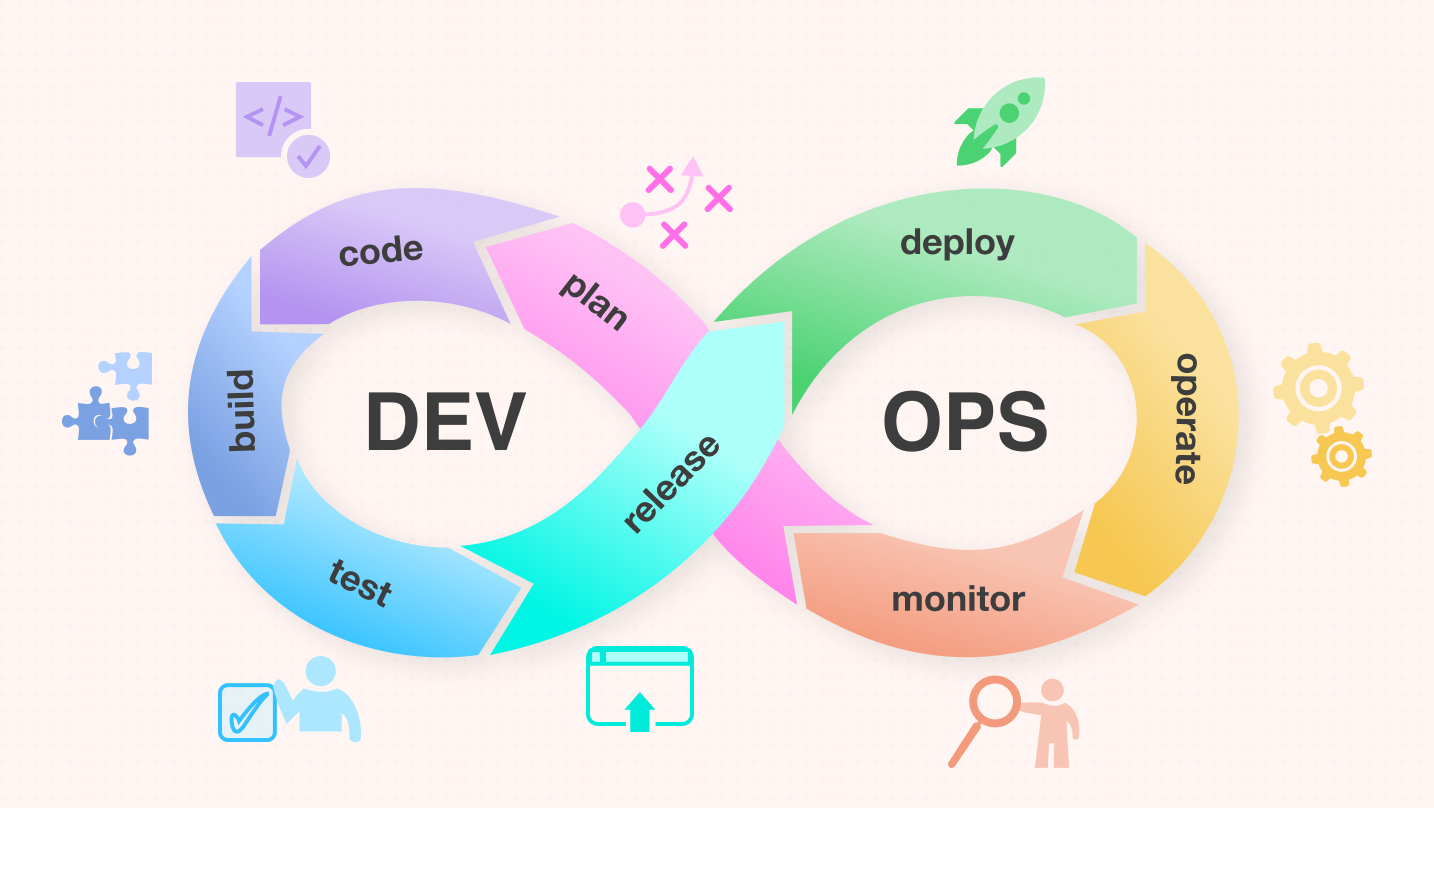
\includegraphics[width=0.9\textwidth]{src/assets/chapters/devopslifecycle.png}
  \caption{Application DevOps Lifecycle}
  \label{fig:application-devops-lifecycle}
\end{figure}

\subsection{Container management}
The use of containers has become one of the cornerstones of DevOps practice in recent times due to the efficiency and reliability that they add to the processes. But what are containers, and how do you manage them?

\textbf{What is a container ?}
\paragraph*{}
A container is a standard unit of software that packages up code and all its dependencies so the application runs quickly and reliably from one computing environment to another. They provide a lightweight virtualization which allows multiple containers to share the same machine but not the user space as an isolated one. 
In order to make the application portable.

\textbf{What is container management ?}
\paragraph*{}
Container management is the process for orchestrating and managing the containers whole lifecycle form creation, deployment to scaling and maintaining as well. As a result, tools such as Docker and  Podman are important which help with packing your applications into containers for deployment/management and keeping the manual workings of system administrators to an absolute minimum when it comes to applying updates/maintenance.

\subsection{CI/CD pipelines}
A CI/CD pipeline is a sequence of actions that need to be carried out to release a new version of software. The main aim of CI/CD pipelines is to enhance software delivery throughout the software development process through automation.


\section{Comparative Analysis}
To initiate our project, we require an extensive set of tools for managing version control, coordinating between containers, and deploy the application. Consequently, we conducted a comparative analysis of various tools available in the market.

\subsection{Version Control: Git vs SVN}
The most used tools for version control are Git and SVN. Here is a table
comparing both tools.


\begin{table}[h!]
  \centering
  \renewcommand{\arraystretch}{1.5} 
  \caption{Comparative study between Git and SVN}
  \label{tab: comparative_study_between_Git_and_SVN}
  \begin{tabularx}{\textwidth}{|>{\centering\arraybackslash}X|>{\centering\arraybackslash}X|}
      \hline
      \rowcolor{blue!20} 
      \textbf{Git} & \textbf{SVN} \\
      \hline
       Distributed version
control system & Centralized version
control system \\
      \hline
      Can work locally, offline & Must be connected to commit \\
      \hline
      Each user has a copy of the full repository & Each user only has a copy of the trunk  \\
      \hline
      Easy to fork, branch, and merge & Branching and merging is time-consuming  \\
      \hline
      Used by 90\% of developers & Used by 10\% of developers  \\
      \hline
  \end{tabularx}
\end{table}
Both choices are excellent in the final analysis.Nevertheless, we have decided to utilize Git since the company already operates a self-hosted GitLab instance that inherently supports Git.


\subsection{Container management: Docker vs Podman}
Even though Docker enjoys widespread popularity, Podman is also making its mark in the market, particularly on Red Hat systems.


\begin{table}[h!]
  \centering
  \renewcommand{\arraystretch}{1.5} 
  \caption{Comparative study between Docker and Podman}
  \label{tab: comparative_study_between_Docker_and_Podman}
  \begin{tabularx}{\textwidth}{|>{\centering\arraybackslash}X|>{\centering\arraybackslash}X|}
      \hline
      \rowcolor{blue!20} 
      \textbf{Docker} & \textbf{Podman} \\
      \hline
      Uses client-server architecture & Does not require a deamon to run, operates as a single command-line tool. \\
      \hline
      Docker daemon can run as non-root user & Podman uses a rootless mode by default, meaning that containers are run as regular users no with root privileges \\
      \hline
      Docker uses centralized image registry. Pull/push image to remote registry and load image from a local archive. & Podman uses a local image registry, which makes it easier to menage images locally.  \\
      \hline
      Docker uses a custom networking system. & podman relies on the standard Linus networking stack(more compatible with existing tools and systems).  \\
      \hline
  \end{tabularx}
\end{table}
The similarities between the two are apparent, and theoretically, the choice between Docker and Podman should be immaterial because both are interchangeable.


\subsection{Database: MongoDB vs PostgreSQL}
All old Aermax microservice are using a MongoDB database, but we did a comparative study between MongoDB and PostgreSQL to see if we should switch to PostgreSQL.


\begin{table}[h!]
  \centering
  \renewcommand{\arraystretch}{1.5} 
  \caption{Comparative study between MongDB and PostgreSQL}
  \label{tab: comparative_study_between_MongoDB_and_PostgreSQL}
  \begin{tabularx}{\textwidth}{|>{\centering\arraybackslash}X|>{\centering\arraybackslash}X|}
      \hline
      \rowcolor{blue!20} 
      \textbf{MongoDB} & \textbf{PostgreSQL} \\
      \hline
      mongoDB saves data as documents in the bson format & Rows and columns are used to store data in a tabular form. \\
      \hline
      Doesn't use schemas. Documents can be stored without defining their structure. & Uses schema \\
      \hline
      Uses Javascript to query a database. & Uses SQL to query a database.  \\
      \hline
      Supports horizontal scaling. & Supports vertical scaling.  \\
      \hline
  \end{tabularx}
\end{table}
Since the old architecture uses MongoDB, we will be sticking to that in the
new architecture as well for an easier migration.


\subsection{Database: GraphQL vs REST}
We have a decision to make regarding the data exchange in our application. We are considering the comparison between GraphQL and REST.


\begin{table}[h!]
  \centering
  \renewcommand{\arraystretch}{1.5} 
  \caption{Comparative study between REST and GraphQL }
  \label{tab: comparative_study_between_REST_and_GraphQL}
  \begin{tabularx}{\textwidth}{|>{\centering\arraybackslash}X|>{\centering\arraybackslash}X|}
      \hline
      \rowcolor{blue!20} 
      \textbf{REST} & \textbf{GraphQL} \\
      \hline
      Architectural style. & Query language. \\
      \hline
      Might require more than one endpoint. & Requires a signle endpoint. \\
      \hline
      Client can only ask for an entire resource. & Client can ask for a specific field of a resource.  \\
      \hline
      No typing.& Strongly typed.  \\
      \hline
      Cacheability. & No built-in caching.  \\
      \hline
       Updates might require new API versioning. & No API versioning.  \\
      \hline
        Non standard response(often XML or JSON) & Standard JSON response.  \\
      \hline
  \end{tabularx}
\end{table}
We decided to utilize REST due to limited time and implementing a new approach in a deliverable app won't be a good choice.


\subsection{Deployment: Kubernetes vs Docker Swarm}
Most deployments rely on Docker Compose, but it's not ideal for production, especially for systems that need to scale. After researching, we are considering using either Docker Swarm or Kubernetes.


\begin{table}[h!]
  \centering
  \renewcommand{\arraystretch}{1.5} 
  \caption{Comparative study between Kubernetes and Docker Swarm }
  \label{tab: comparative_study_between_kubernetes_and_Docker_swarm}
  \begin{tabularx}{\textwidth}{|>{\centering\arraybackslash}X|>{\centering\arraybackslash}X|}
      \hline
      \rowcolor{blue!20} 
      \textbf{Kubernetes} & \textbf{Docker Swarm} \\
      \hline
      Installation is complicated, but once setup, the cluster is very strong. & Installation is very simple, but cluster is not very strong. \\
      \hline
      GUI is the Kubernetes Dashboard & There is no GUI \\
      \hline
      Highly scalable and scales fast. & Highly scalable and scales 5x faster than Kubernetes.  \\
      \hline
      Kubernetes can do auto-scaling. & Docker Swarm can't do auto-scaling.  \\
      \hline
      Can deploy Rolling updates and does automatic Rollbacks. & Can deploy Rolling updates but not automatic Rollbacks.   \\
      \hline
      In-build tools for logging and monitoring. & 3rd party tools like ELK should be used for logging and monitoring.  \\
      \hline
      Can share storage volumes only with other containers in same Pod. & Can share storage volumes with any other containers.  \\
      \hline
  \end{tabularx}
\end{table}
Hence, we plan to implement our application stack on Kubernetes due to its significant potential, especially when compared to the outdated Docker Swarm.

\newpage
\subsection{Deployment management: Kubectl vs Helm}
Given that we are utilizing Kubernetes, we have the choice to deploy our microservices using either Kubectl or Helm.


\begin{table}[h!]
  \centering
  \renewcommand{\arraystretch}{1.5} 
  \caption{Comparative study between Helm and Kubectl}
  \label{tab:comparative_study_between_helm_and_kubectl}
  \begin{tabularx}{\textwidth}{|>{\centering\arraybackslash}X|>{\centering\arraybackslash}X|}
      \hline
      \rowcolor{blue!20} 
      \textbf{Helm} & \textbf{Kubectl} \\
      \hline
      Helm serves as the package manager for Kubernetes, in essence. & The official Kubernetes command-line tool is Kubectl, which permits the execution of commands against Kubernetes clusters. \\
      \hline
      Simplifies deployment of complex applications. & Requires detailed configuration for each resource.  \\
      \hline
      Uses templates for Kubernetes manifests, supports variables and conditionals. & Directly applies Kubernetes YAML files without templating.  \\
      \hline
      Manages application versions and rollbacks easily. & Version control and rollbacks must be handled manually.  \\
      \hline
      Uses Helm charts to package applications, making reuse and sharing easy. & Does not have a native concept of charts; relies on YAML files.   \\
      \hline
  \end{tabularx}
\end{table}
After carefully analyzing our use case, we decided to develop a consistent Helm package for deploying our microservices.
Additionally, we found it important to establish standard configurations that we can easily apply using Kubectl, including Ingress rules, for convenience and due to time constraints.

\subsection{Conclusion}
In this section, we explored the key principles related to our project, including web scraping, automation, and DevOps. Next, we delved into various available tools and deliberated on our selections.


\section{Main Setup}
\subsection{Introduction}
In this section, we will address the much-anticipated realization. This phase involves putting into action all the groundwork laid in the preceding sections. DevOps will be a major focus in this part, as our main goal has been to deploy the reward system to a scalable architecture using contemporary DevOps practices. We will commence with the hardware and software configuration of the new architecture, followed by an exploration of how to oversee the entire application stack.

\subsection{Hardware setup}
Given that we have decided to move forward with the self-managed Kubernetes deployment, we will need to establish our own cluster nodes or virtual machines. These nodes can be categorized into core nodes, which are established once, and scalable nodes, which can be generated as needed for scaling purposes.
\subsubsection{Cloud provider}
We plan to utilize the Hetzner Cloud provider to allocate the necessary hardware resources for the deployment.

\begin{figure}[H]
  \centering
  
\includegraphics[width=0.4\textwidth]{src/assets/chapters/hetzner.png}
  \caption{Logo of Hetzner}
  \label{fig:cloud-provider}
\end{figure}



Hetzner Cloud, utilizing its Hetzner CloudPanel service, provides a platform that is easy for users to create and oversee virtual machines, configure firewall rules, set up private networks, and manage other essential infrastructure components.

\begin{figure}[H]
  \centering
  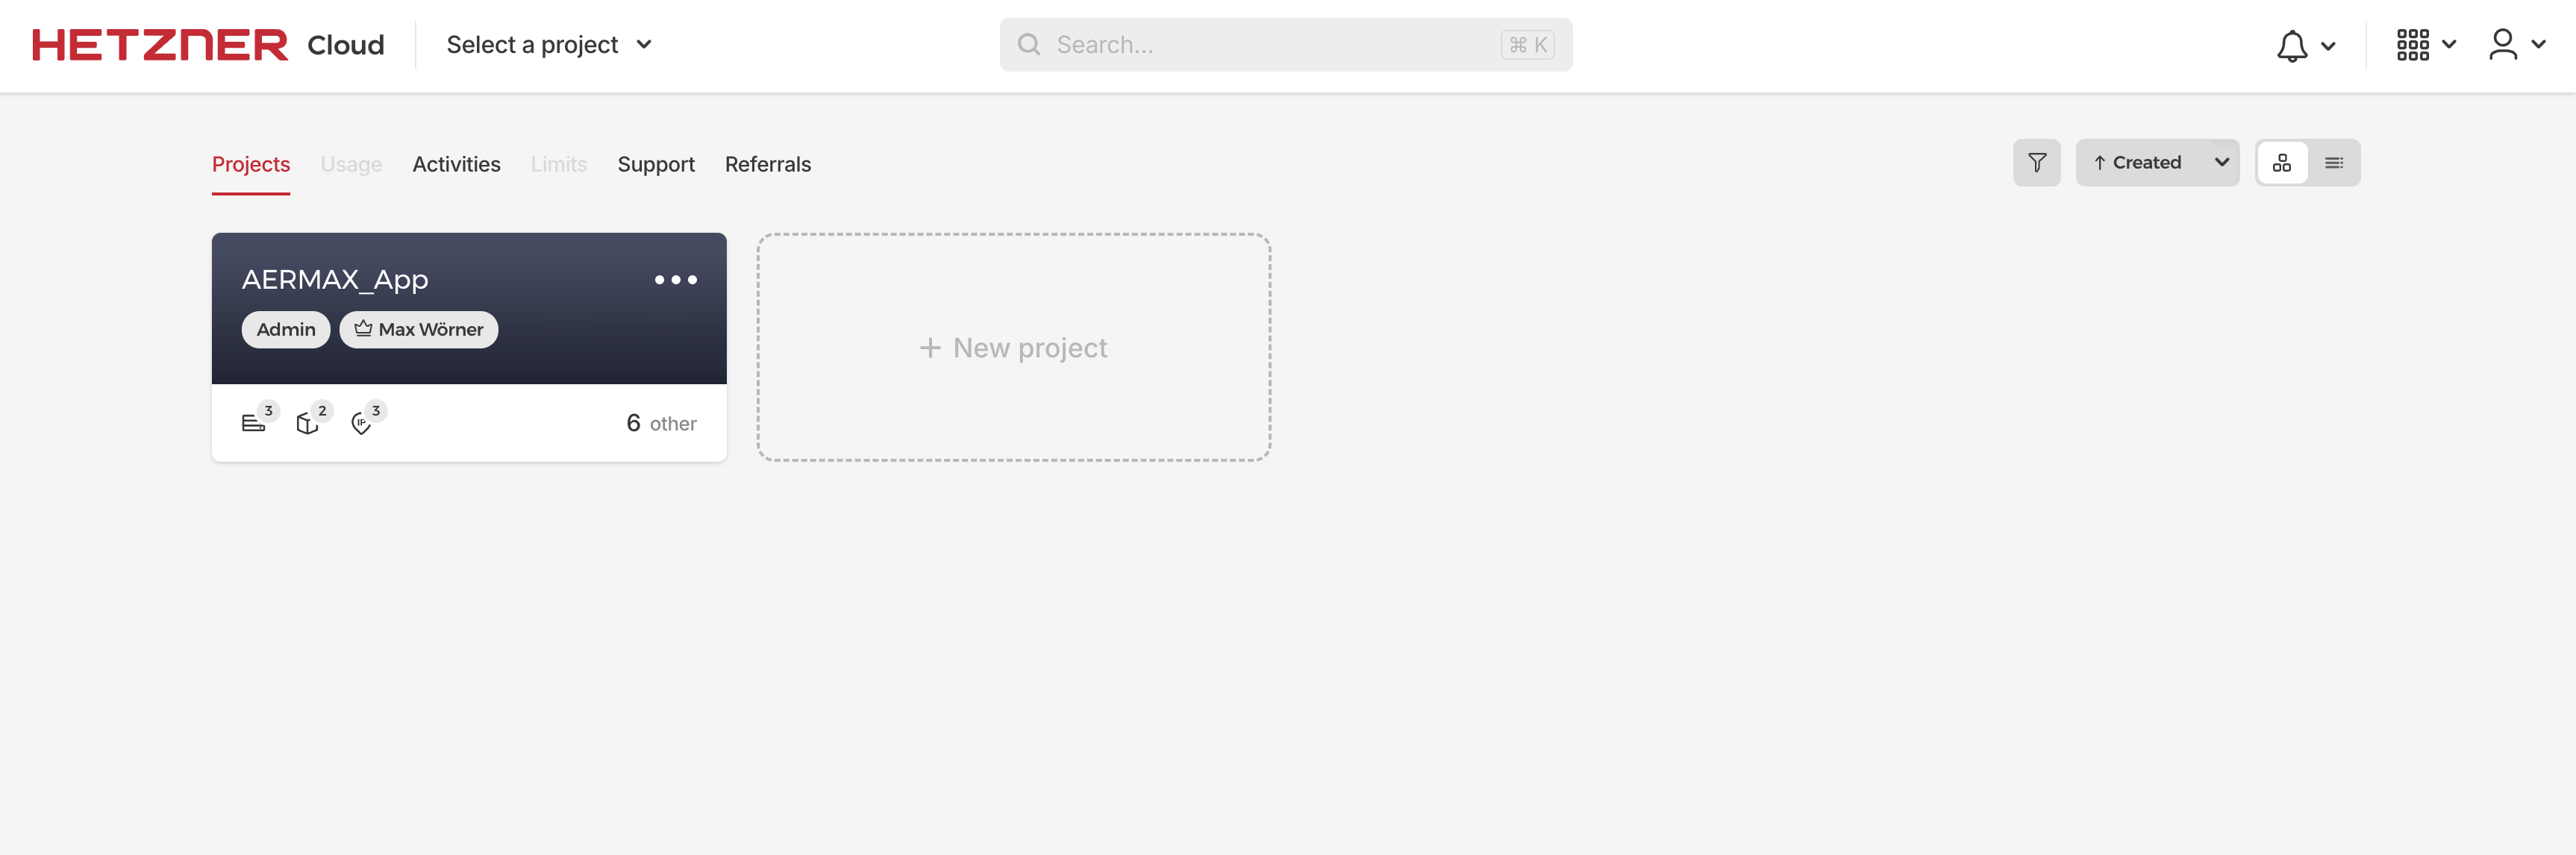
\includegraphics[width=1\textwidth]{src/assets/chapters/cloudproject.png}
  \caption{Hetzner Cloud Project Overview}
  \label{fig:cloud-project-overview}
\end{figure}

The Hetzner Cloudpanel dashboard provides the following deployment options:

\begin{itemize}
  \item \textbf{Servers:} This section allows users to create and manage virtual machines.
  \item \textbf{Volumes:} This section allows users to create and manage volumes(A Volume is a highly-available, scalable, and SSD-based block storage for Servers.).
  \item \textbf{Networks:} Networks is a private networks feature. These Networks are optional and they coexist with the public network that every Server has by default.

  \item \textbf{Firewalls:} This section allows users to create and manage firewall rules(Firewalls can limit the network access to or from your resources).
\end{itemize}




\begin{figure}[H]
  \centering
  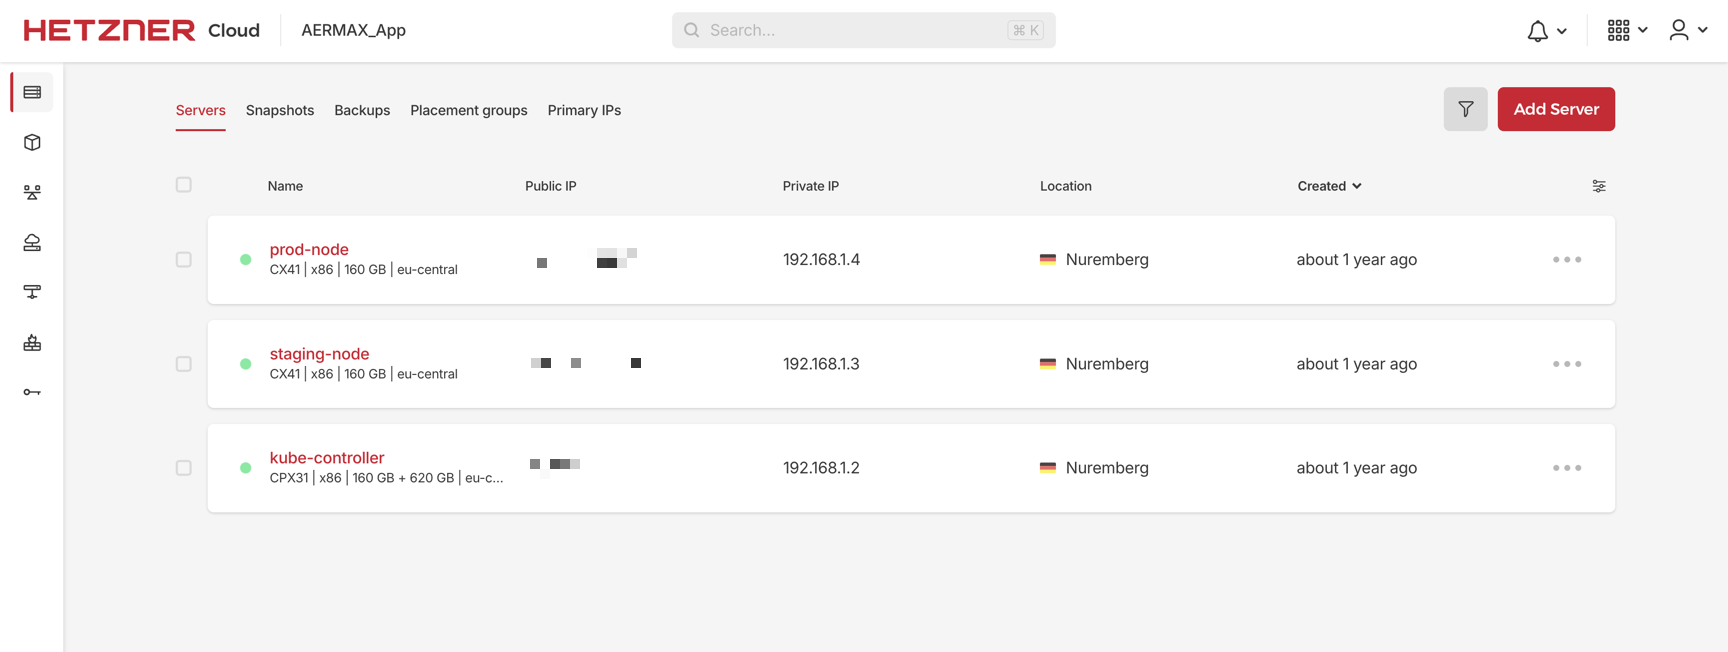
\includegraphics[width=1\textwidth]{src/assets/chapters/servers.png}
  \caption{Hetzner Cloud Servers Overview}
  \label{fig:cloud-project-servers-overview}
\end{figure}

\begin{figure}[H]
  \centering
  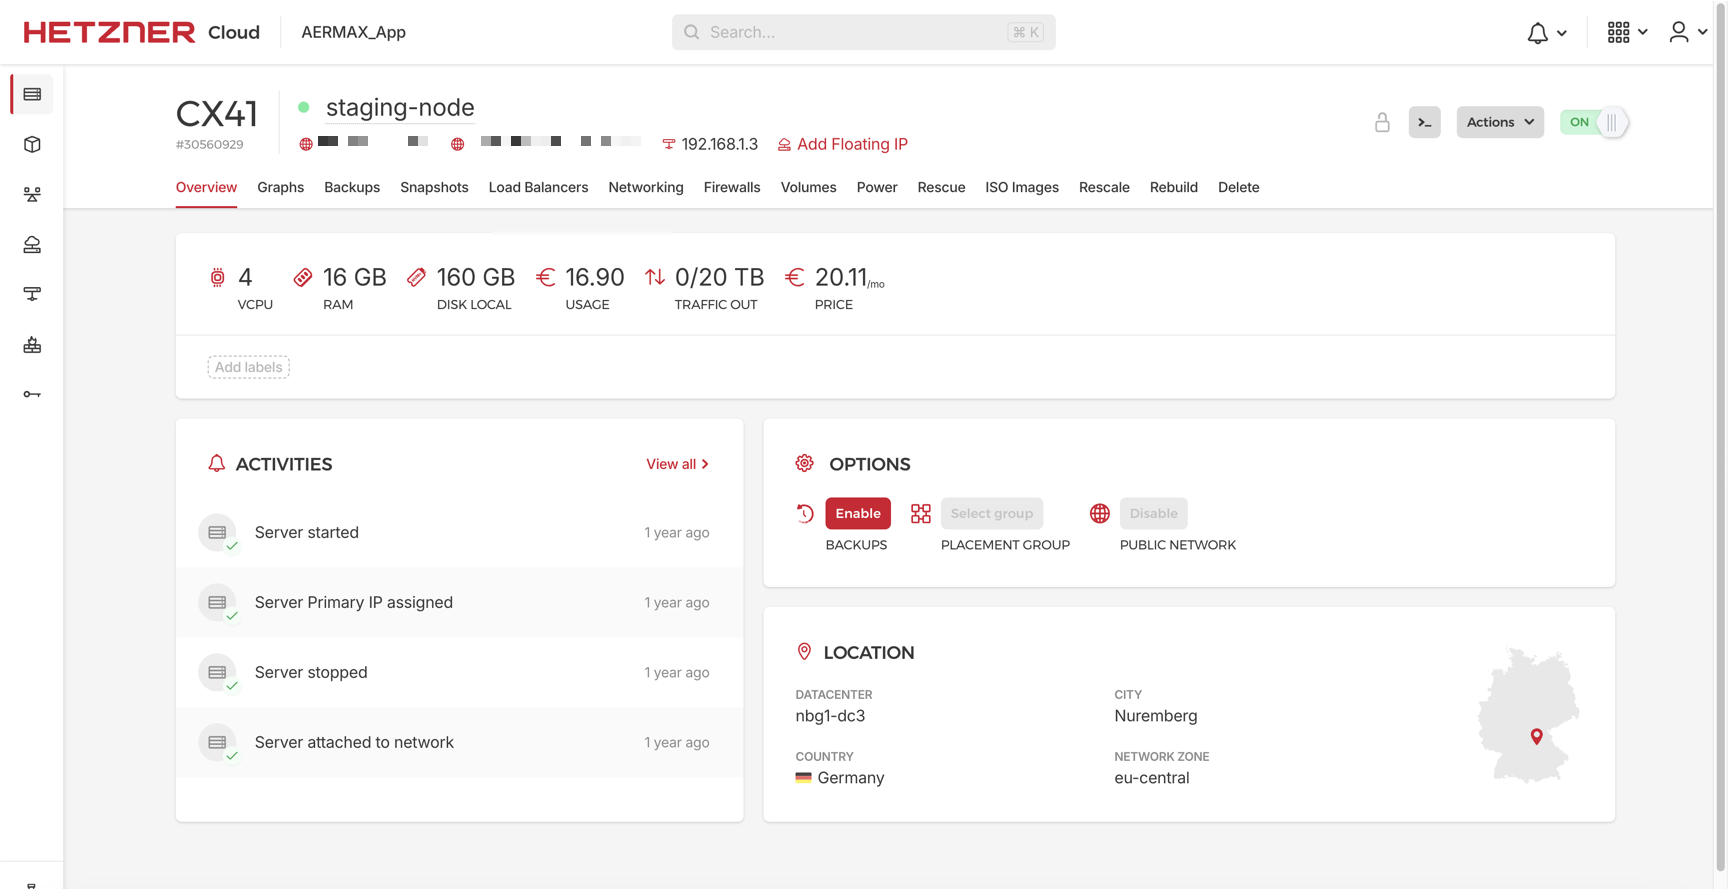
\includegraphics[width=1\textwidth]{src/assets/chapters/serversoverview.png}
  \caption{Hetzner Cloud Server Details}
  \label{fig:cloud-project-server-details}
\end{figure}

\begin{figure}[H]
  \centering
  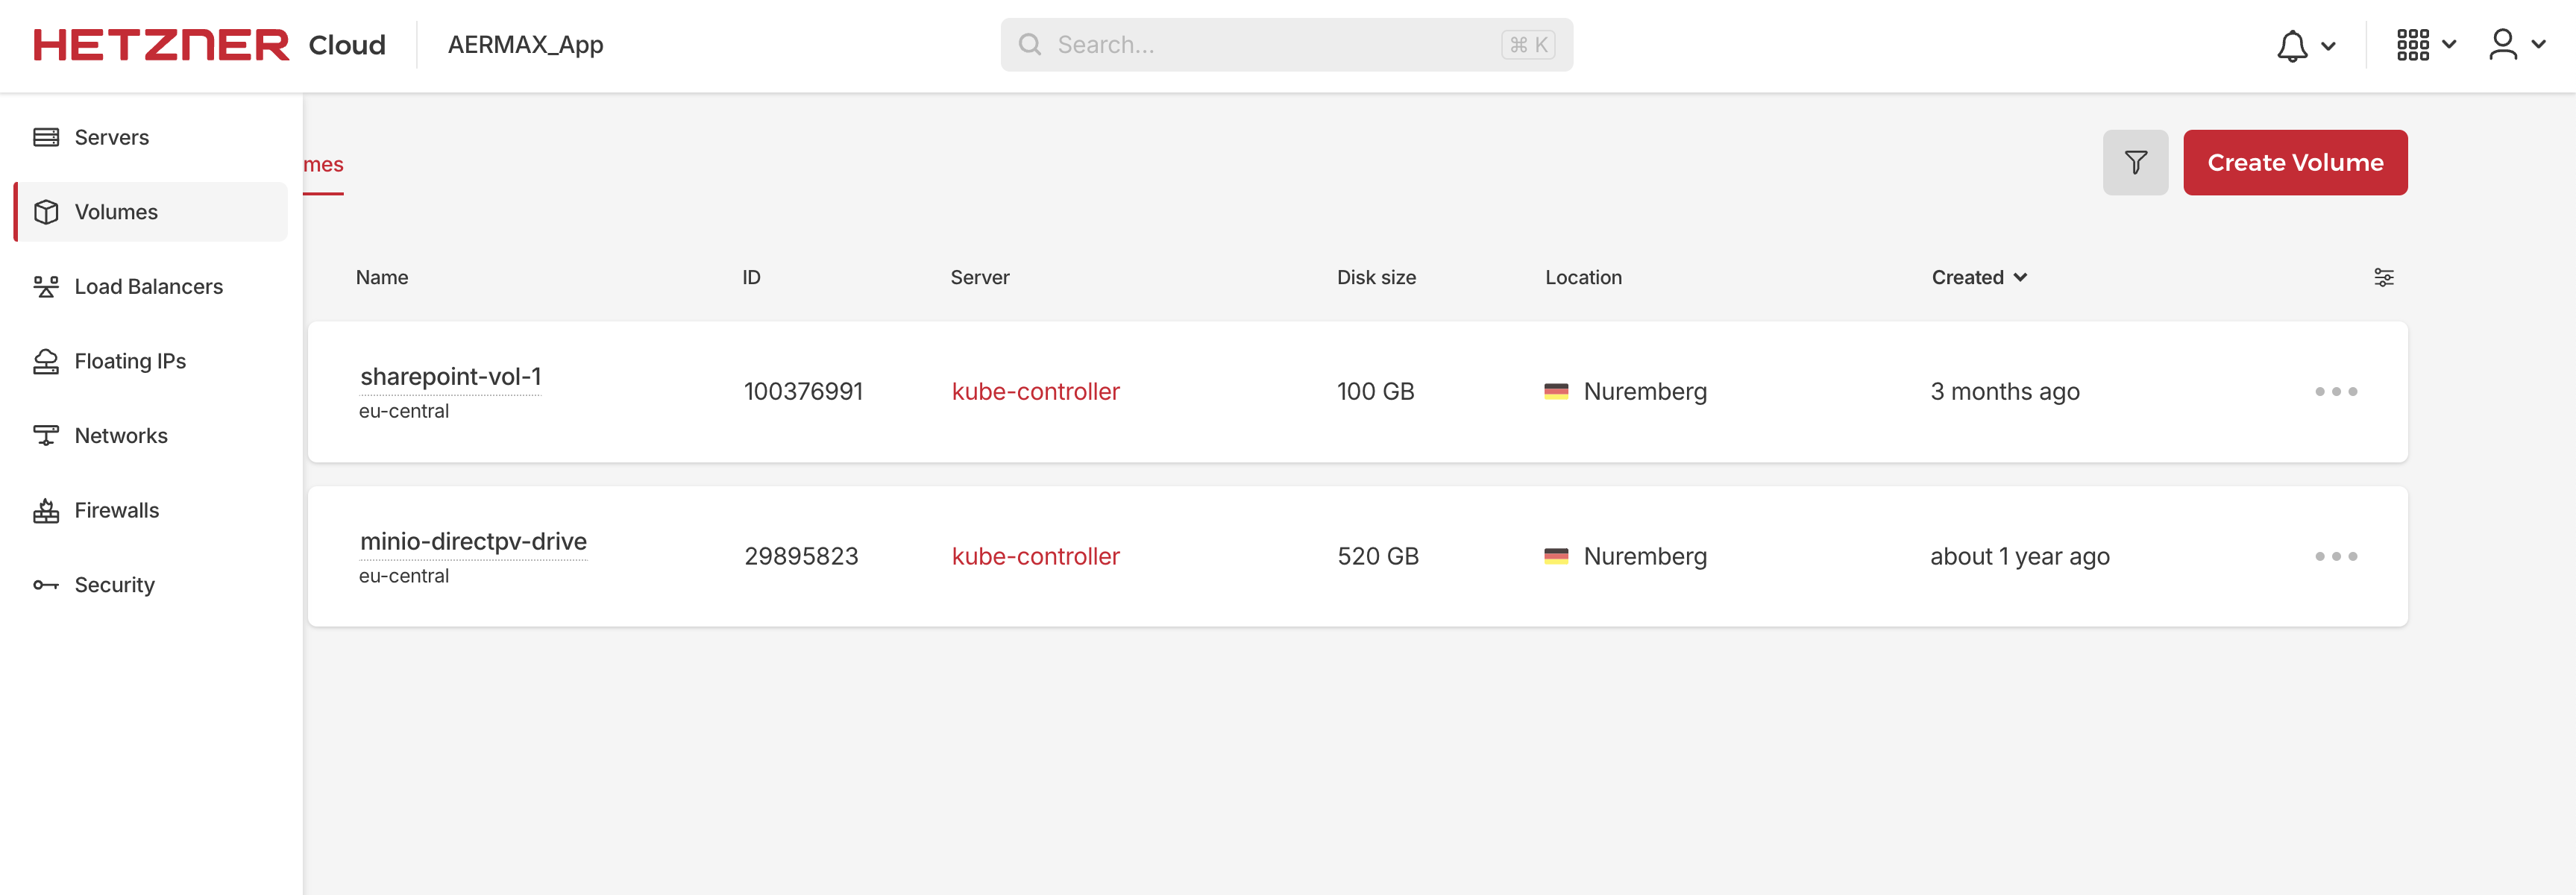
\includegraphics[width=1\textwidth]{src/assets/chapters/volumes.png}
  \caption{Hetzner Cloud Volumes}
  \label{fig:cloud-project-volumes}
\end{figure}

\begin{figure}[H]
  \centering
  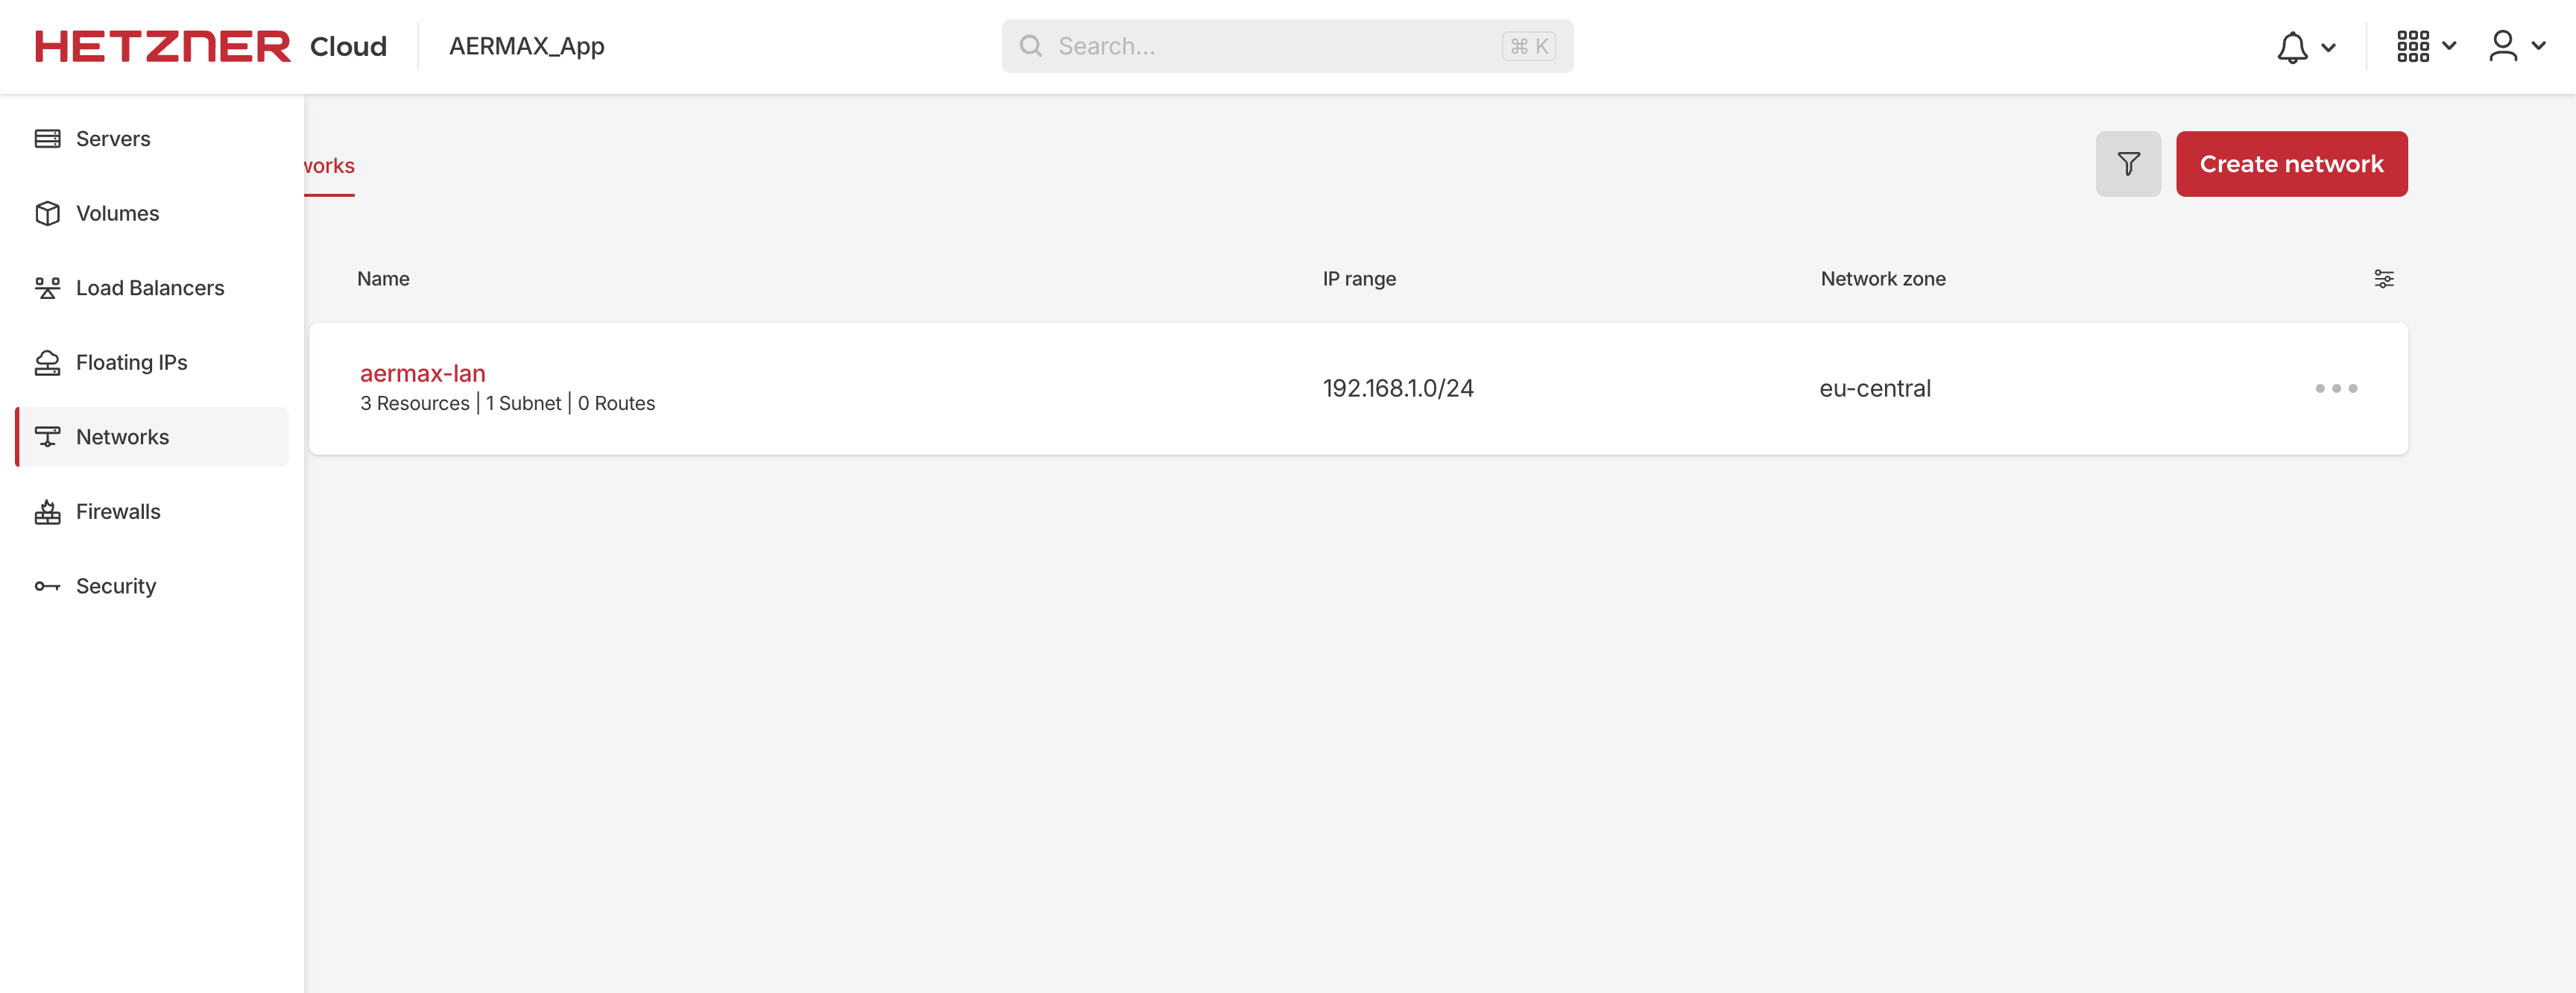
\includegraphics[width=1\textwidth]{src/assets/chapters/networks.png}
  \caption{Hetzner Cloud Networks}
  \label{fig:cloud-project-networks}
\end{figure}


\begin{figure}[H]
  \centering
  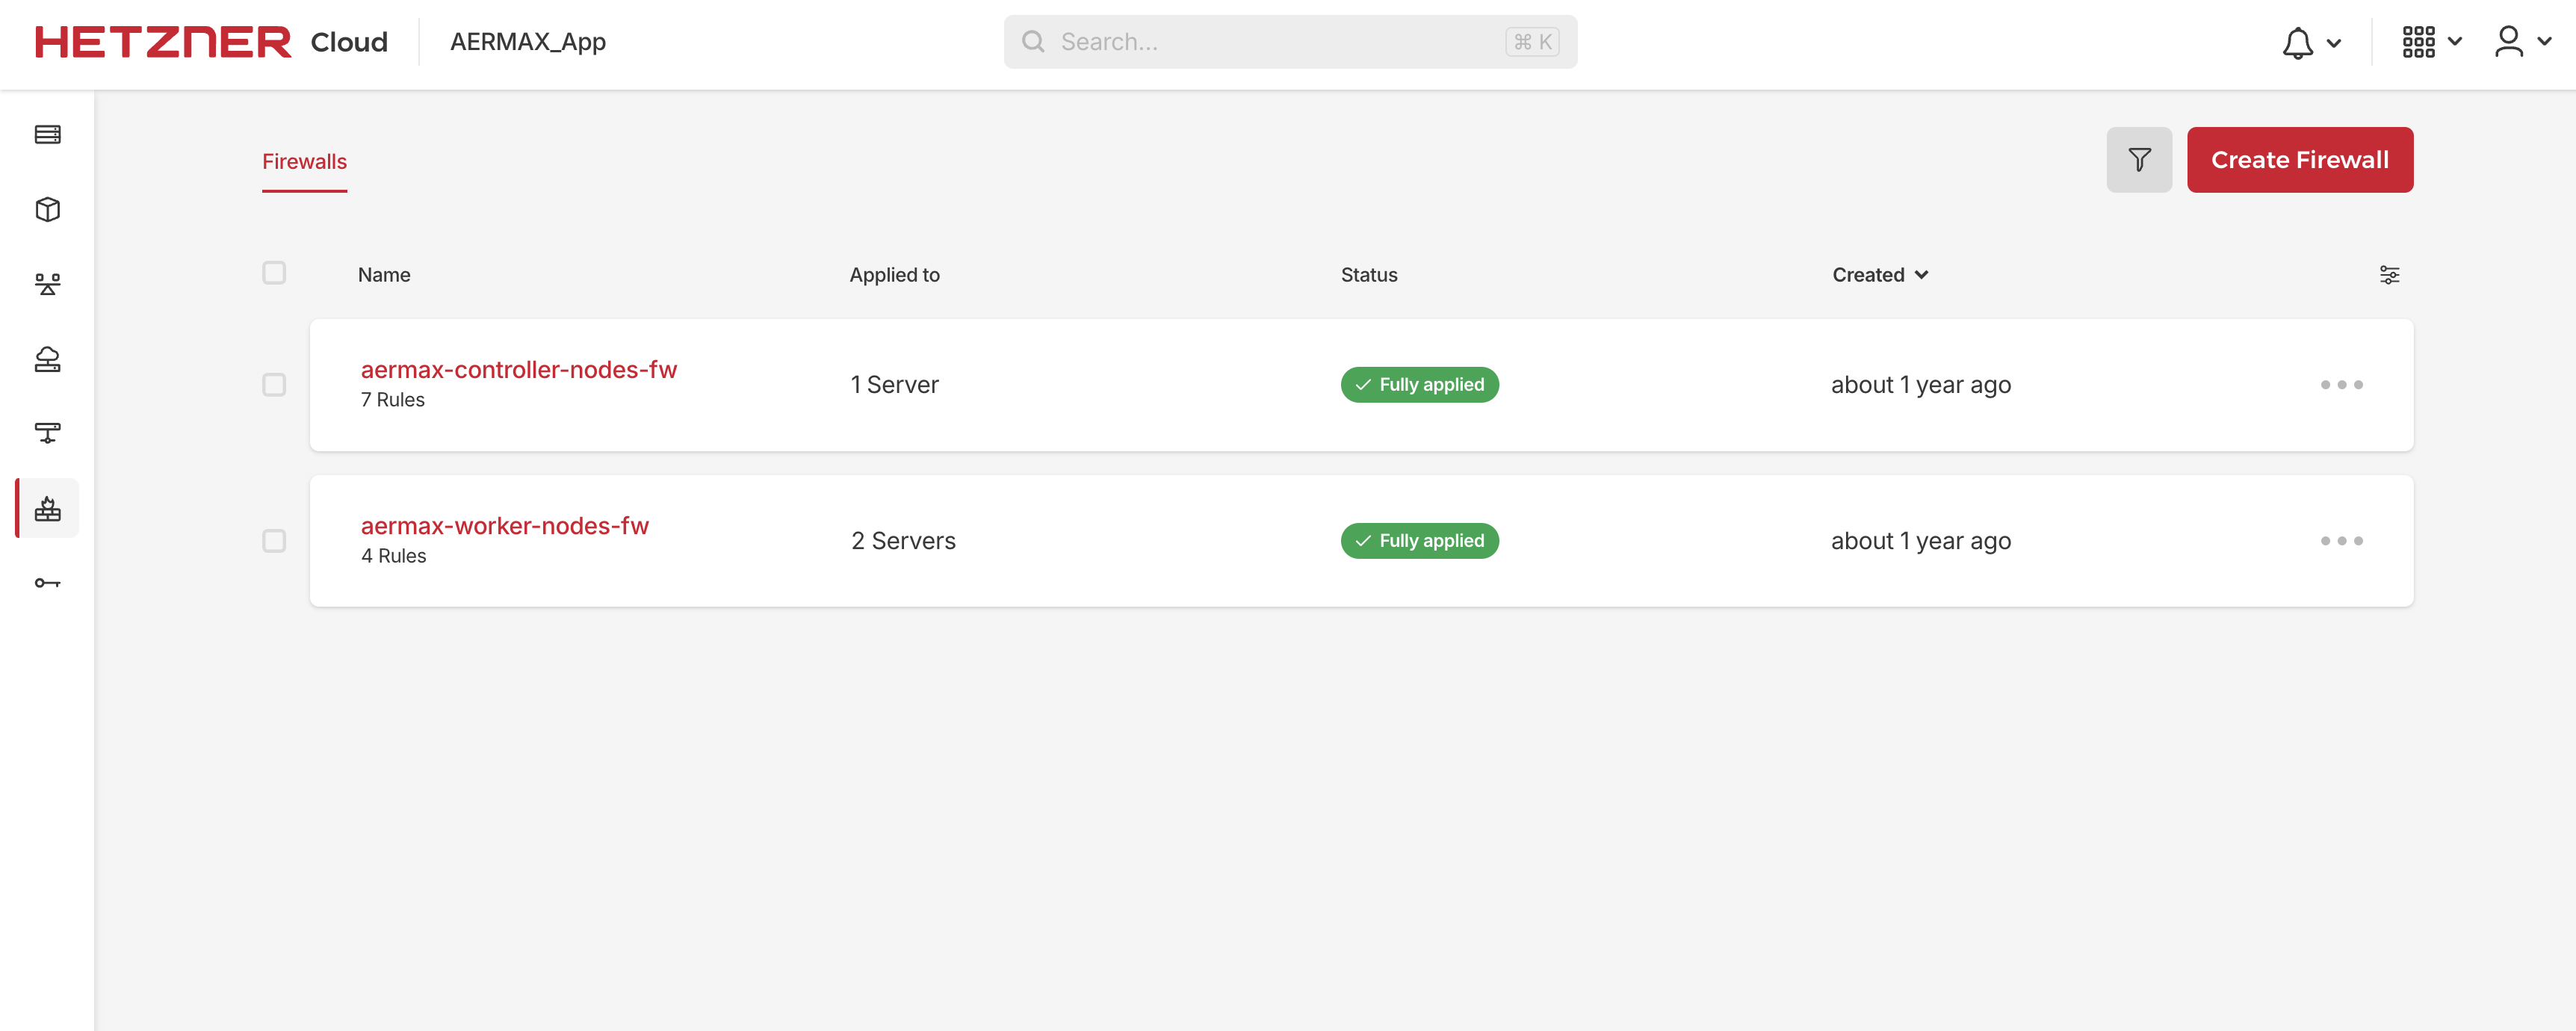
\includegraphics[width=1\textwidth]{src/assets/chapters/firewall.png}
  \caption{Hetzner Cloud Firewalls}
  \label{fig:cloud-project-fw}
\end{figure}


\subsubsection{Kubernetes Cluster}
Using the cloudpanel dashboard, now is the moment to establish our cluster. The following tables display the virtual machines required to begin.

\begin{figure}[H]
  \centering
  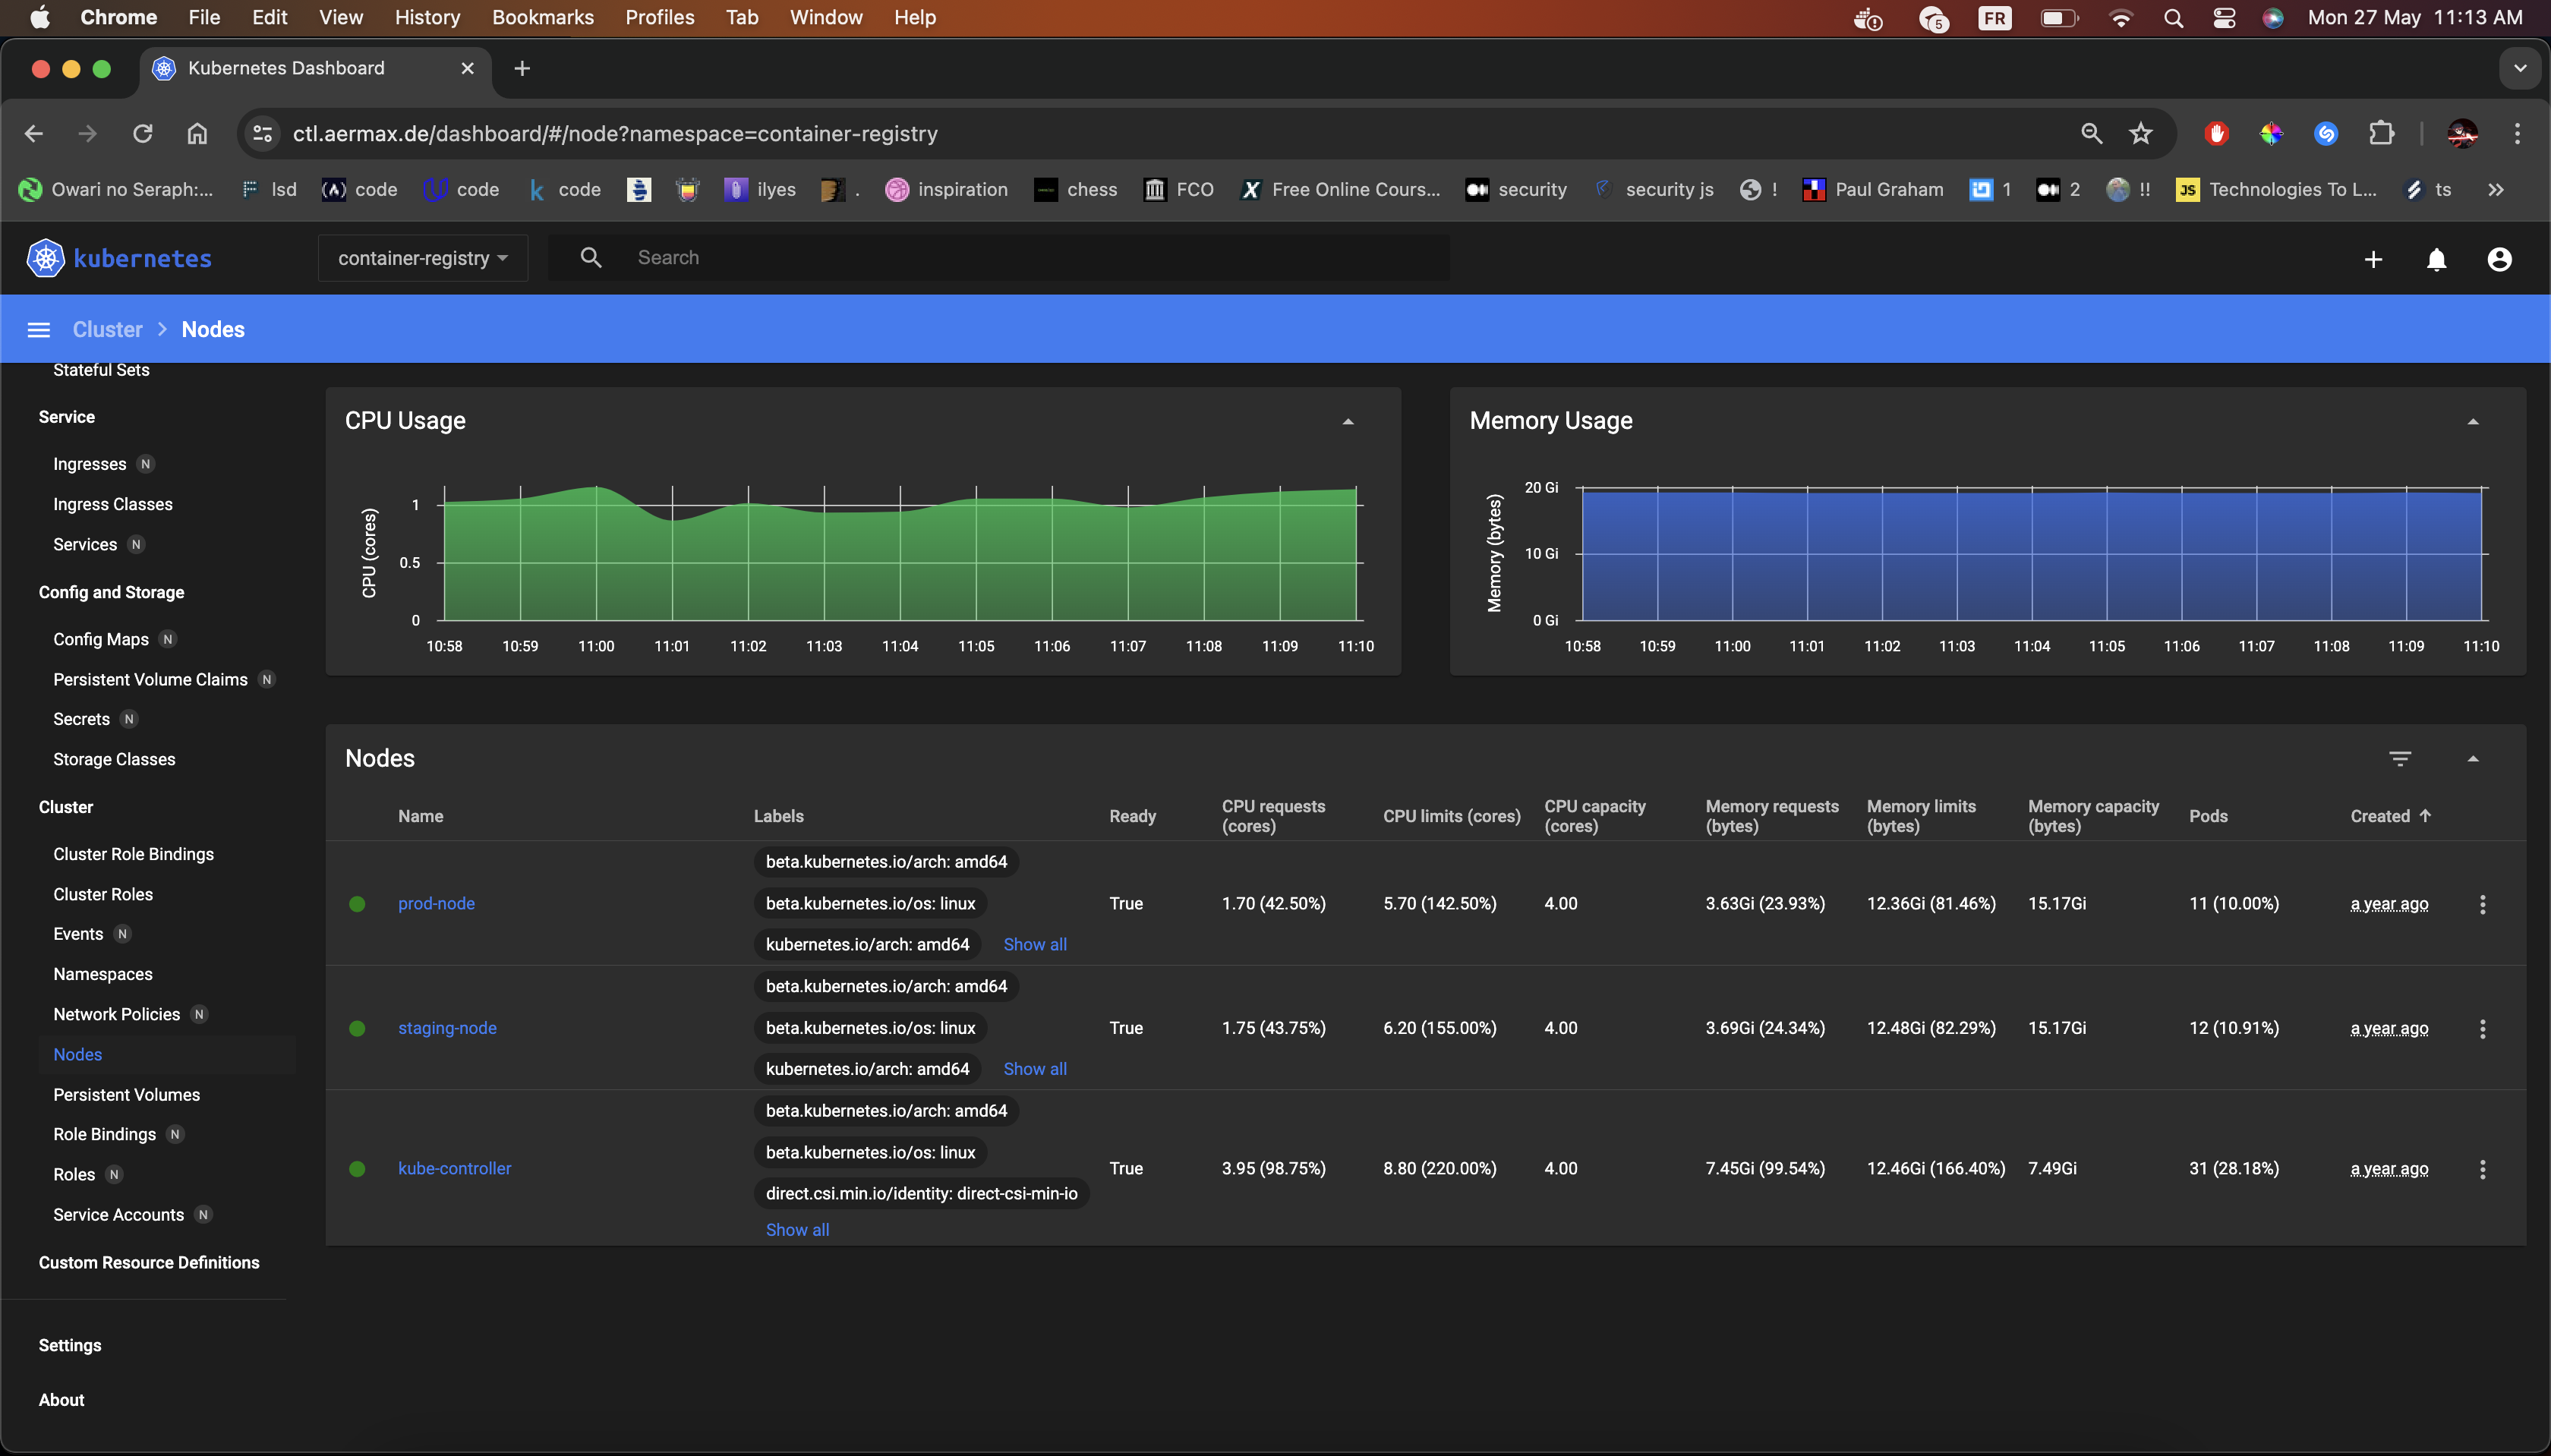
\includegraphics[width=1\textwidth]{src/assets/chapters/kubernodes.png}
  \caption{Kubernetes Dashboard Core Nodes}
  \label{fig:kubernodes}
\end{figure}

\begin{figure}[H]
  \centering
  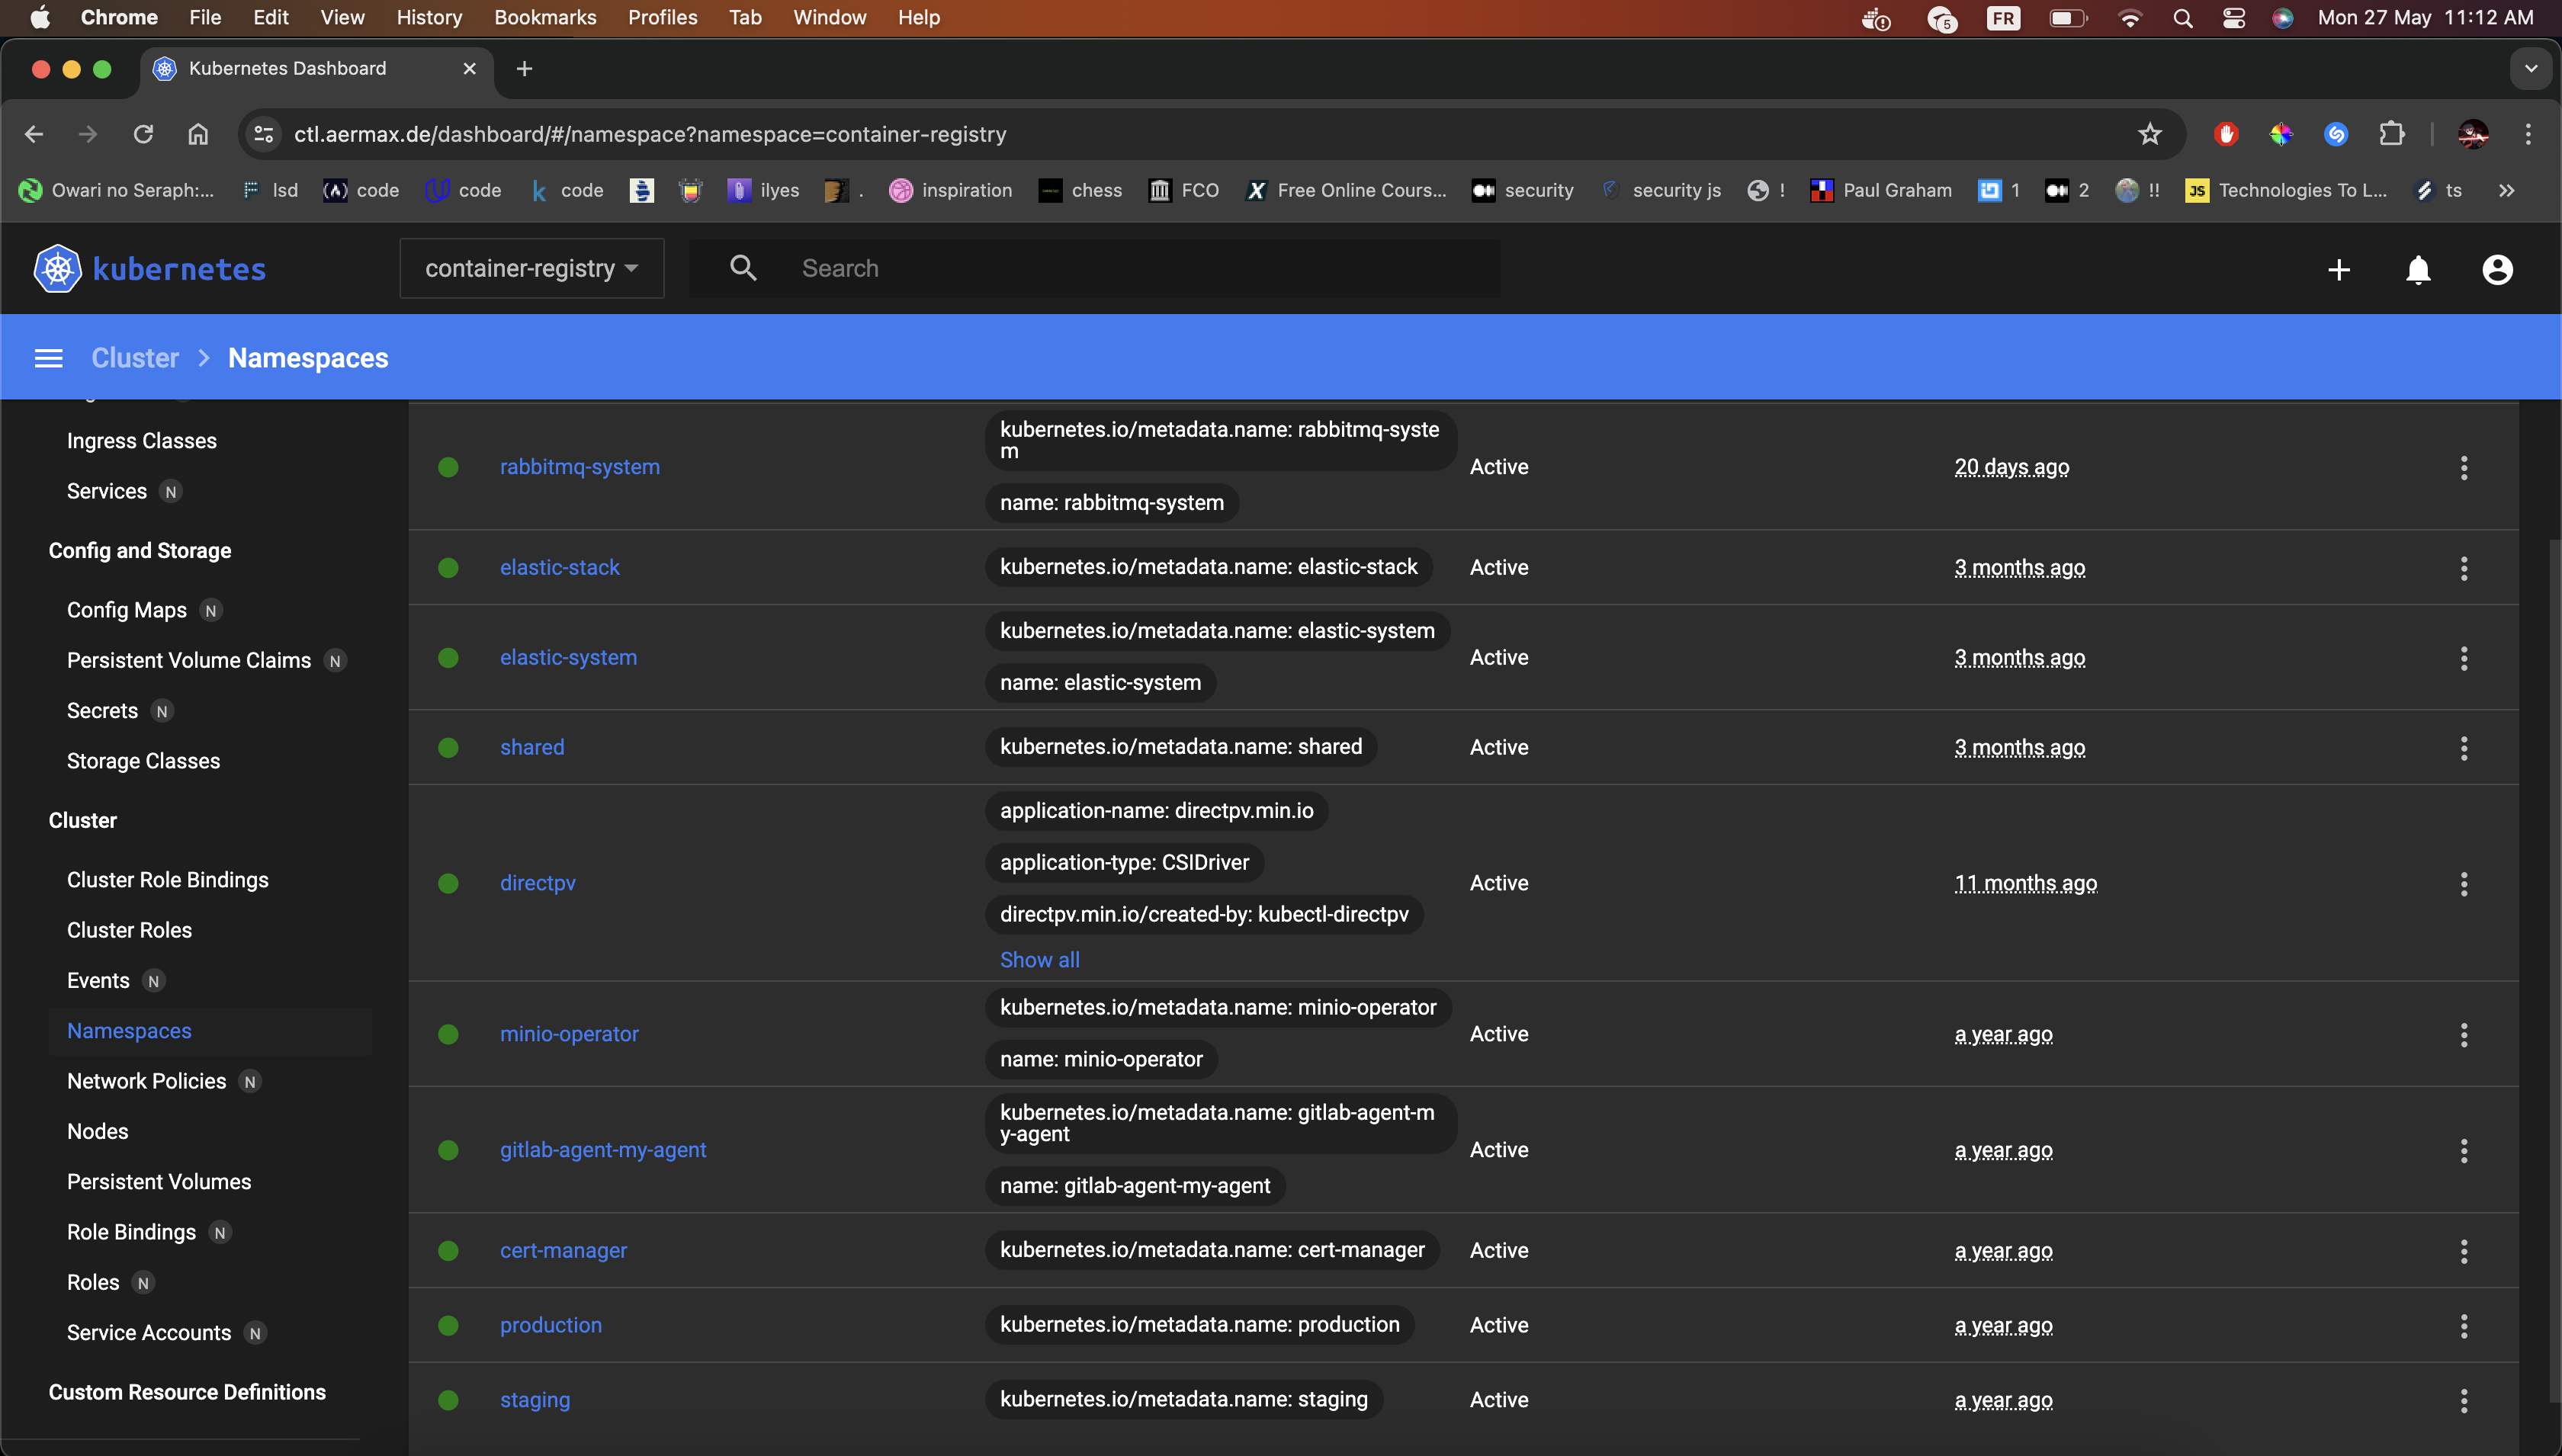
\includegraphics[width=1\textwidth]{src/assets/chapters/kubernamespaces.png}
  \caption{Kubernetes Dashboard Namespaces}
  \label{fig:kubernamespaces}
\end{figure}

\begin{table}[h!]
  \centering
  \renewcommand{\arraystretch}{1.5} 
  \caption{ Core cluster nodes}
  \label{tab: core_cluster_nodes}
  \begin{tabularx}{\textwidth}{|>{\centering\arraybackslash}X|>{\centering\arraybackslash}X|>{\centering\arraybackslash}X|}
      \hline
      \rowcolor{blue!20} 
      \textbf{Name} & \textbf{Services Swarm} & \textbf{Size} \\
      \hline
      kube-controller & The main Kubernetes cluster controller  & XL \\
      \hline
      prod-node & Elastic-stack, Ngnix Ingress, Keyclock, RabbitMq, all other Aermax services  & L \\
      \hline
      staging-node & Elastic-stack, Ngnix Ingress, Keyclock, RabbitMq, all other Aermax services  & L \\
      \hline
  \end{tabularx}
\end{table}


\subsection{Software setup}
After our hardware resources are set up, we have raw Linux virtual machines with no configuration. To move forward, we must create and handle our own Kubernetes instance using MicroK8s. Before doing that, we also need to establish some basic configurations.

\subsubsection{Manual configuration}
For a single virtual machine, we have to do the following setup:

\begin{itemize}
  \item Set up a user with elevated privileges
  \item Download and set up the essential packages for our use
  \item Modify the hosts file to enable the virtual machine to identify other virtual machines by their hostnames
  \item Deploy MicroK8s to establish a single-node cluster on the virtual machine
  \item Connect the virtual machine to the master node to form a multi-node cluster.
\end{itemize}

\subsection{Deployment process}
We will now describe the strategy we have implemented for continuously integrating, deploying, and delivering our application, in line with the DevOps best practices. At present, the deployment is backed by two distinct environments: the staging environment for validating the proper functioning of our application, and the production environment.

\subsubsection{Adopted strategy}
Given that we have multiple microservices, it's not practical to interact with our Kubernetes cluster from each one every time we make a change. As a result, we follow these steps to deploy our application:

\begin{itemize}
  \item When we have updates in any of our microservices, we generate a new Docker image and upload it to a dedicated container registry.
  \item After the build process finishes, we trigger a multi-project pipeline leading to a central repository named "aermax-controller."
  \item This central repository then communicates with our Kubernetes cluster to deploy the application to the correct environment, using a custom Helm package that we developed. Additional information is available in the subsequent sections.

\end{itemize}

\paragraph{}
This is further explained in detail in the following sub sections.

\subsubsection{Linking the cluster to GitLab}
We plan to connect our Kubernetes cluster with GitLab using the GitLab Kubernetes Agent, also known as KAS.


\begin{figure}[H]
  \centering
  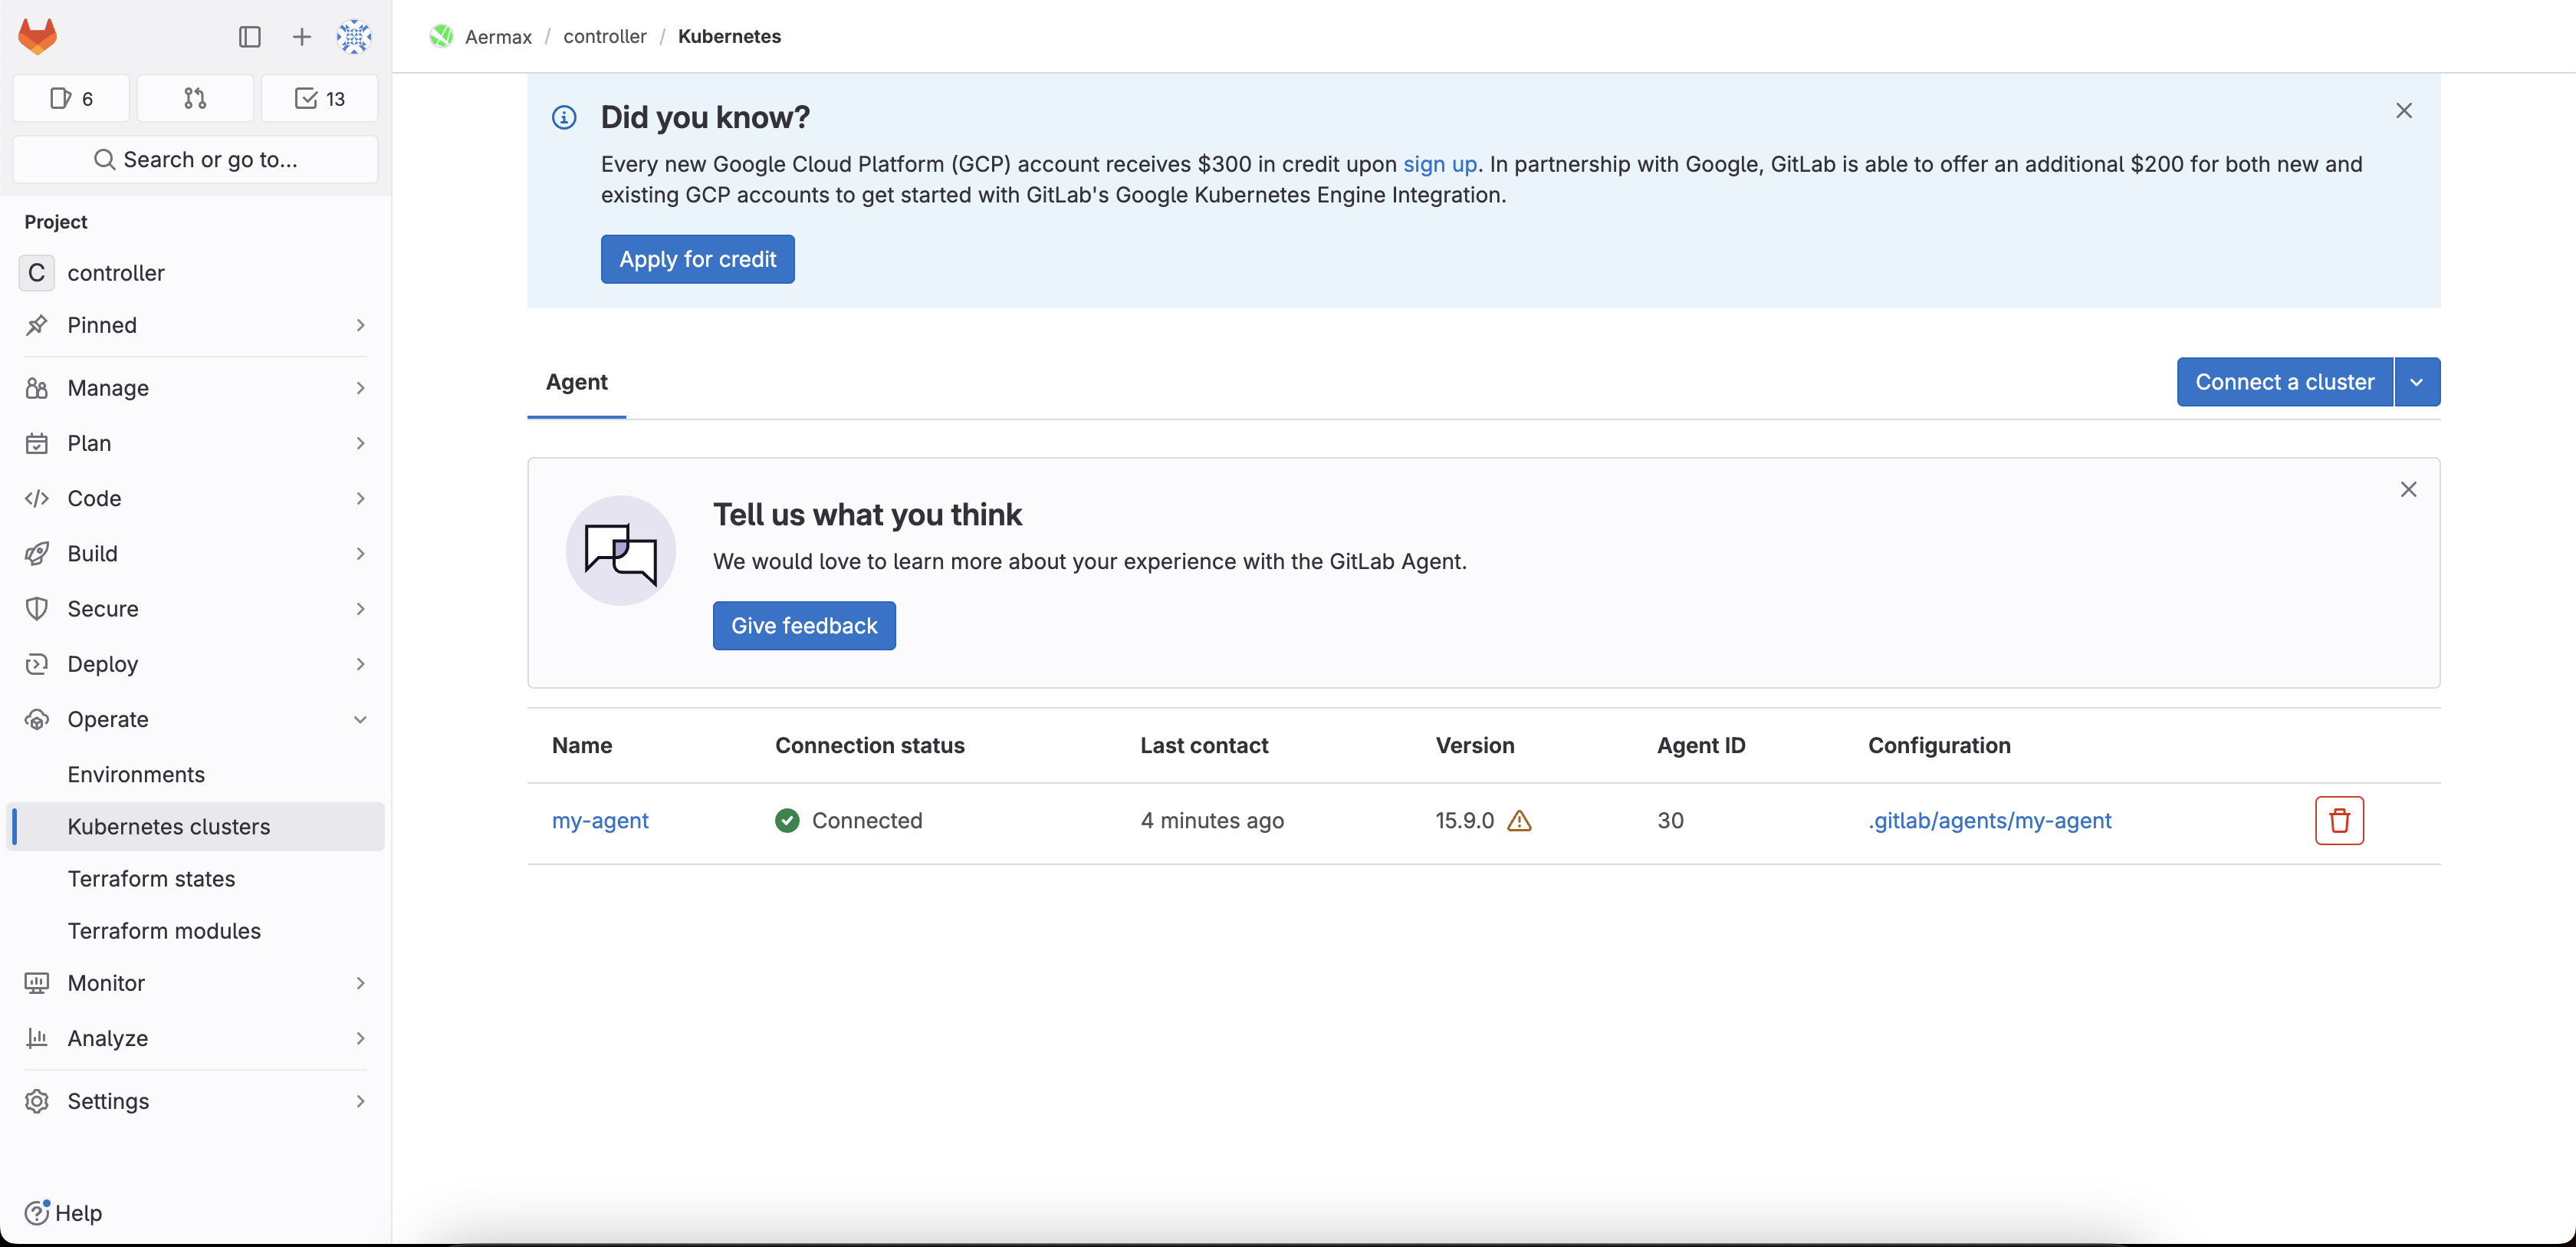
\includegraphics[width=1\textwidth]{src/assets/chapters/linkingrepowithkuber.png}
  \caption{GitLab Kubernetes Agent}
  \label{fig:gitlab-kuber}
\end{figure}


\subsubsection{Continuous Integration}
Every time a developer makes changes in the main branch of a microservice, automatic tests are run. Assuming that everything passed, a Docker image with the changes will be uploaded to the container registry, and our deployment process will start. Finally, the new code will be put into place, marking the.


\begin{figure}[H]
  \centering
  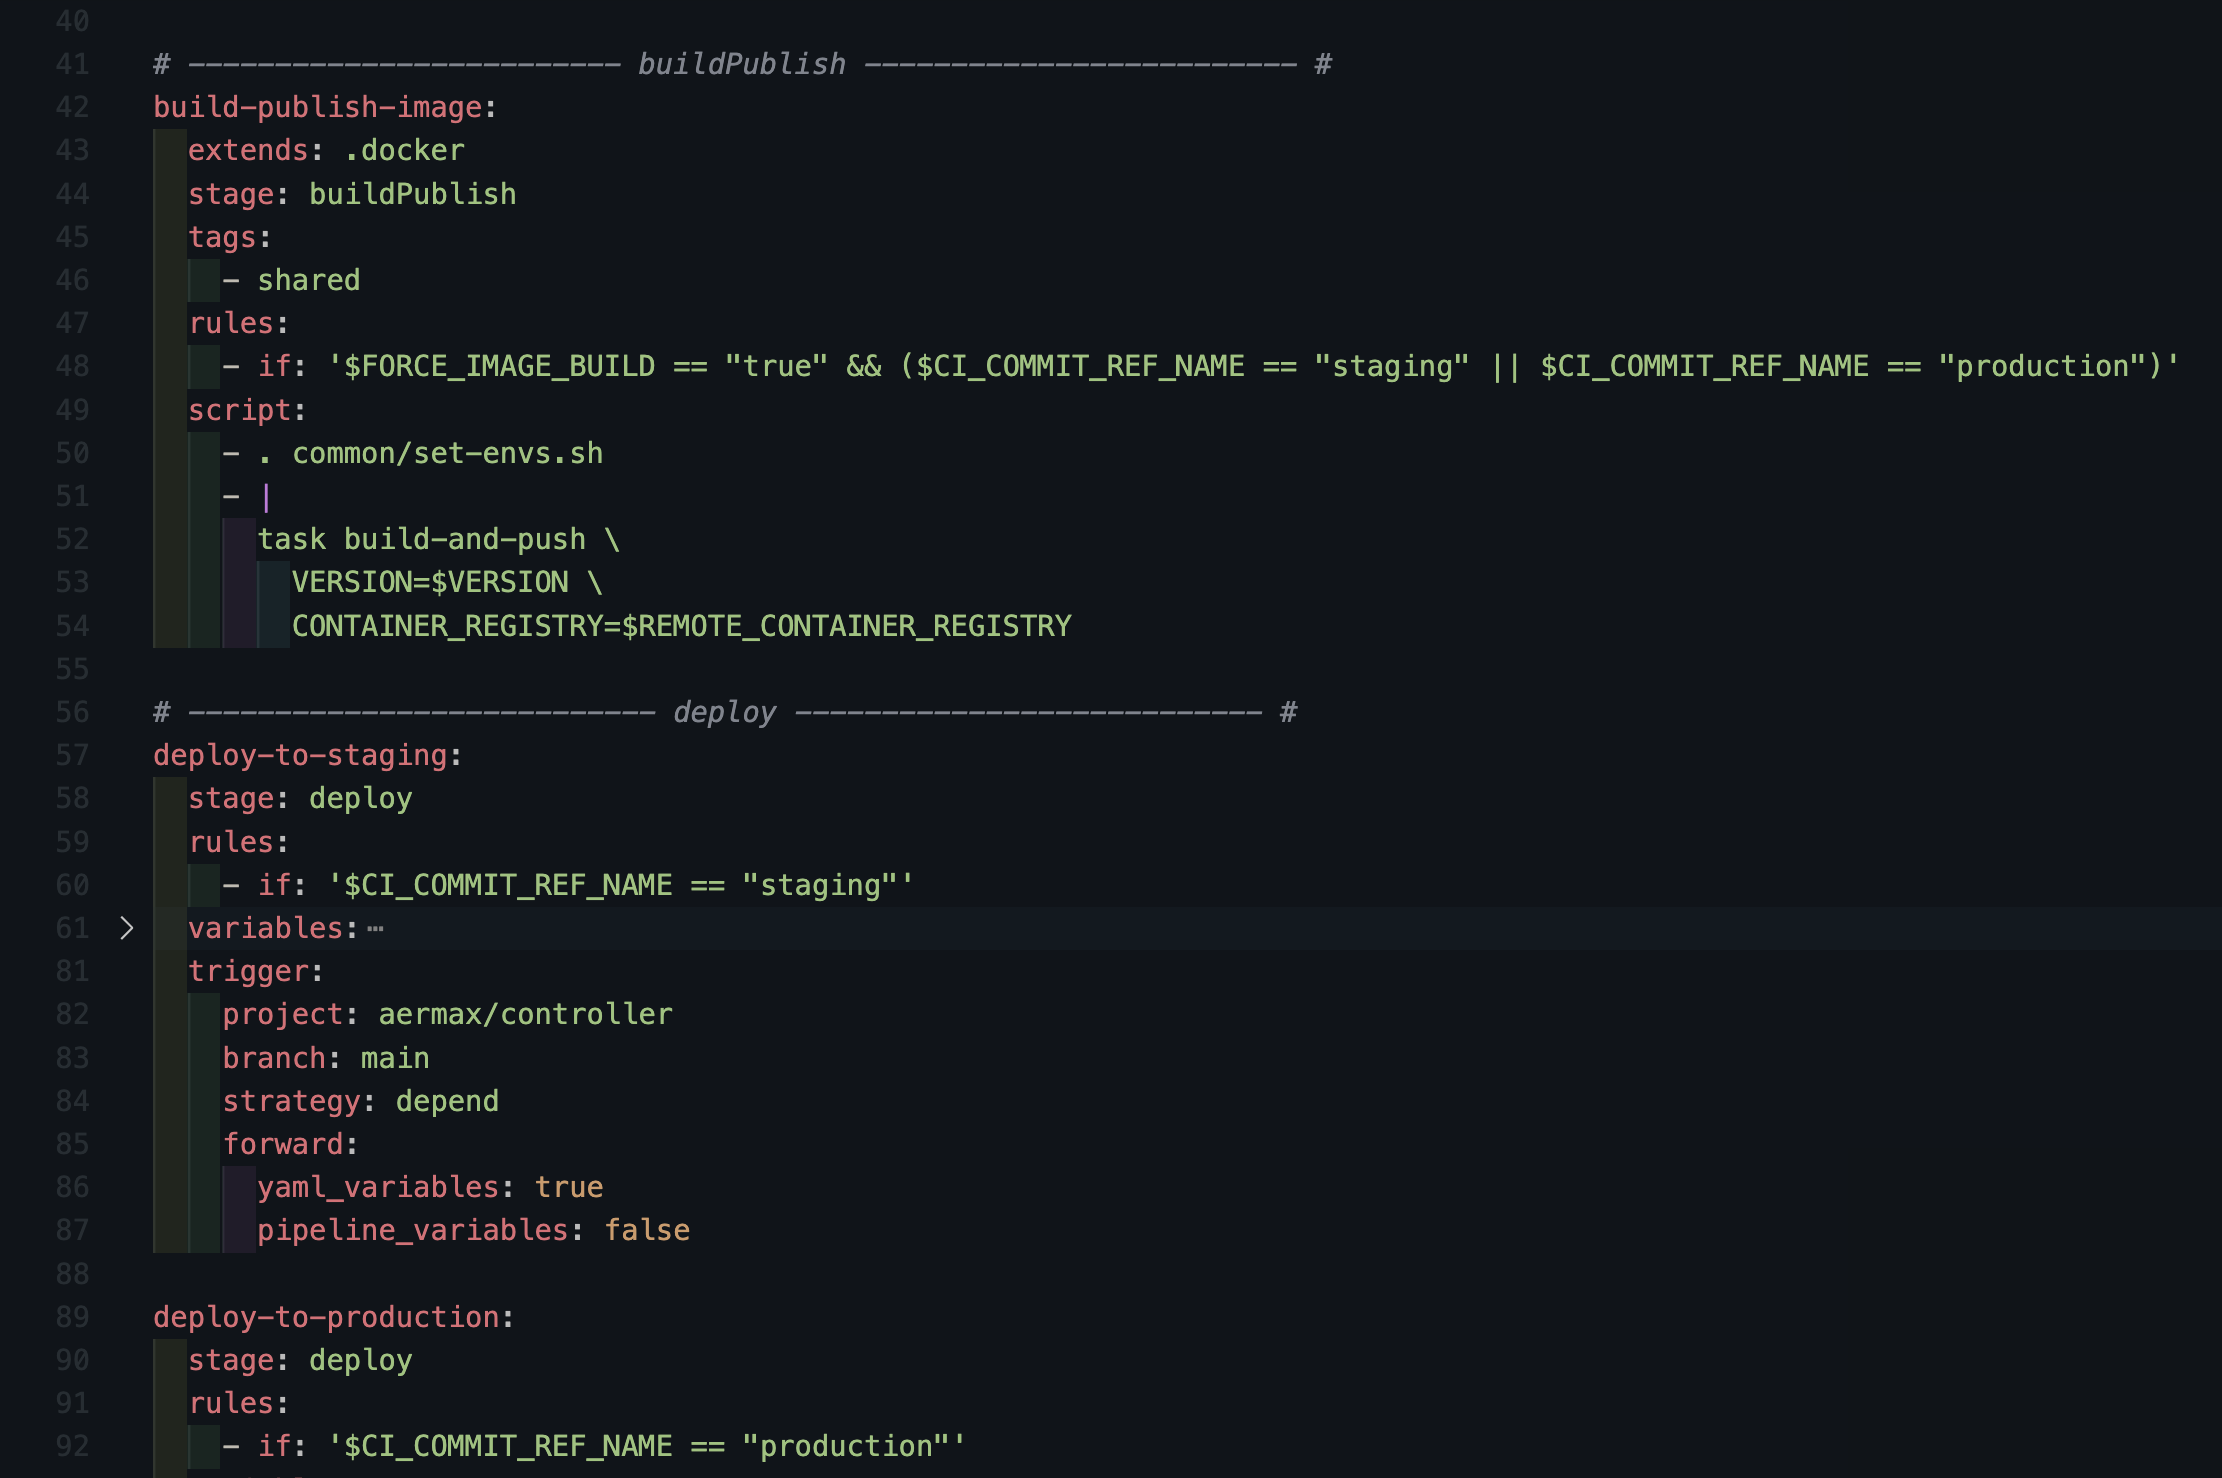
\includegraphics[width=1\textwidth]{src/assets/chapters/ci.png}
  \caption{Extract from the CI pipeline}
  \label{fig:ci-pipeline}
\end{figure}


\subsubsection{Continuous Deployment}
The aermax-controller repository, which configures the agent, selects the appropriate microservice for deployment based on the trigger input. It proceeds to configure the required environment variables and deploys it using a customized Helm package designed for this purpose.


\begin{figure}[H]
  \centering
  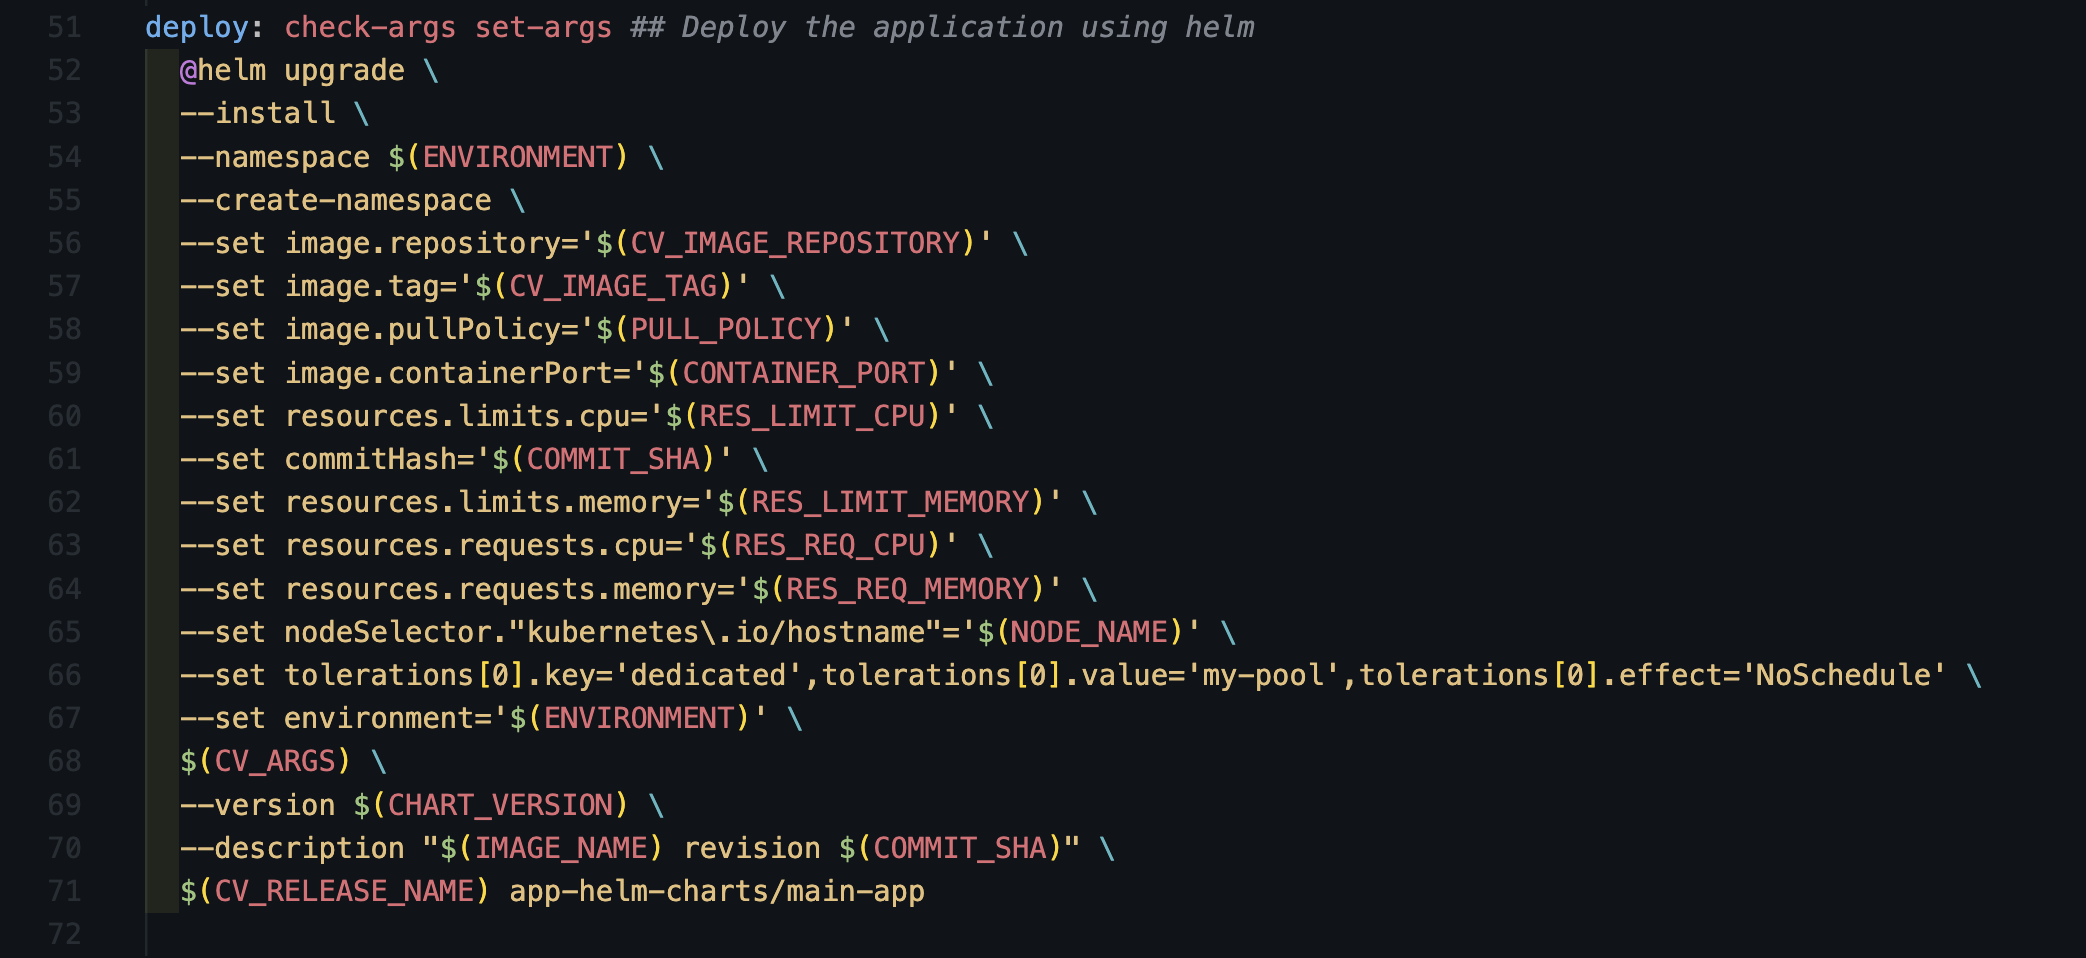
\includegraphics[width=1\textwidth]{src/assets/chapters/cd.png}
  \caption{Extract from the deployment Makefile}
  \label{fig:cd-pipeline}
\end{figure}


\subsubsection{Custom Helm Package}
After deciding to utilize Helm, we have developed our own package - or, in Helm terms, a chart - to handle the resources of the Kubernetes cluster.


\begin{figure}[H]
  \centering
  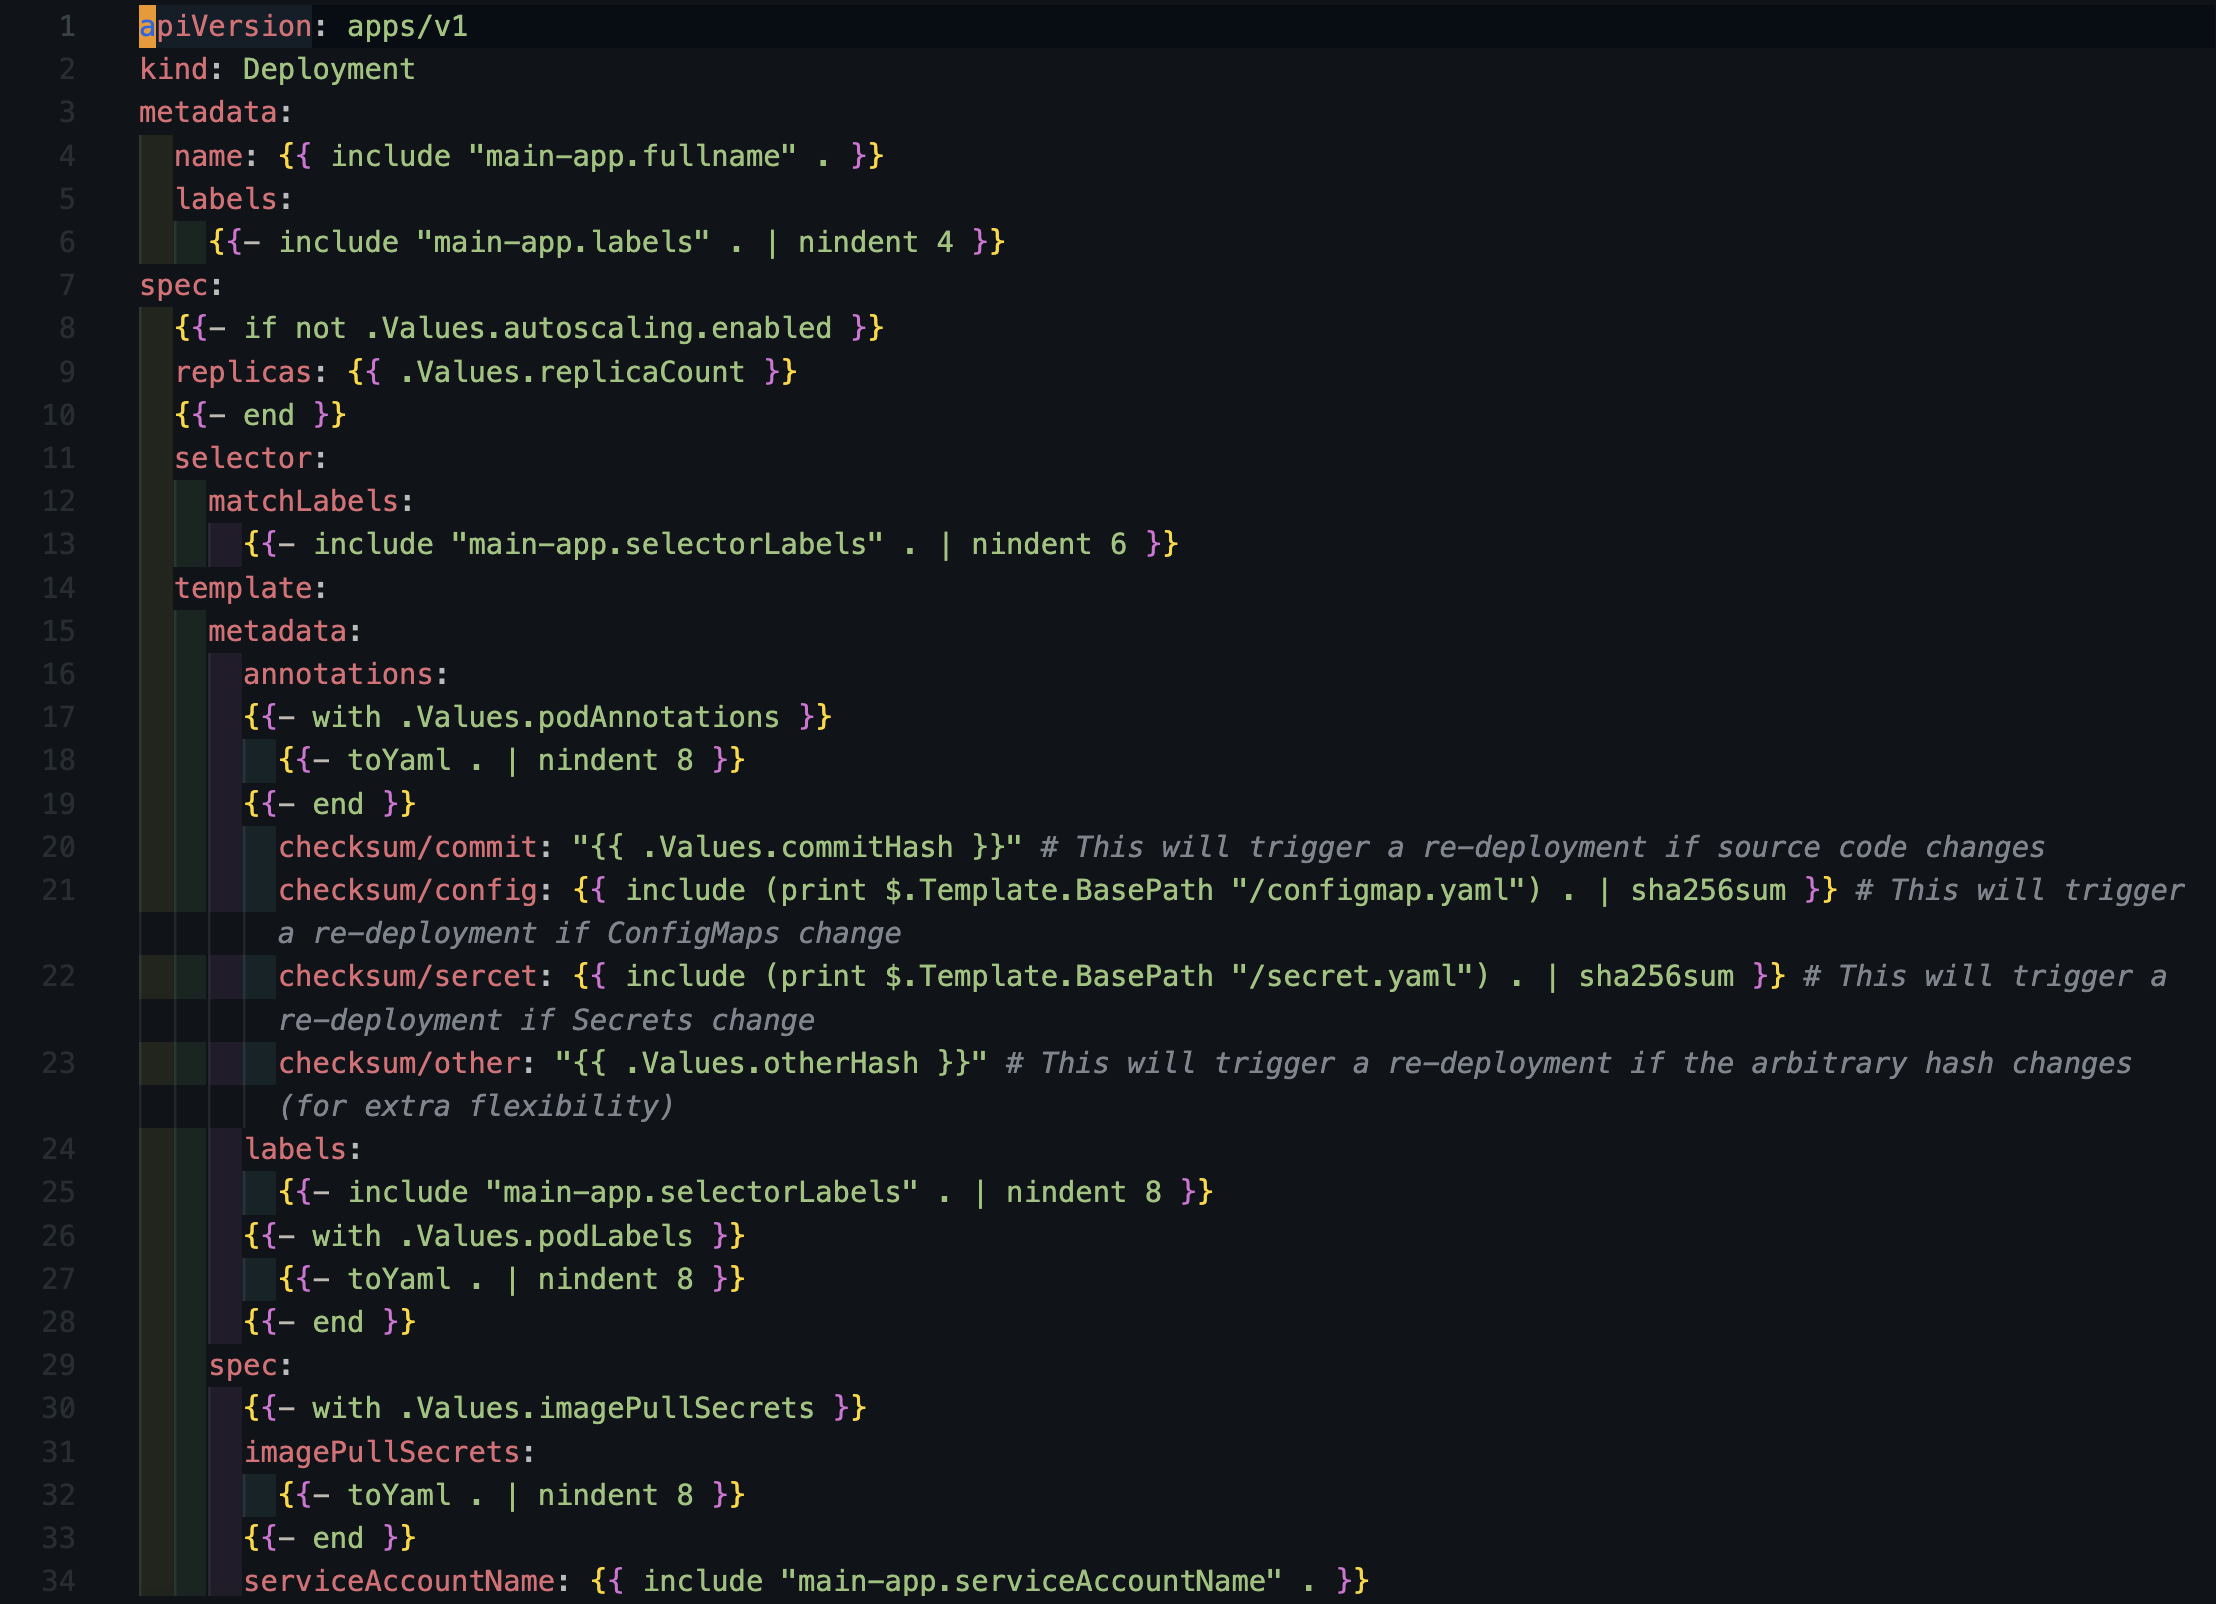
\includegraphics[width=1\textwidth]{src/assets/chapters/customhelm.png}
  \caption{Extract from the custom Helm Chart}
  \label{fig:custom-helm}
\end{figure}

The Helm Charts are customized for the CI/CD pipelines of the project to enable easy installation and upgrading of the project's application(s) without the need for a manual configuration management.

\textbf{Keep in mind:}
\begin{itemize}
  \item These charts are particularly beneficial for microservices, as they generally have a similar structure. As a result, we utilize the \textbf{main-app}  chart for all of them. However, it can still be used for a single monolithic application.
  \item You have the option to create additional charts as required using \textbf{helm create}, but it's unlikely that you'll need to do so.
  \item this chart does not contain any ingress rules. You will still need to apply those manually from the common manifest in the controller. This approach simplifies the process of identifying exposed domains without the need to redeploy all releases separately.

\end{itemize}


\begin{figure}[H]
  \centering
  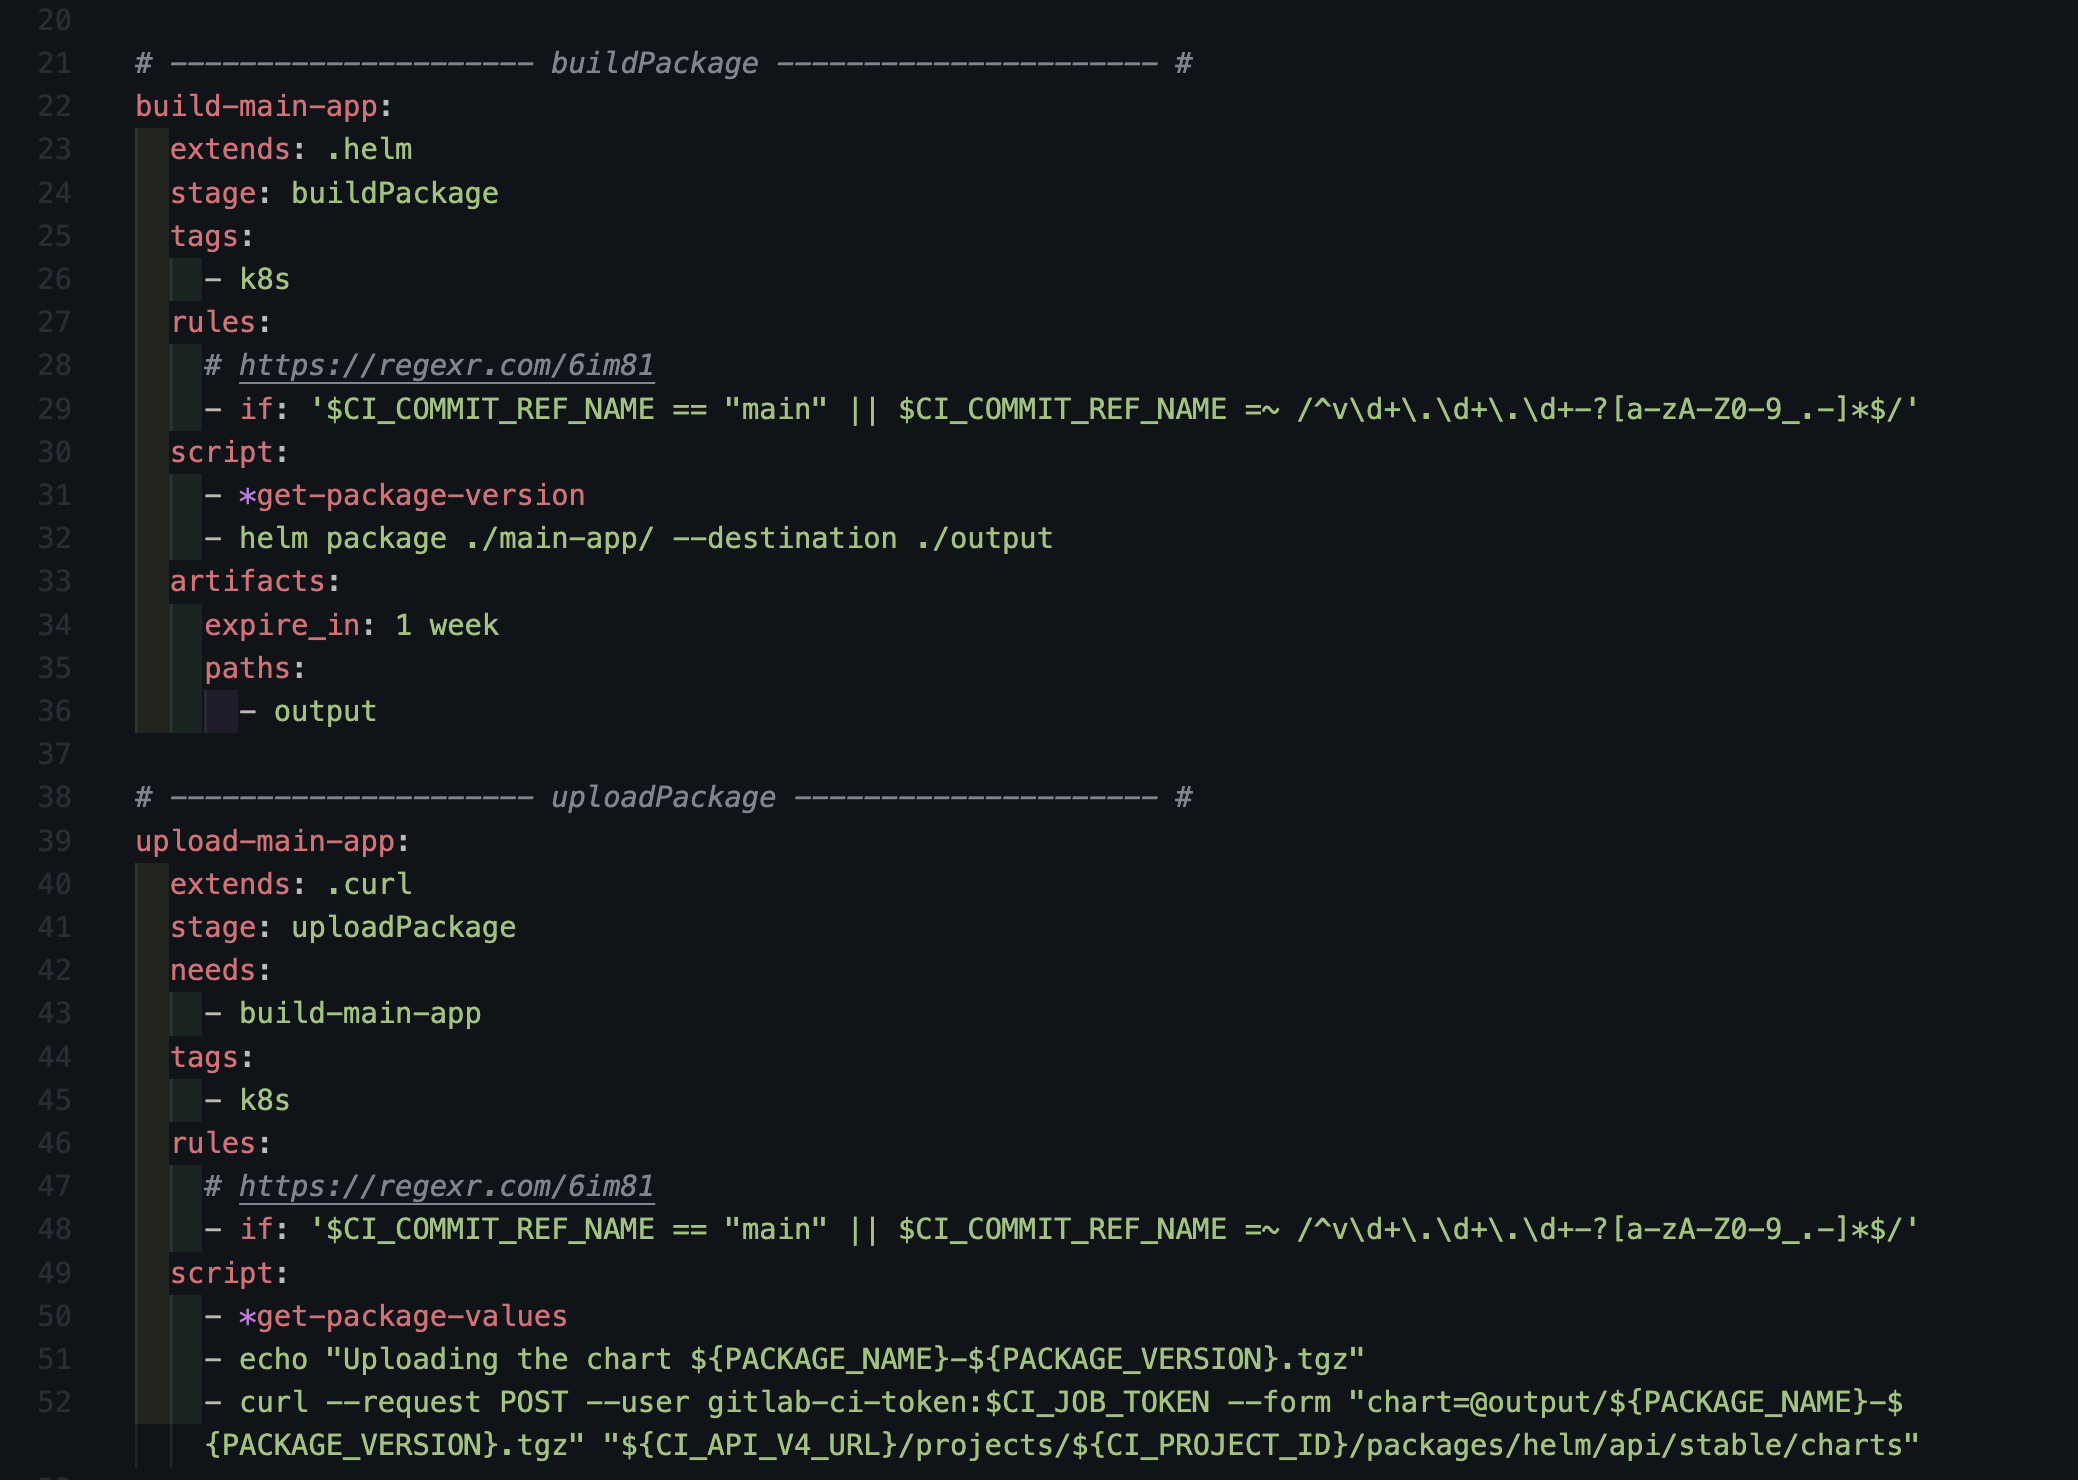
\includegraphics[width=1\textwidth]{src/assets/chapters/helmpipeline.png}
  \caption{Extract from the custom Helm package’s pipeline}
  \label{fig:custom-helm-pipeline}
\end{figure}

\subsubsection{Deployment result}
And if we trigger the CI/CD pipeline for all our microservices (refer to Appendix C), we will be able to observe the deployment of the application dashboard! As a matter of fact, we currently have two active environments that are accessible to the public:

\begin{itemize}
  \item \textbf{Staging} https://staging.app.aermax.de/
  \item \textbf{Production} https://app.aermax.de/

\end{itemize}


\begin{figure}[H]
  \centering
  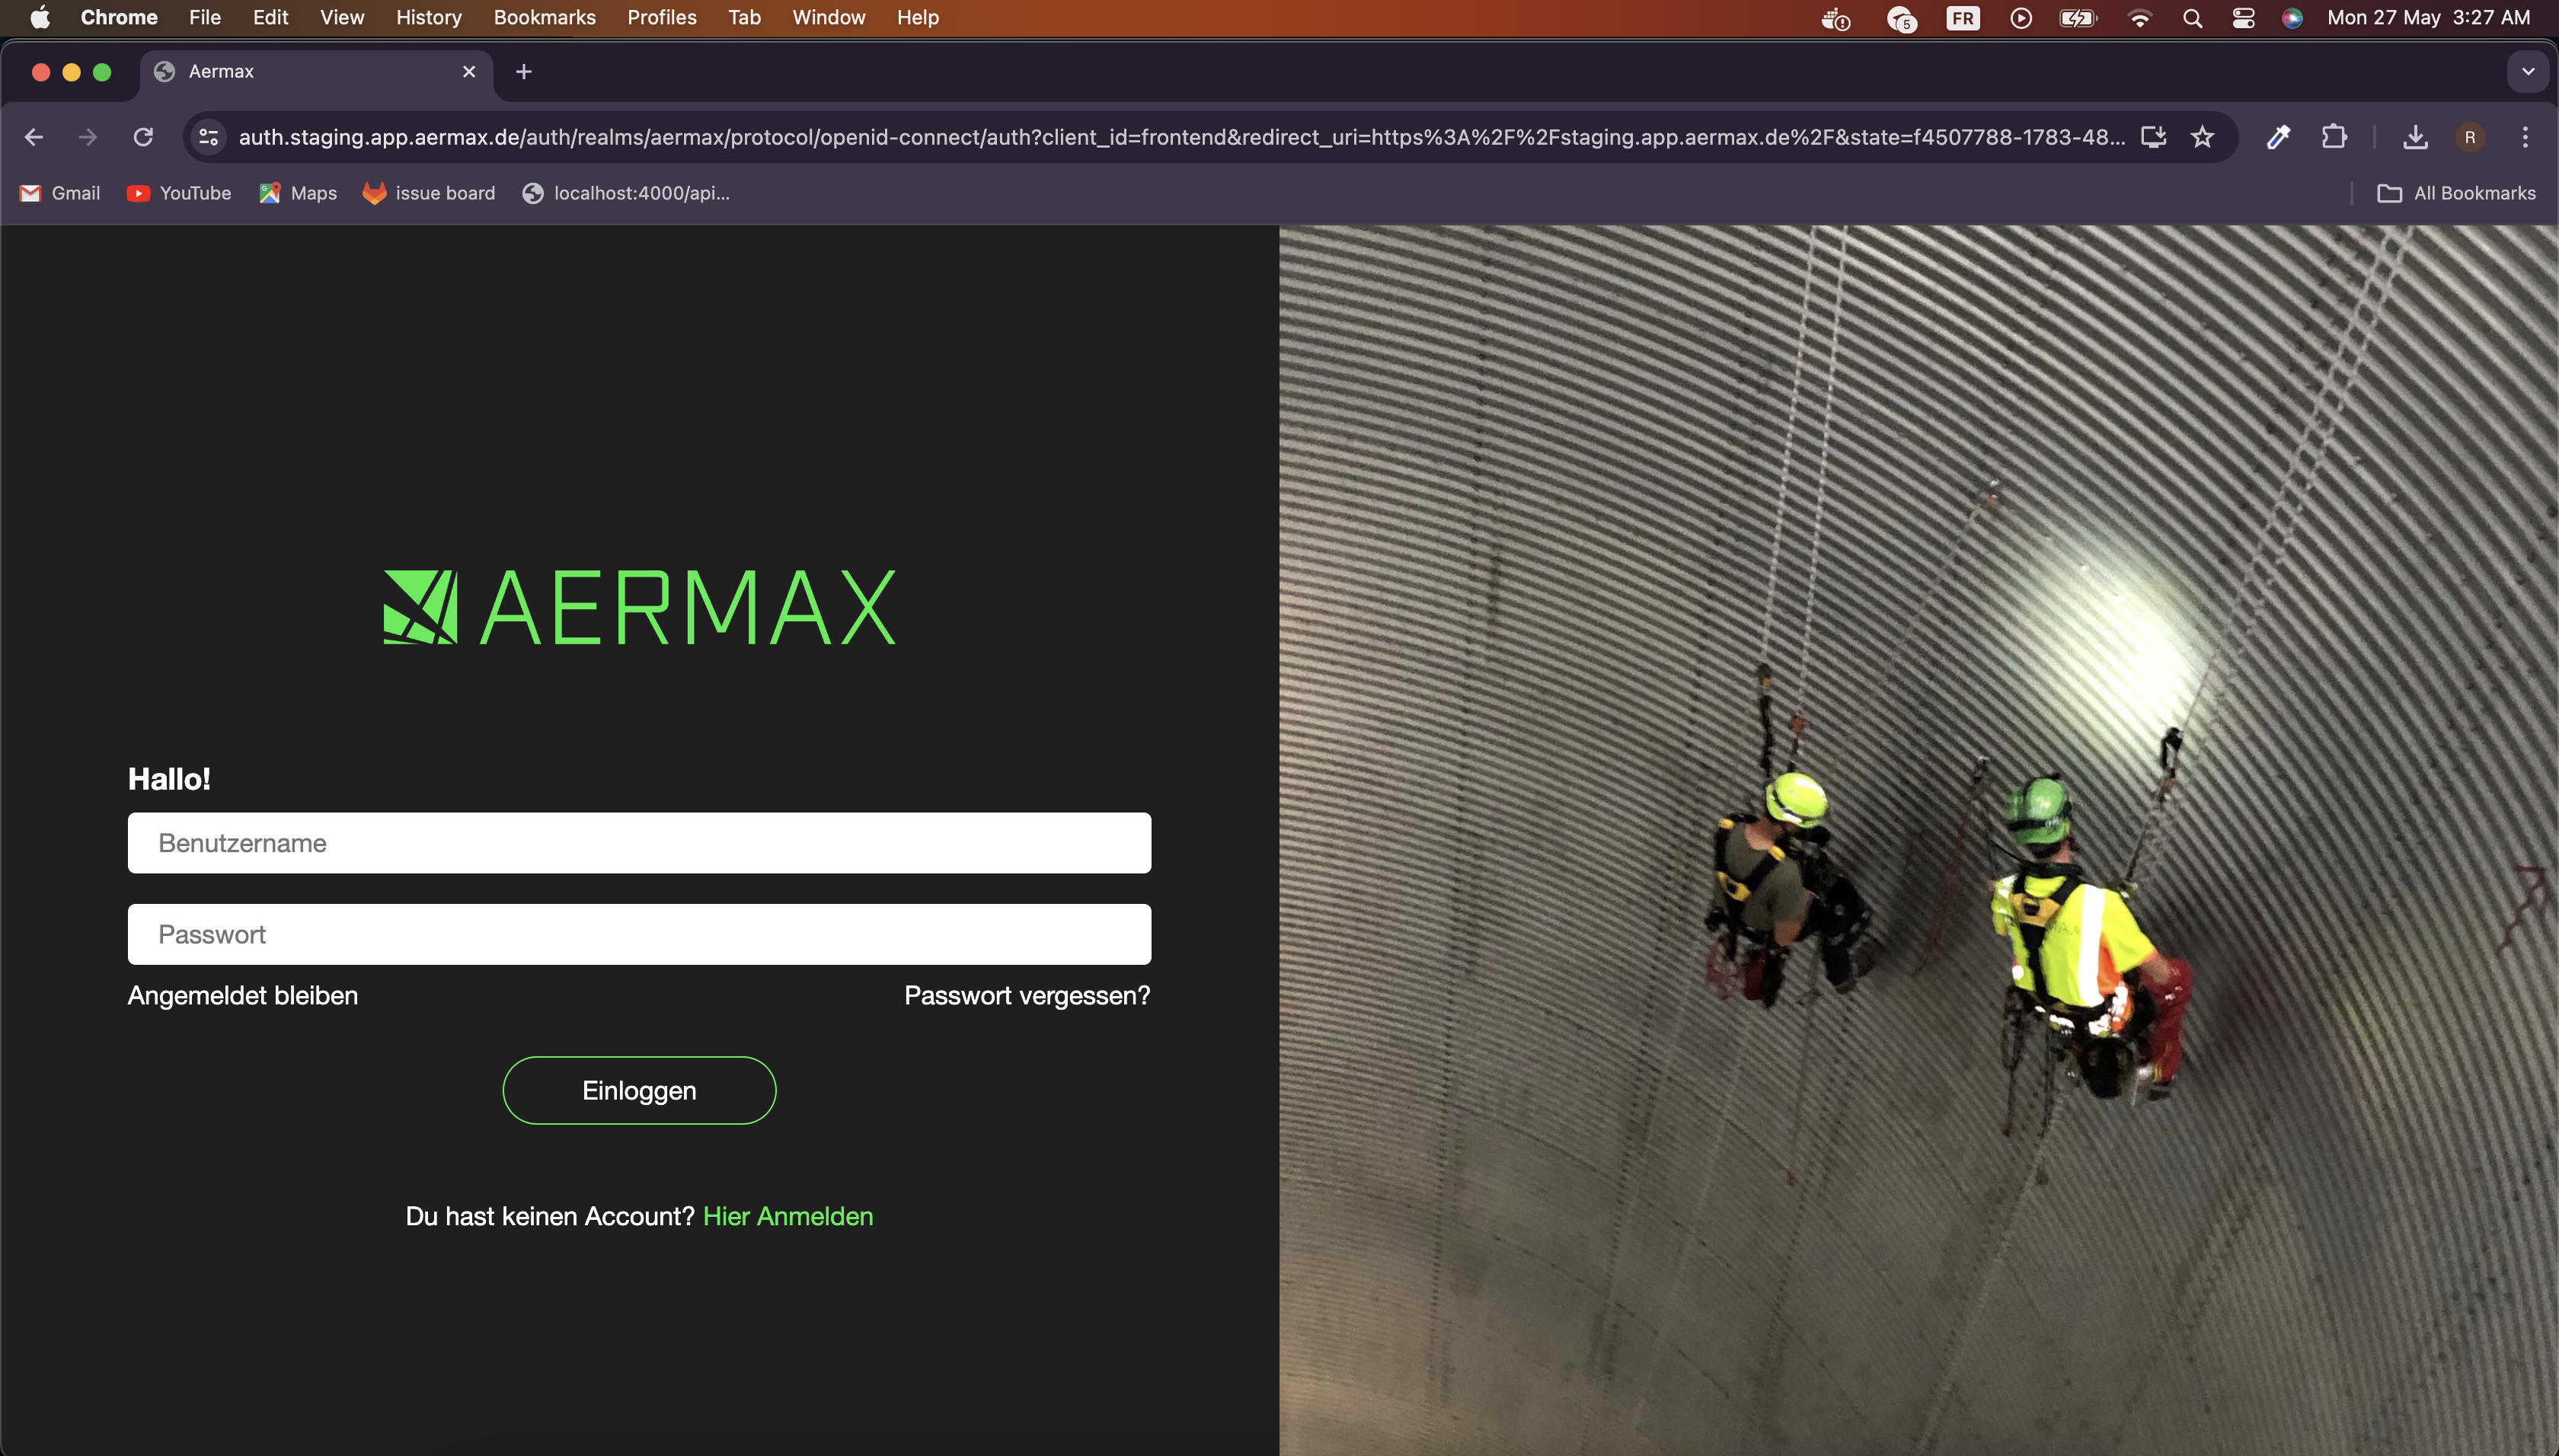
\includegraphics[width=1\textwidth]{src/assets/chapters/login.png}
  \caption{Aermax Login Page}
  \label{fig:login}
\end{figure}

When we login as admin, the dashboard with the list of projects, users, working pakets is the first thing
we notice. We can see how many in progress projects we have and
also some other useful information for admins.
We will focus just on the rewars system features.

\begin{figure}[H]
  \centering
  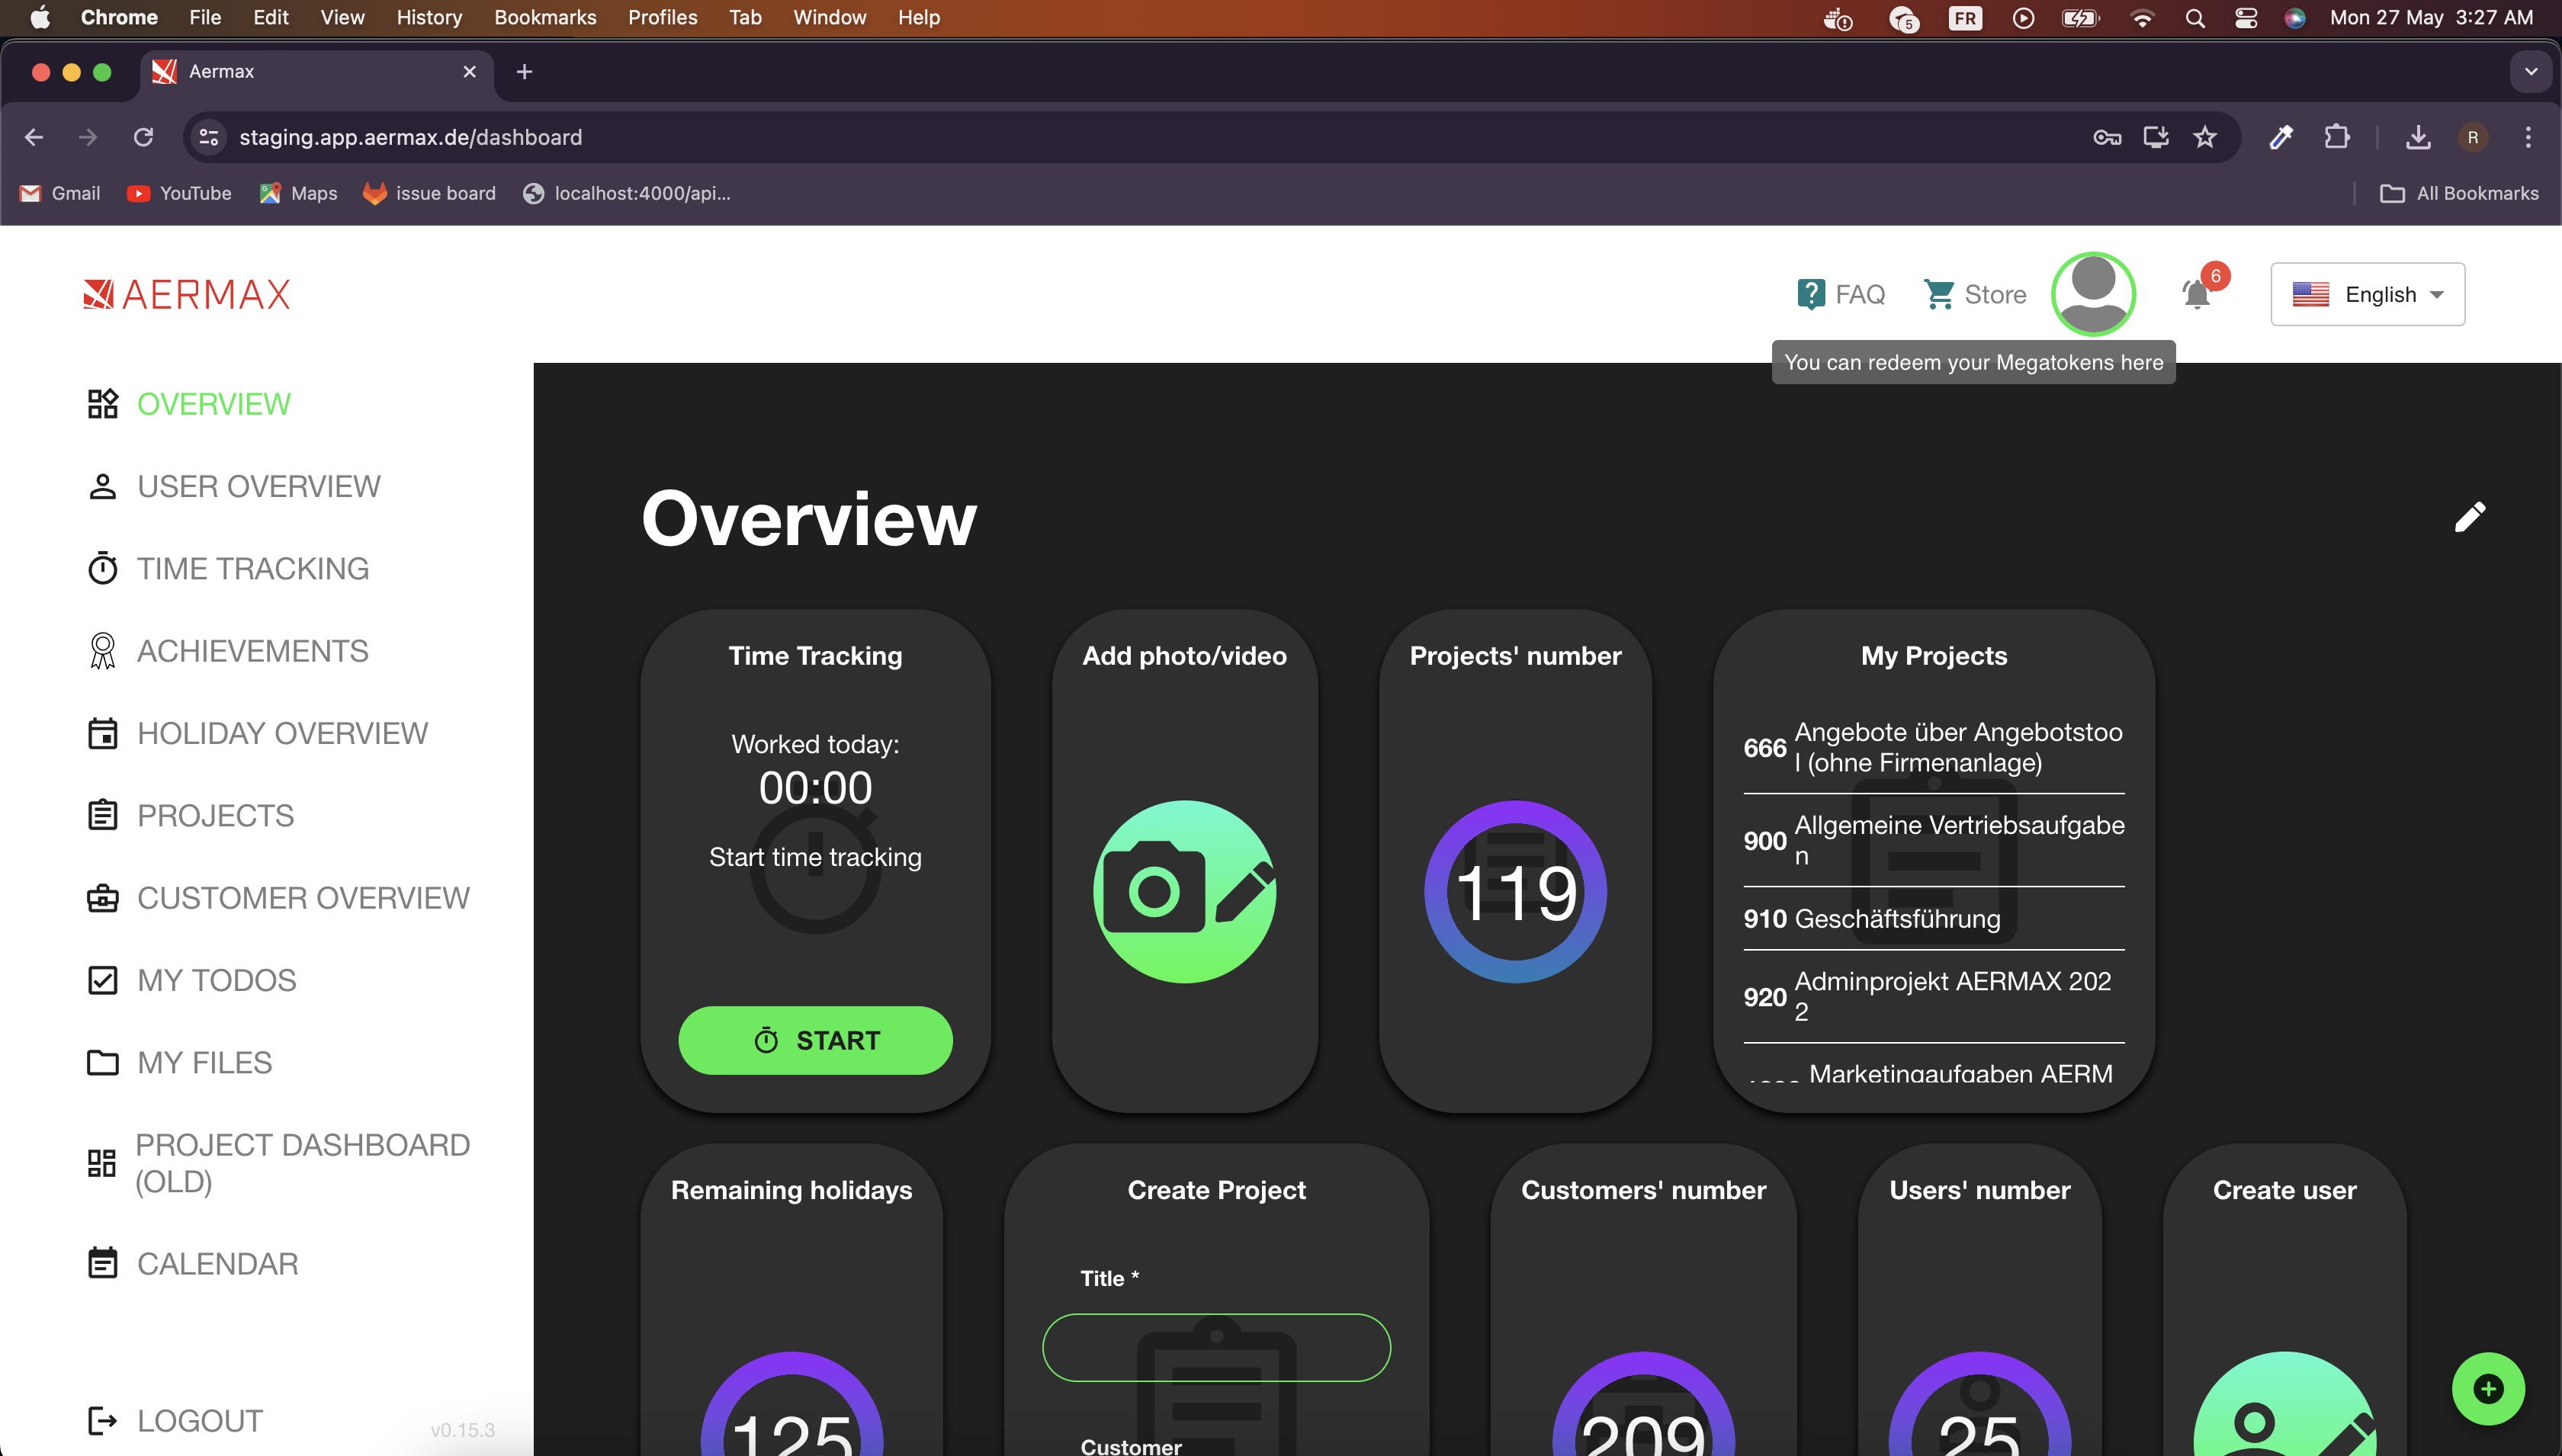
\includegraphics[width=1\textwidth]{src/assets/chapters/adminOverview.png}
  \caption{Aermax Admin Overview}
  \label{fig:admin-overview}
\end{figure}

\begin{figure}[H]
  \centering
  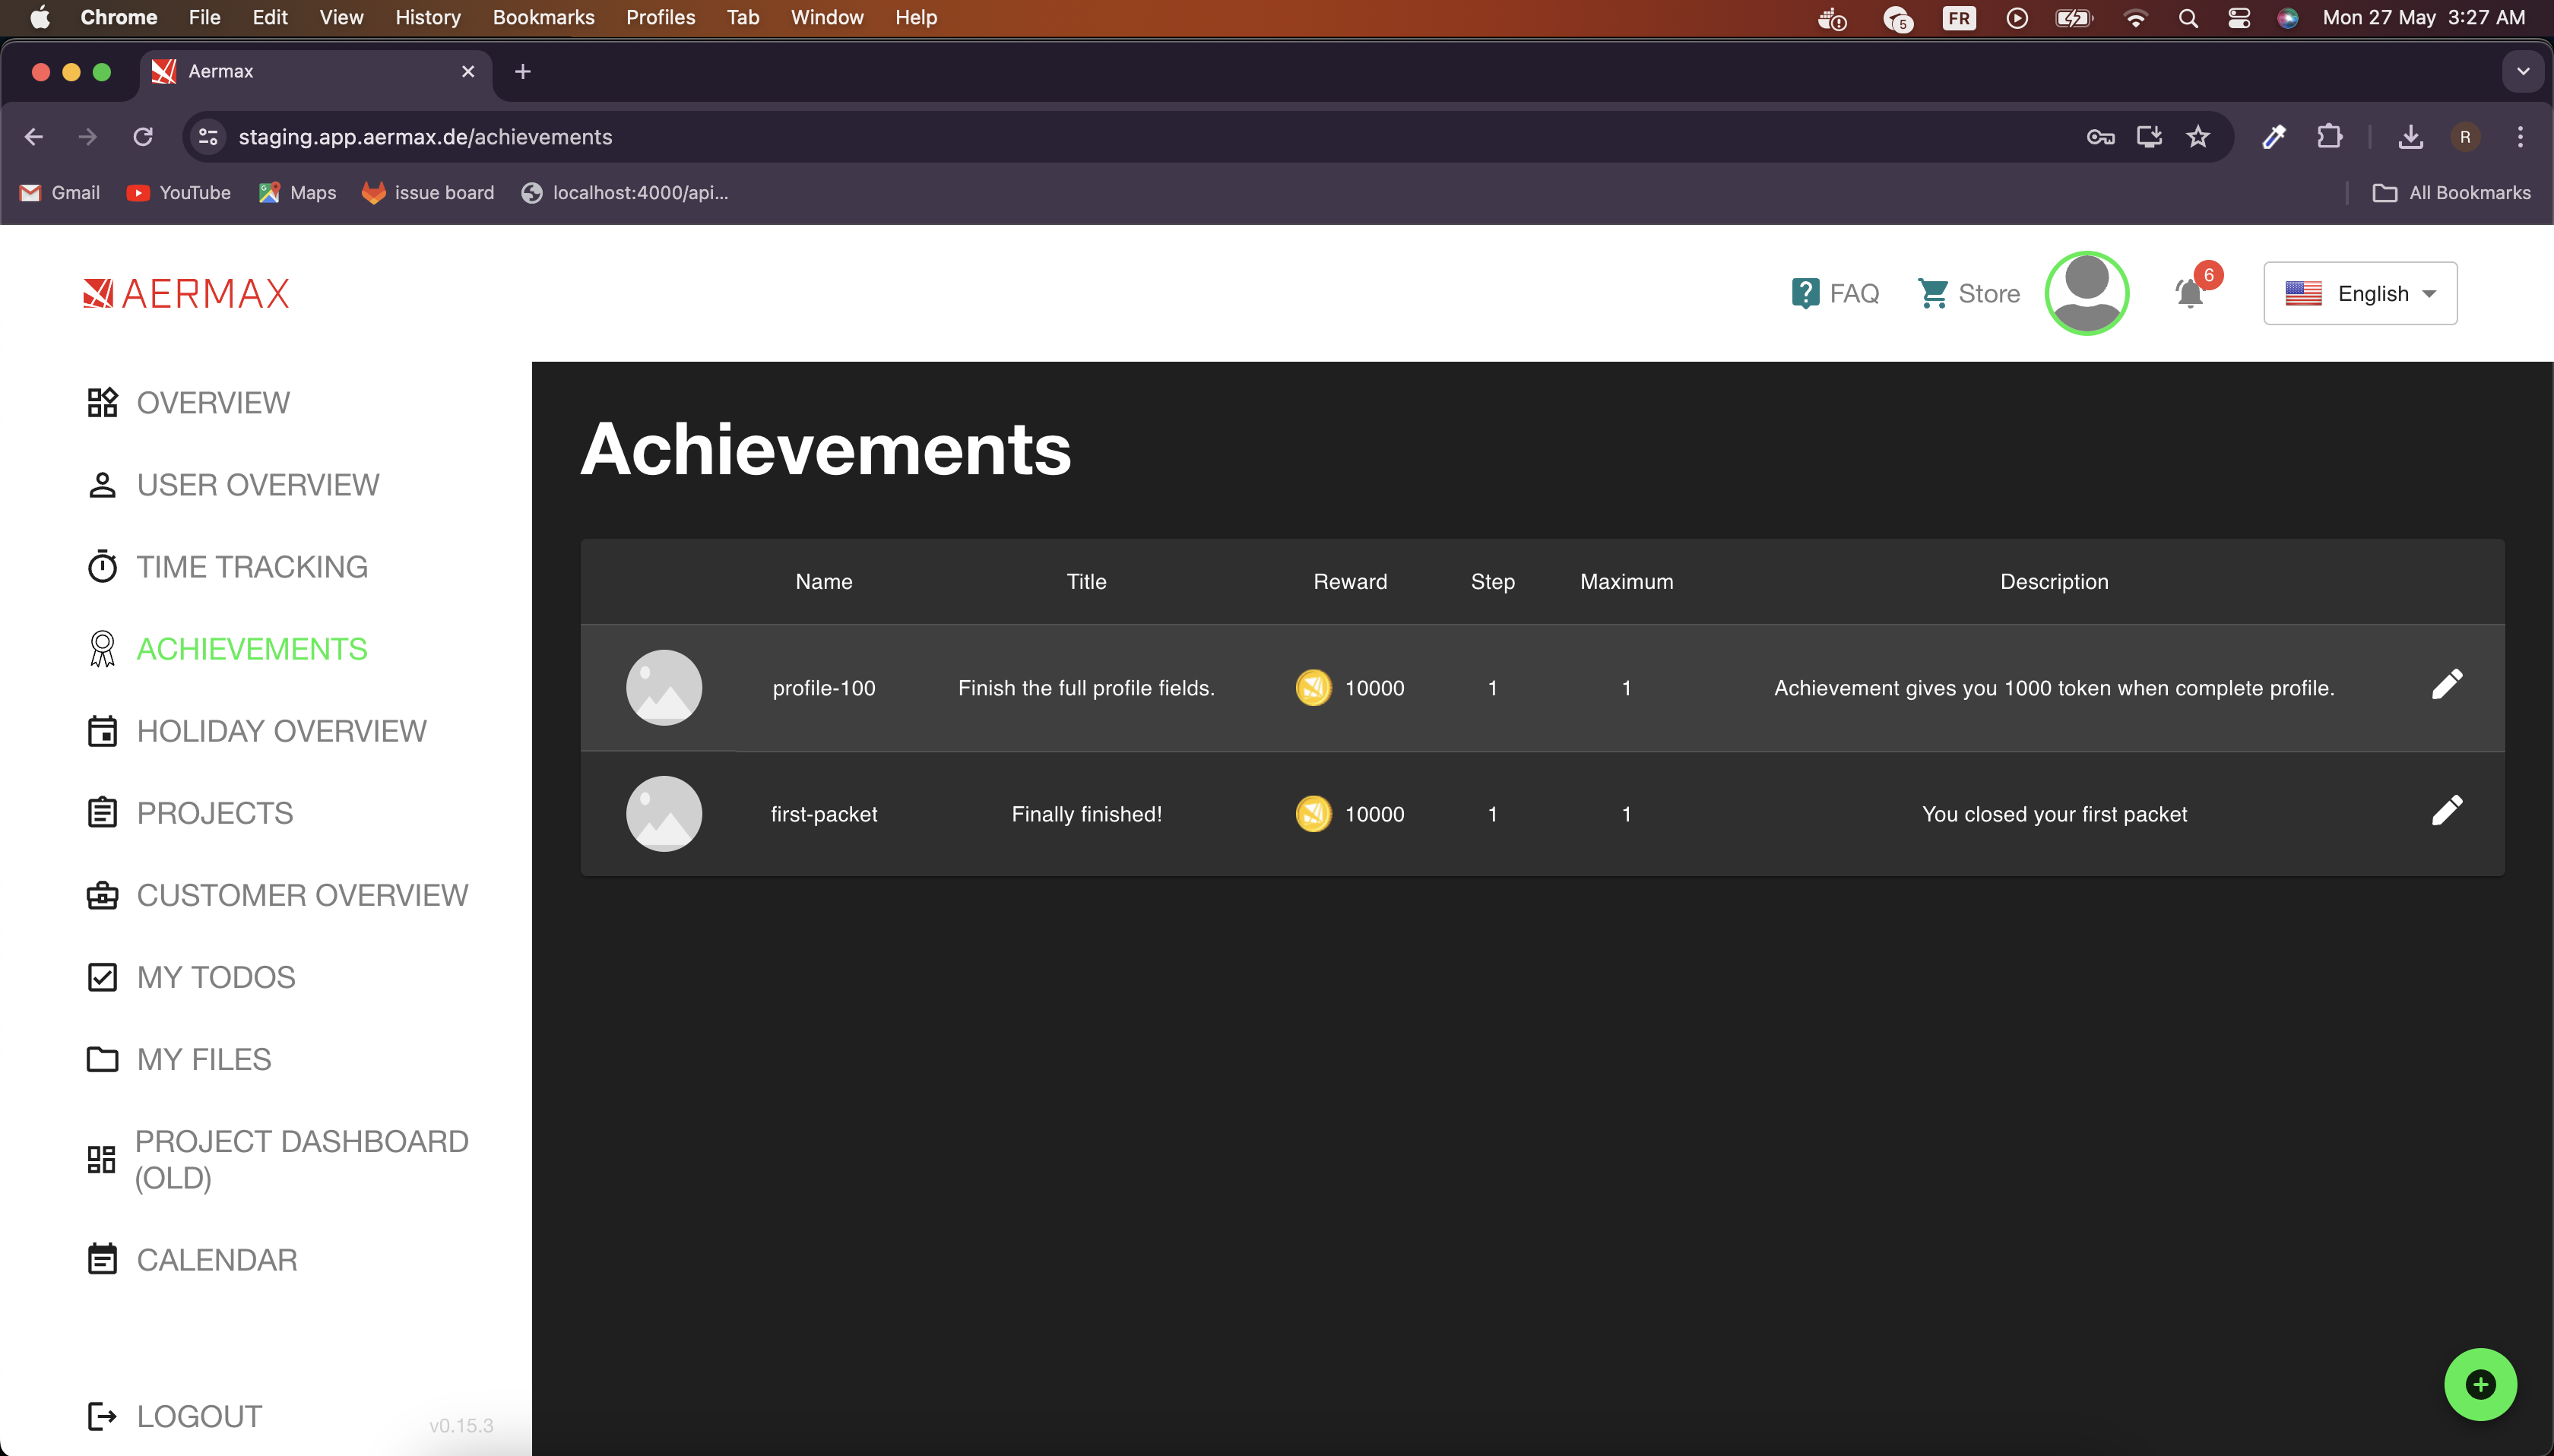
\includegraphics[width=1\textwidth]{src/assets/chapters/adminAchievements.png}
  \caption{Aermax Admin Achievements Overview}
  \label{fig:admin-achievements-overview}
\end{figure}

We additionally have the option to manage our achievements(Missions).


\begin{figure}[H]
  \centering
  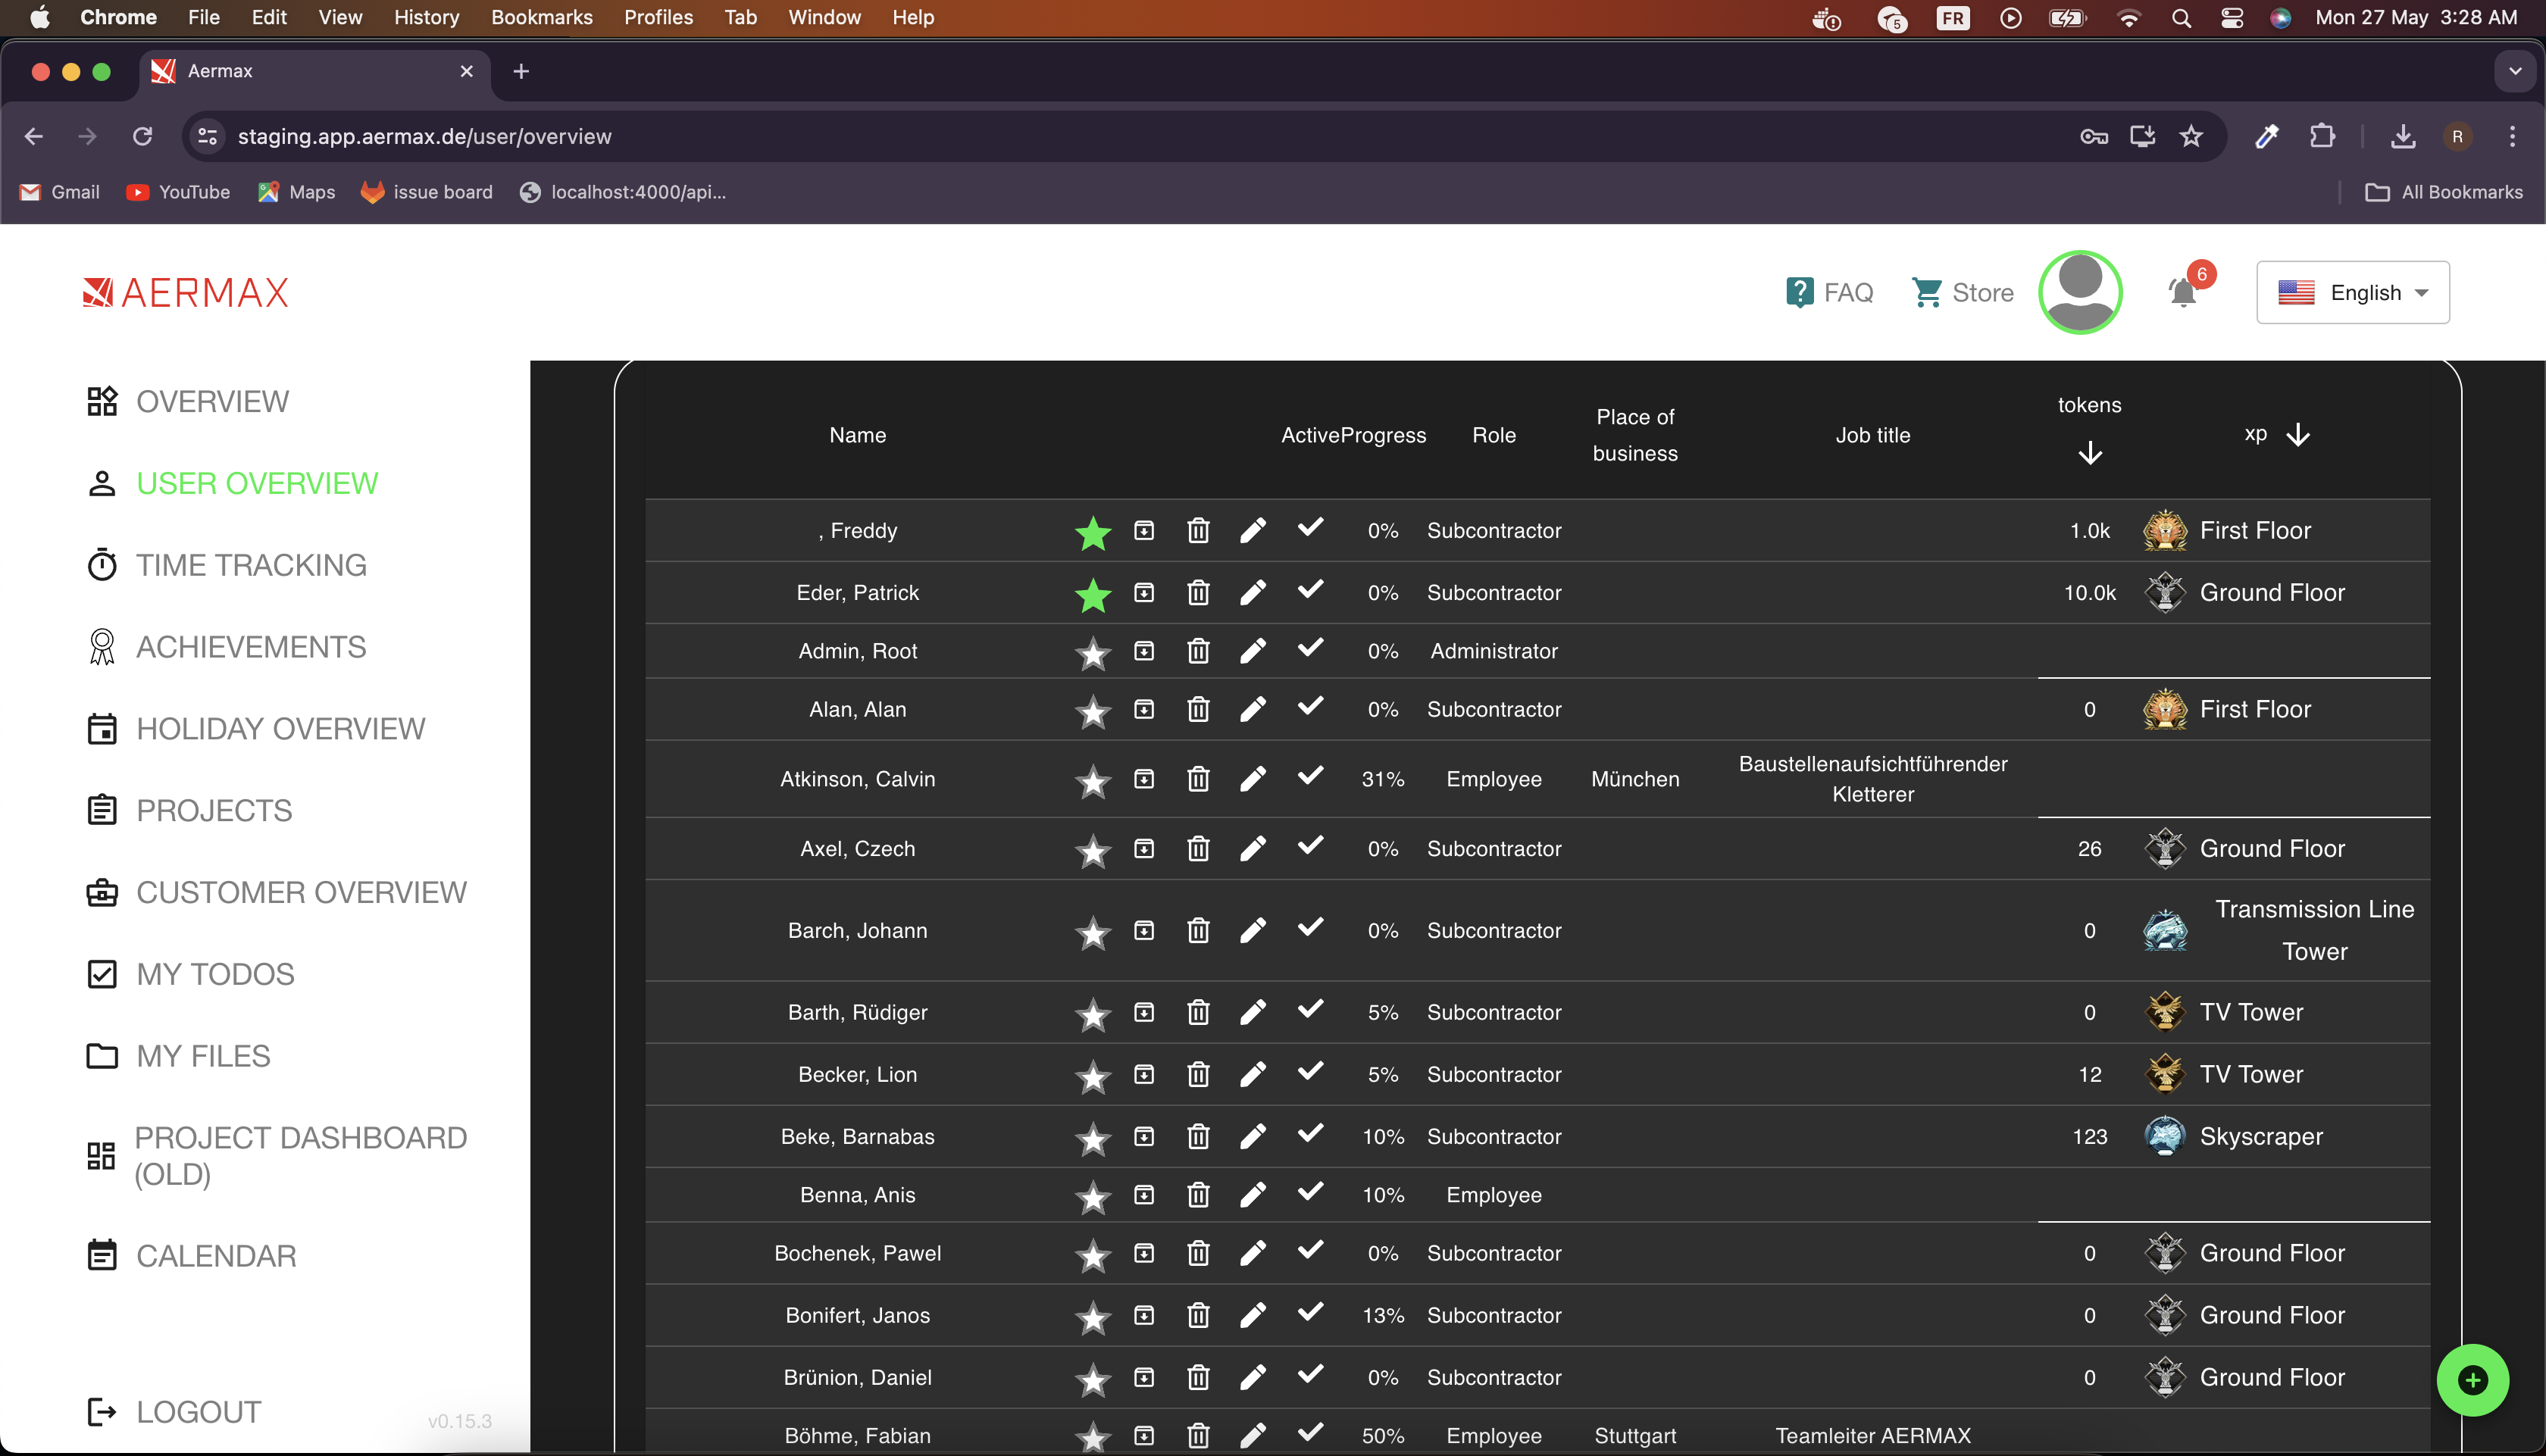
\includegraphics[width=1\textwidth]{src/assets/chapters/adminUsers.png}
  \caption{Aermax Admin Users Overview}
  \label{fig:admin-users-overview}
\end{figure}

\begin{figure}[H]
  \centering
  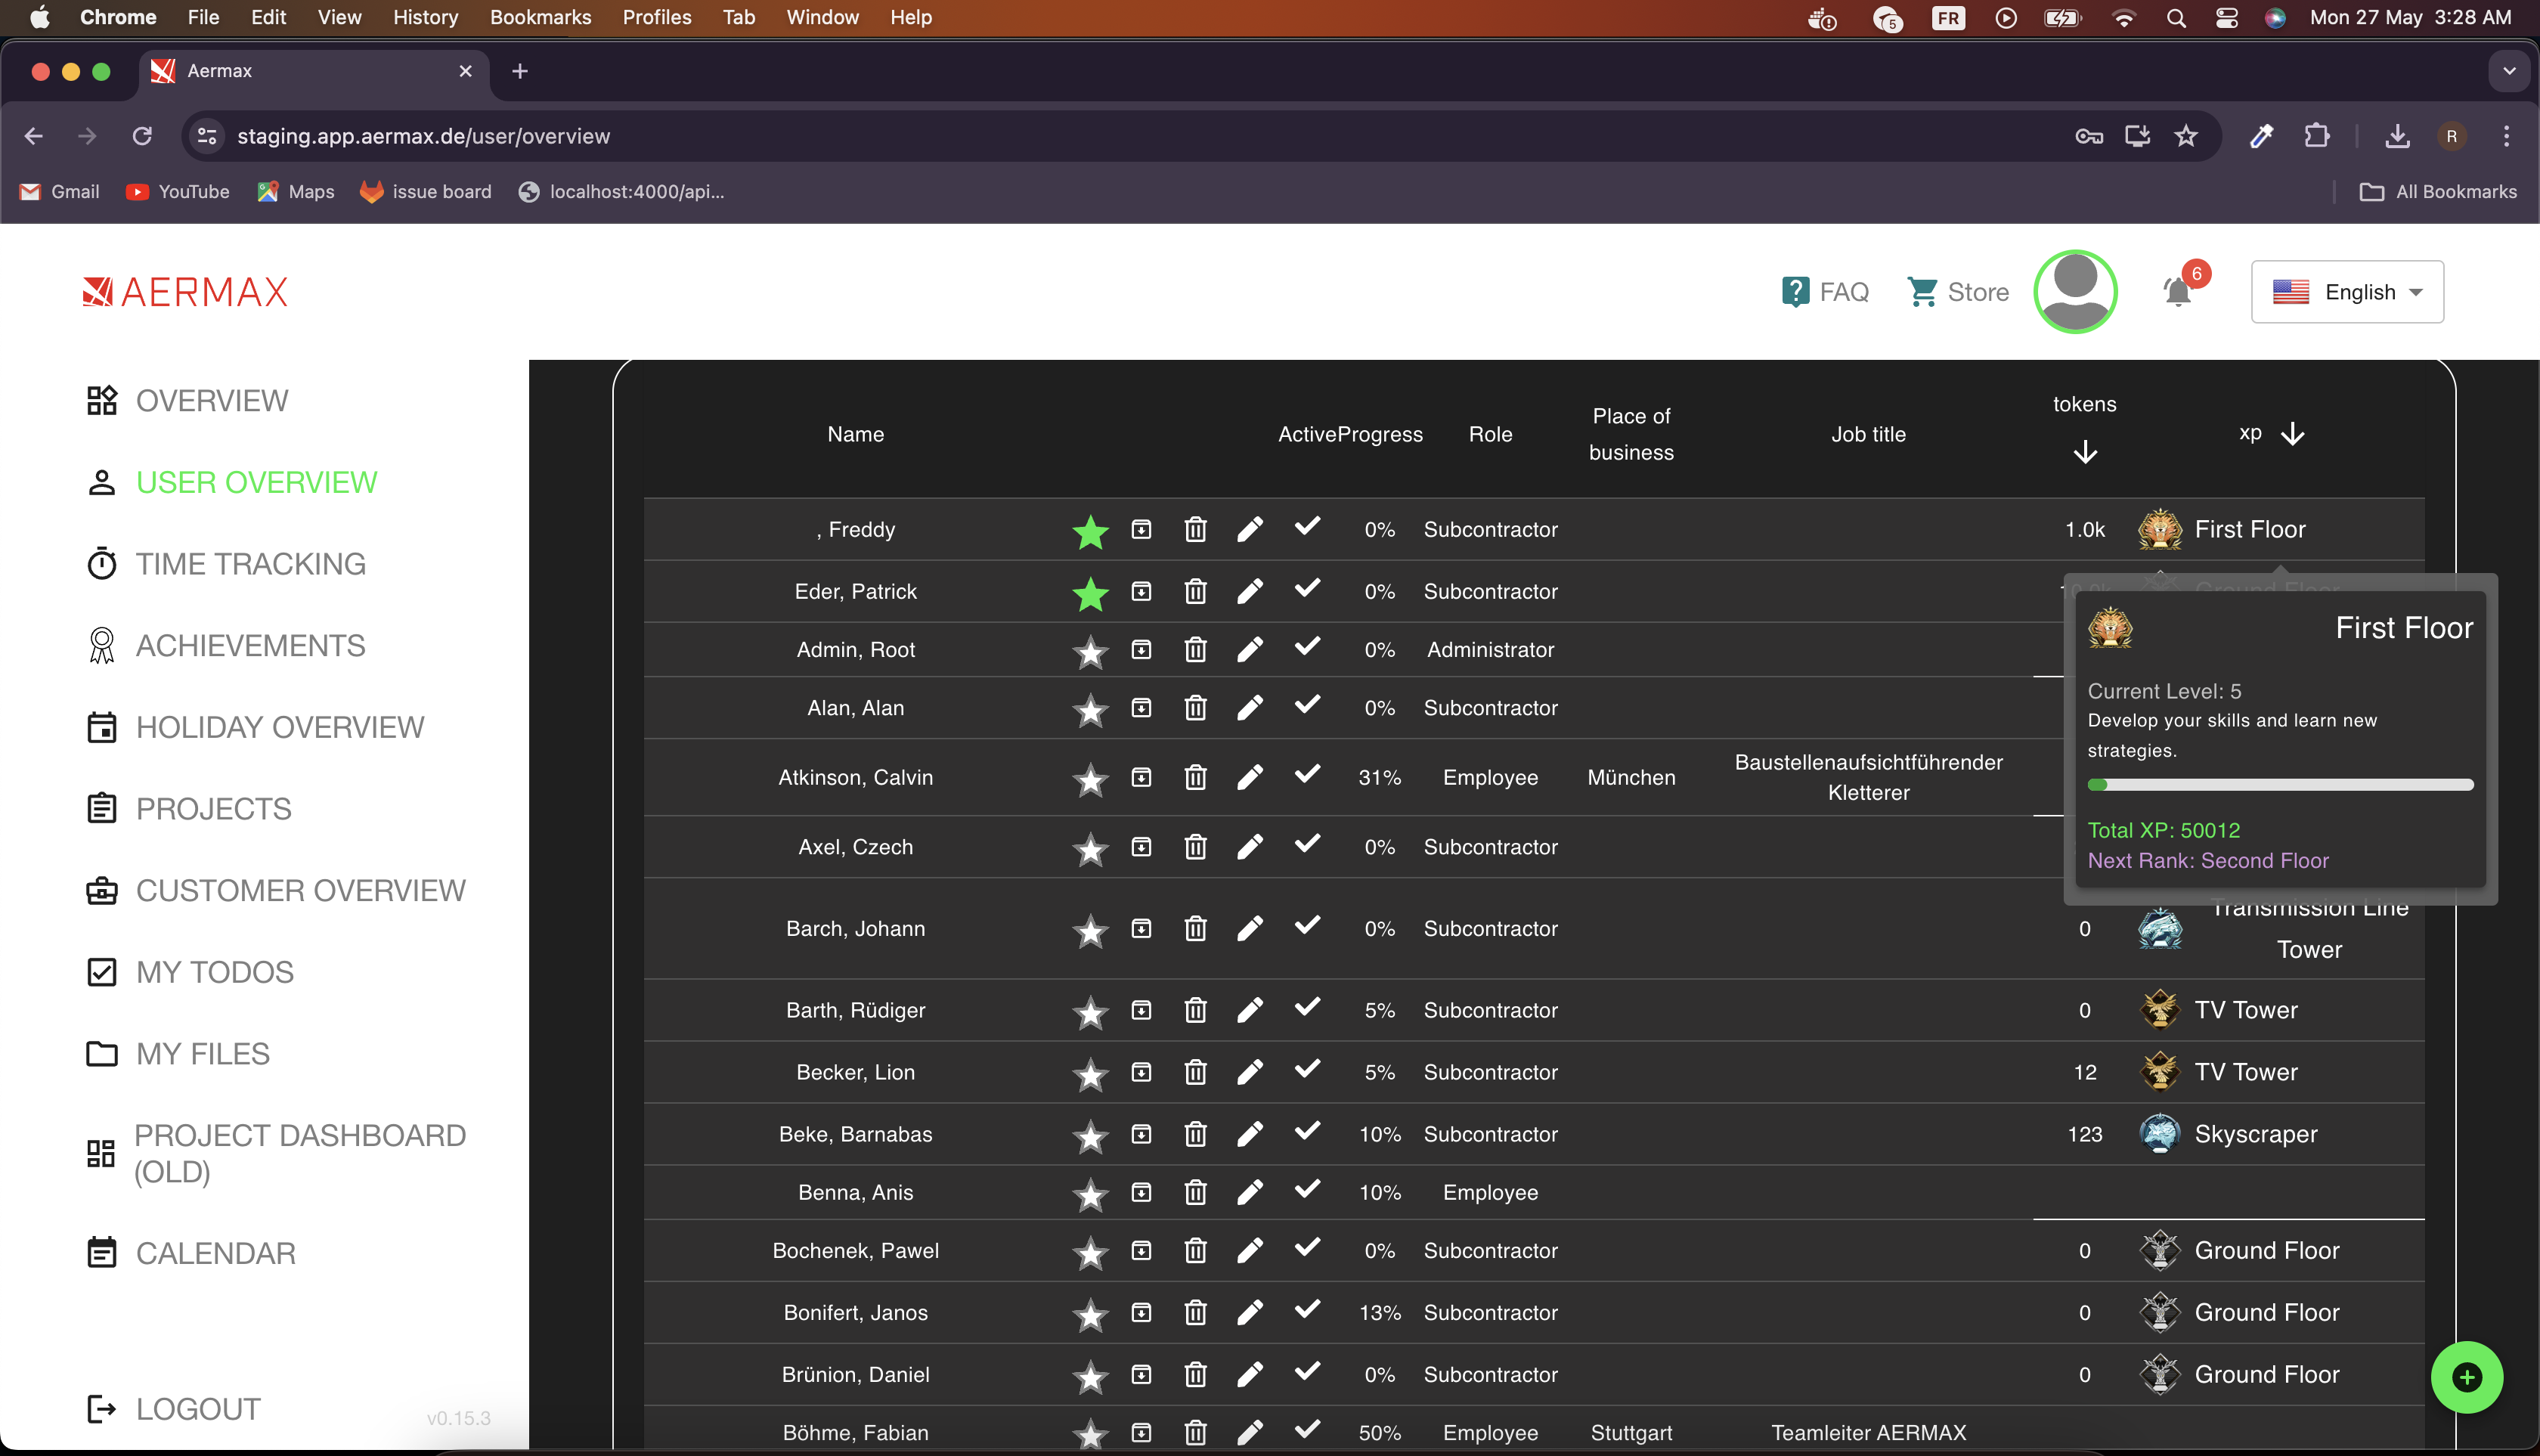
\includegraphics[width=1\textwidth]{src/assets/chapters/adminuserswithrankdetails.png}
  \caption{Aermax Admin Users Rank Details}
  \label{fig:admin-users-ranks}
\end{figure}

Admins have the option have an detailed informations about each subcompany users with navigating specifically to that user.


\begin{figure}[H]
  \centering
  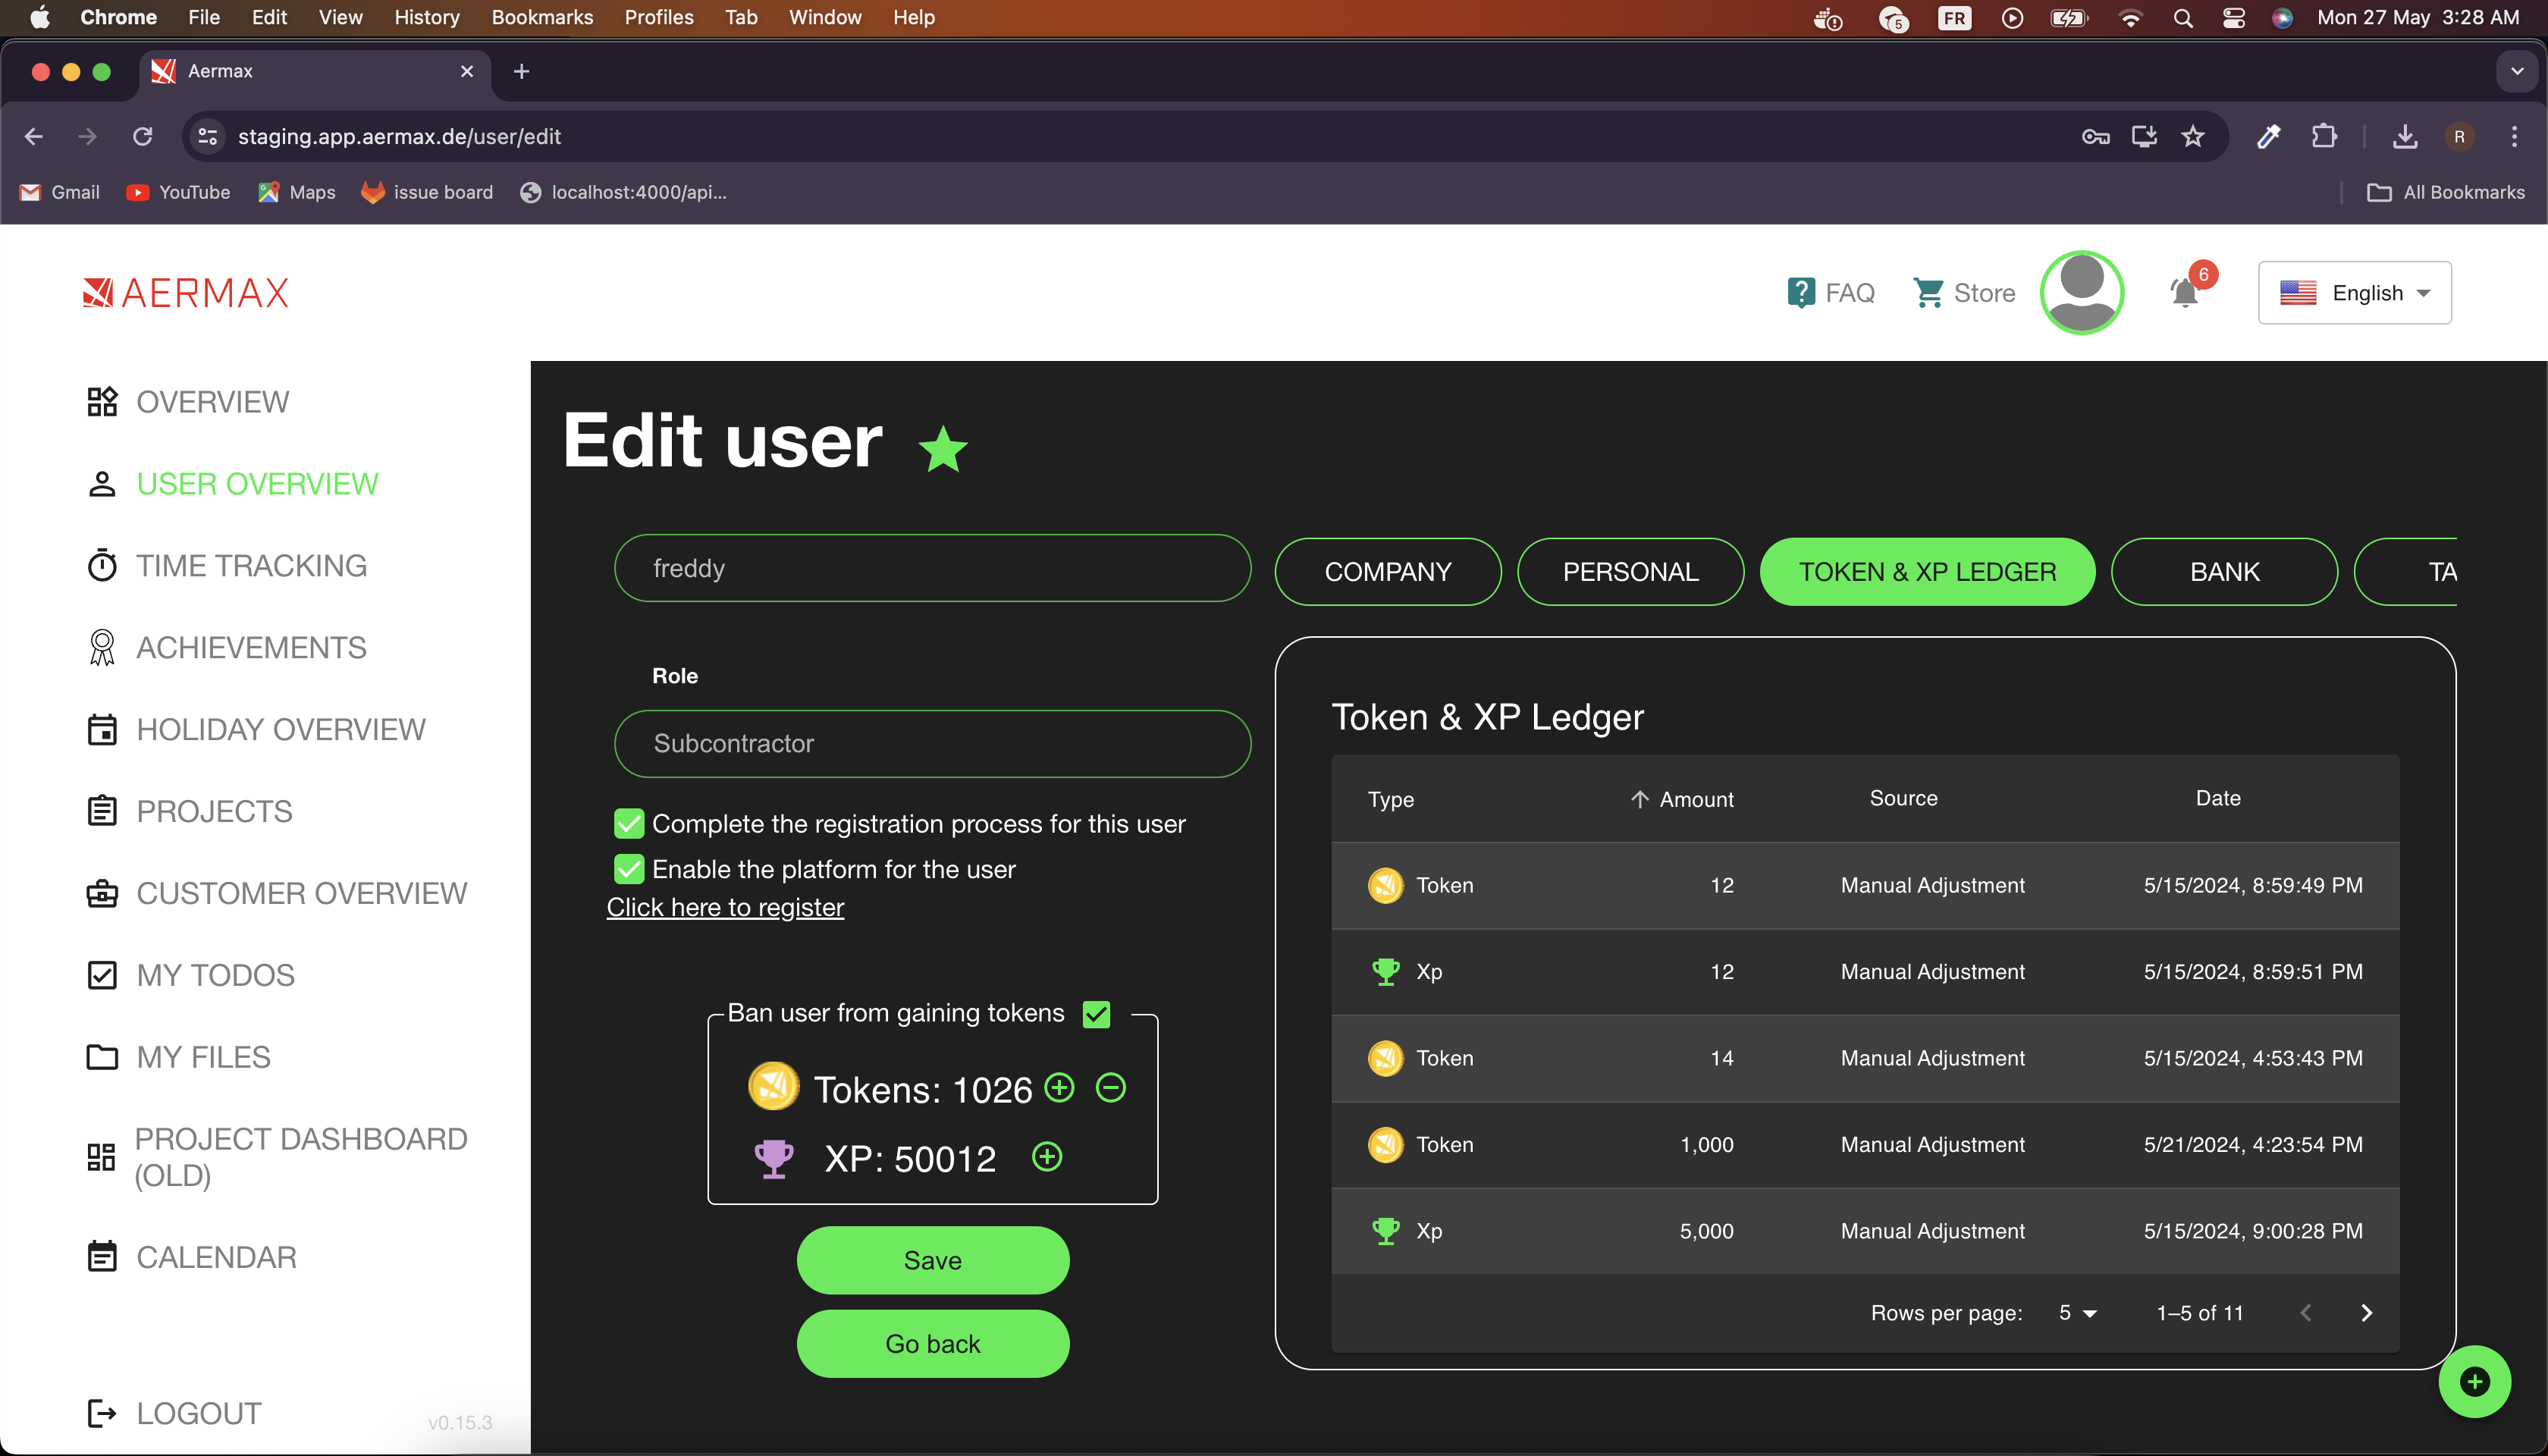
\includegraphics[width=1\textwidth]{src/assets/chapters/adminmenageranktoken.png}
  \caption{Aermax Admin Tokens Xp and Transactions Management}
  \label{fig:admin-users-tokens}
\end{figure}

Admins have the option have an detailed informations about each token and xp Transaction, with the opportunity to manage them(add/remove).


\begin{figure}[H]
  \centering
  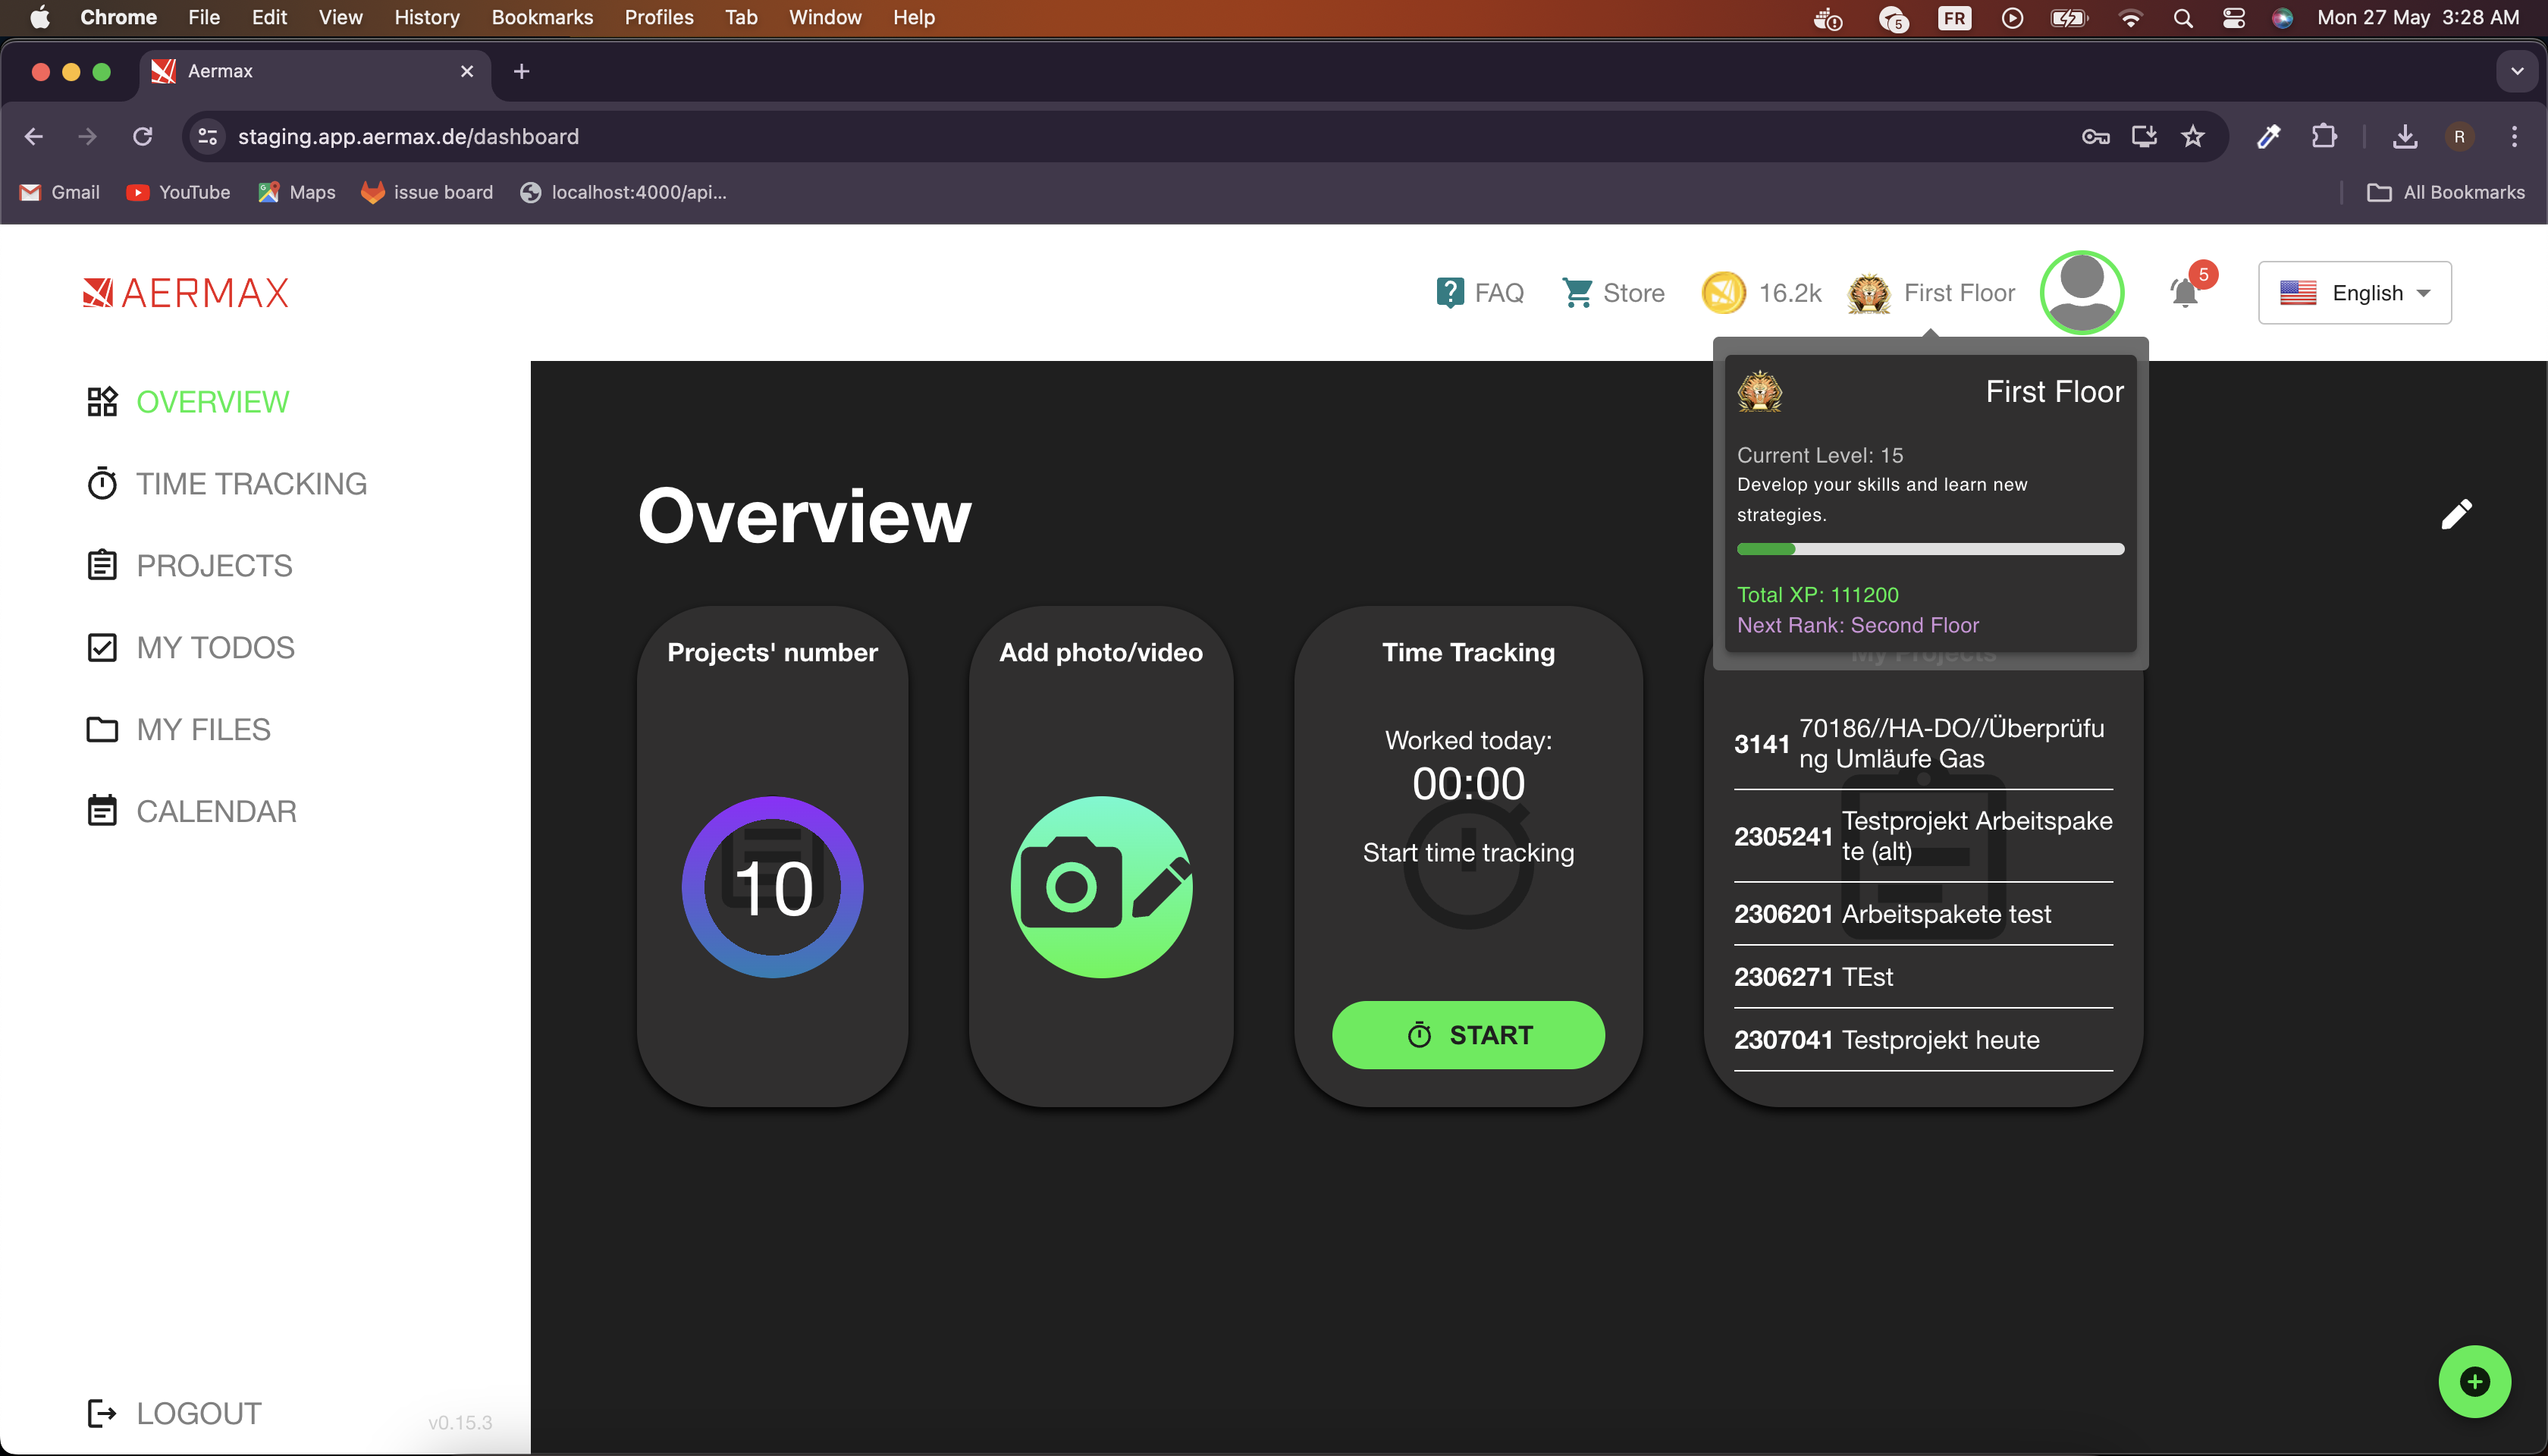
\includegraphics[width=1\textwidth]{src/assets/chapters/subcompanyoverview.png}
  \caption{Aermax Subcompany User Overview}
  \label{fig:sub-login}
\end{figure}

When we login as subcompany users, we notice the same dashboard as the admin has yet with limited informations.
We will focus just on the Reward System Features.


\subsection{Monitoring}
\subsubsection{Introduction}
Improvement in visibility is certainly achieved through the use of dashboards. As a result, we have implemented monitoring solutions for our entire cluster. The elements we keep track are the logs of our microservices. Our initial step involves exposing the Kubernetes dashboard using manifest resources and kubectl.

\subsubsection{Monitoring the logs}

In order to adequately oversee the logs of our diverse microservices and other applications operating on the cluster, we should:

\begin{itemize}
  \item Gather the logs from the various Pods in the cluster
  \item Transform and analyze the logs into a standardized format, typically JSON
  \item Transmit the logs to a search engine for effortless retrieval
  \item Optionally produce dashboards for our logs

\end{itemize}

\paragraph{}
The most effective method for this task is to utilize the EFK Stack, which comprises Elasticsearch, Fluentd, and Kibana.

\textbf{Elasticsearch:}

Elasticsearch has many uses, such as being a search engine, an analytics engine, or even a database. It can handle large amounts of logs using minimal resources, which makes it the optimal choice for our cluster.


Kibana, a data visualization dashboard, is specifically designed to work with Elasticsearch and is commonly utilized in conjunction with an Elasticsearch instance.


Utilizing the open-source \textbf{Elastic Stack Kubernetes Helm Charts} allows us to establish our Elasticsearch and Kibana configuration within the cluster.

\begin{figure}[H]
  \centering
  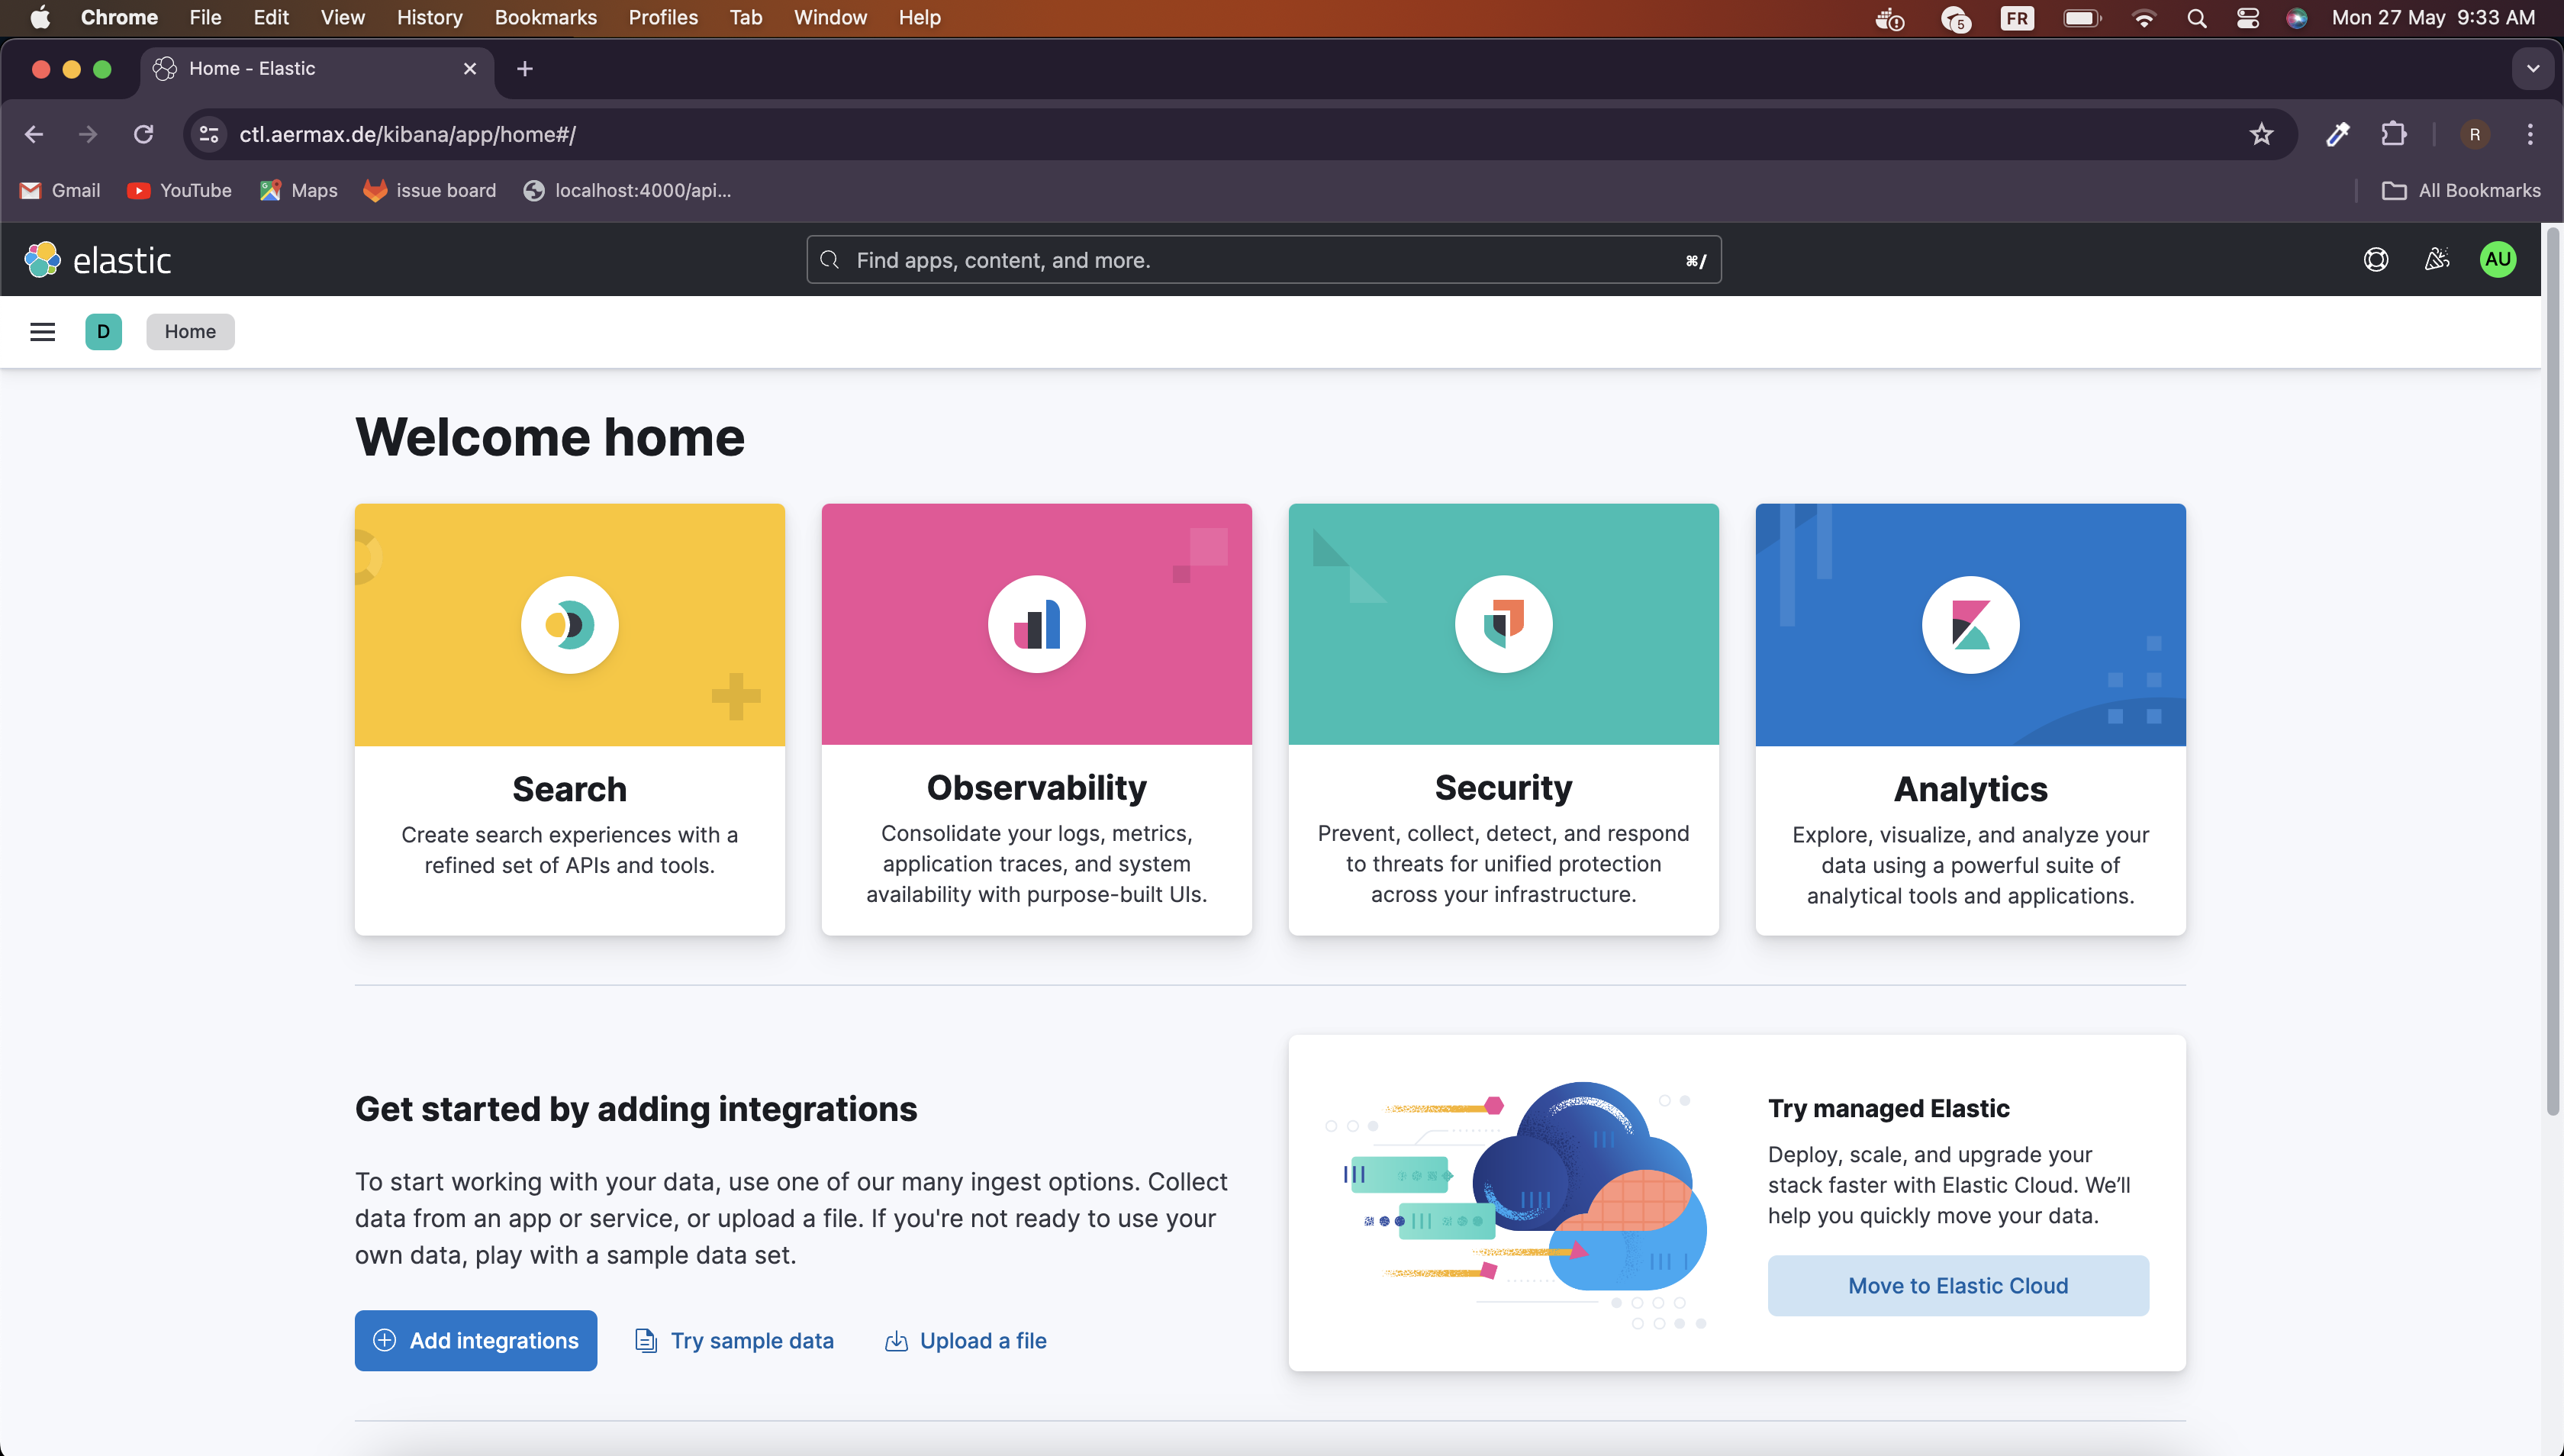
\includegraphics[width=1\textwidth]{src/assets/chapters/elastic.png}
  \caption{Kibana dashboard}
  \label{fig:kibana-dash}
\end{figure}


\textbf{Fluentd:}


Fluentd, however, serves as a data aggregator. Its main function is to operate in the background and ensure that our applications' logs are delivered to any specified service in a consistent manner. We set it up to retrieve logs from our Pods' standard output, convert them to JSON, and then transmit them to Elasticsearch.

After the deployment, we have the option to leverage advanced Elasticsearch features like filtering and sorting our logs directly from the Kibana dashboard.

\begin{figure}[H]
  \centering
  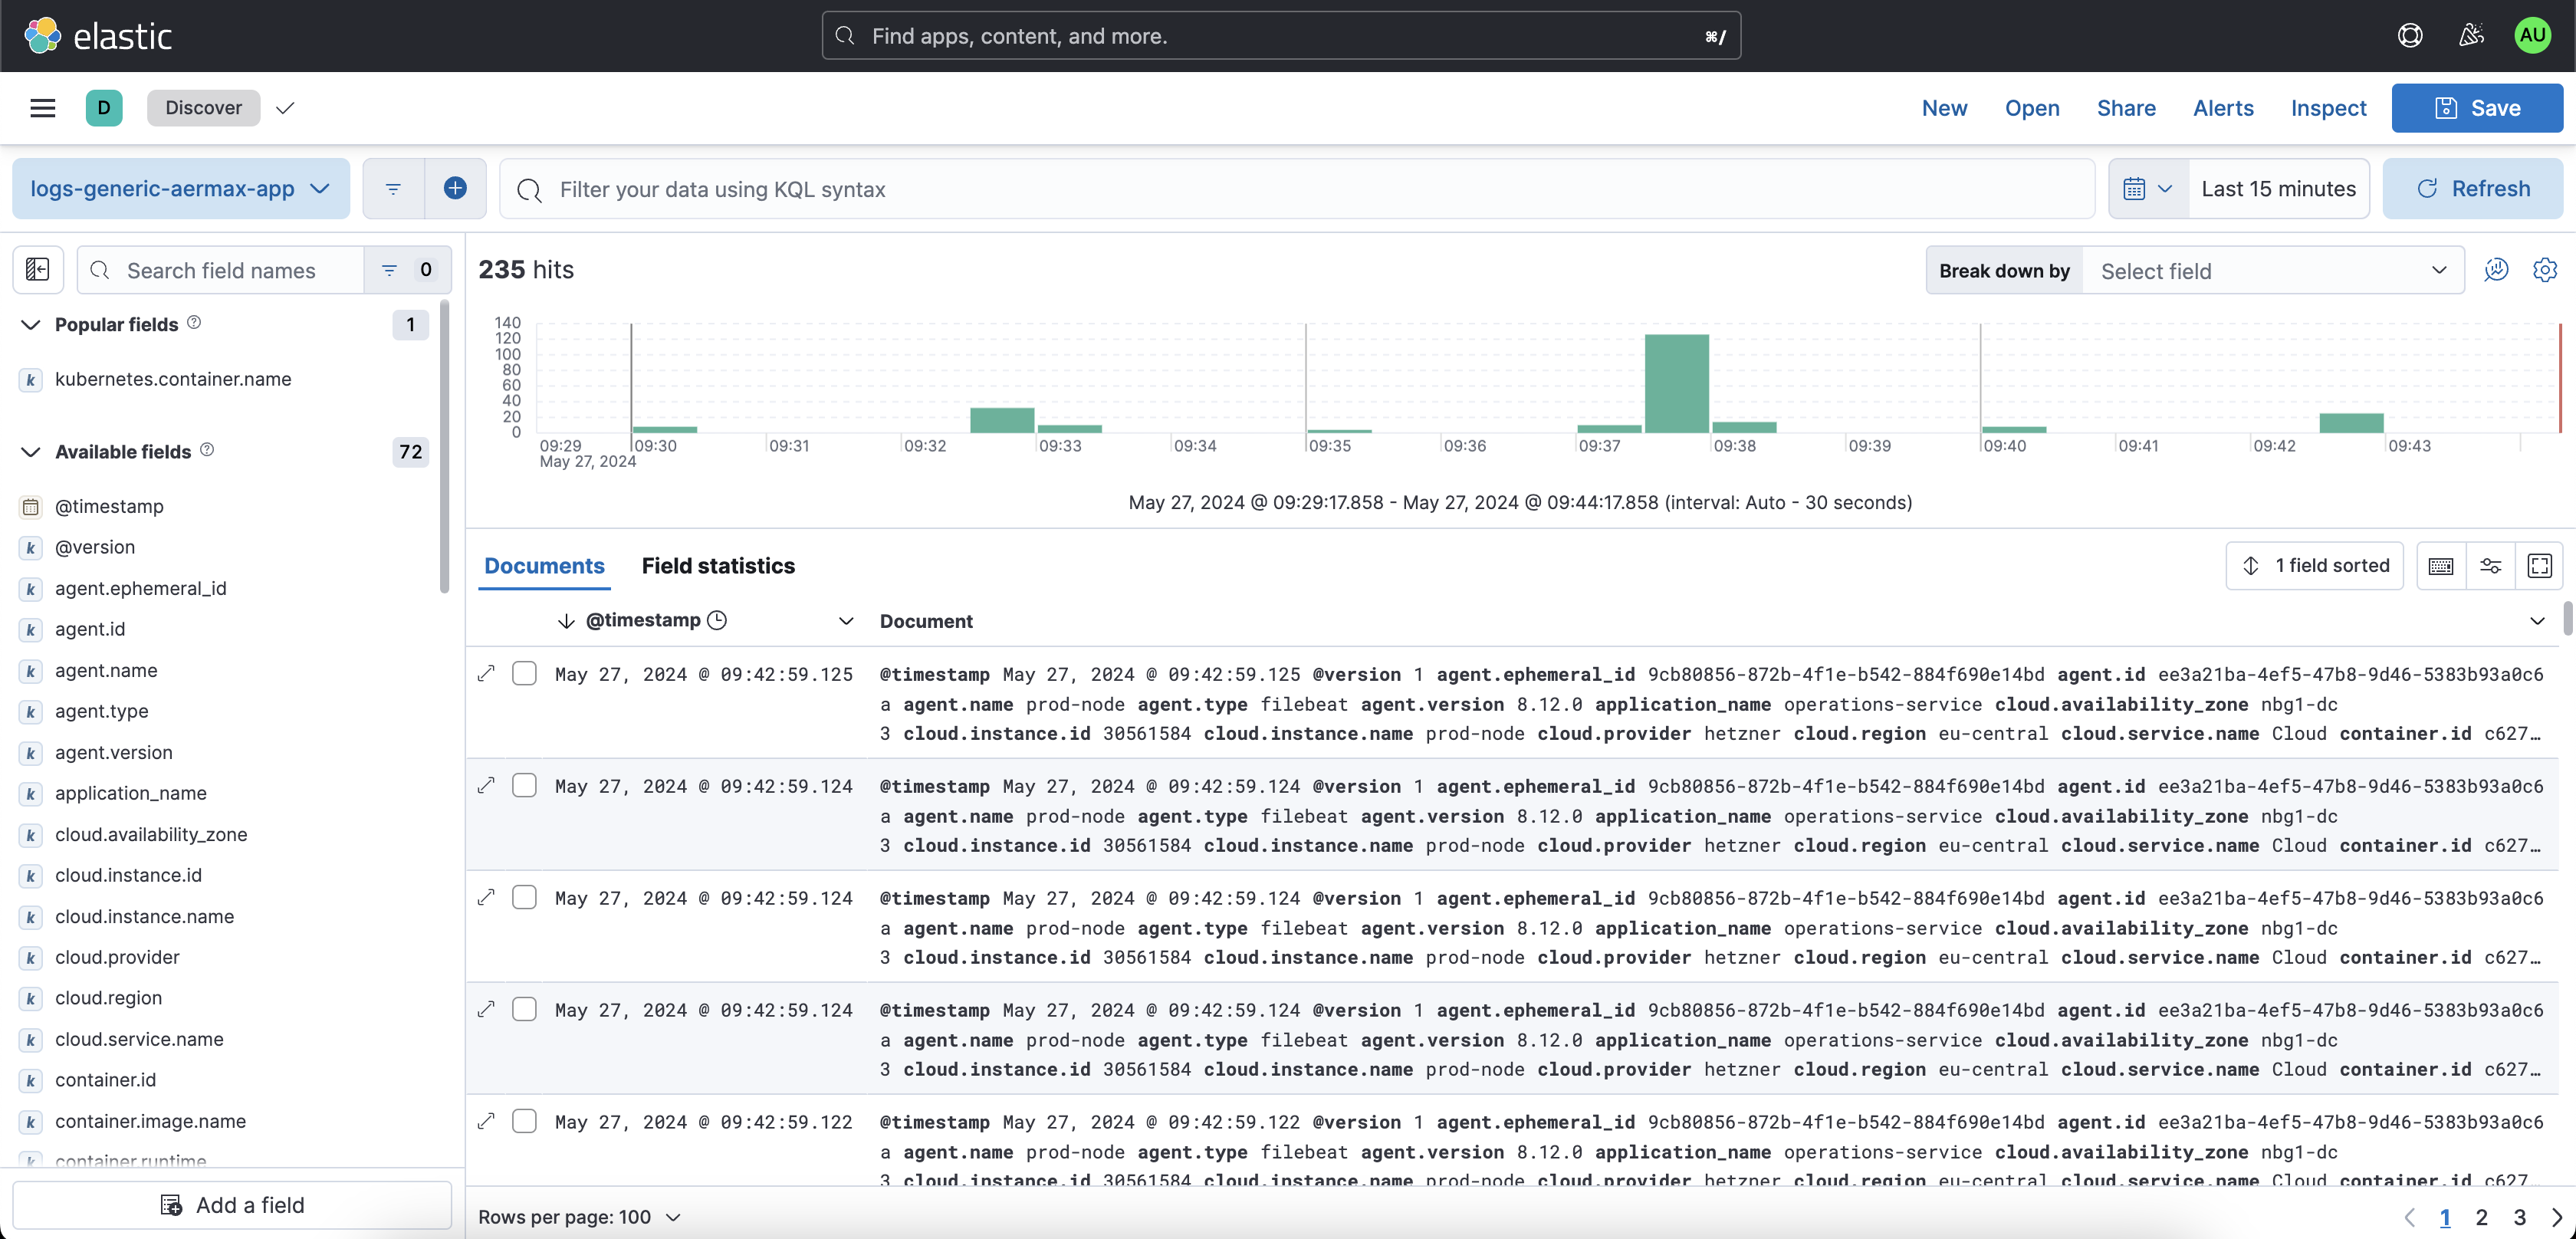
\includegraphics[width=1\textwidth]{src/assets/chapters/kibanalogs1.png}
  \caption{Kibana Dashboard Logs(1)}
  \label{fig:kibana-dash-logs-1}
\end{figure}

\begin{figure}[H]
  \centering
  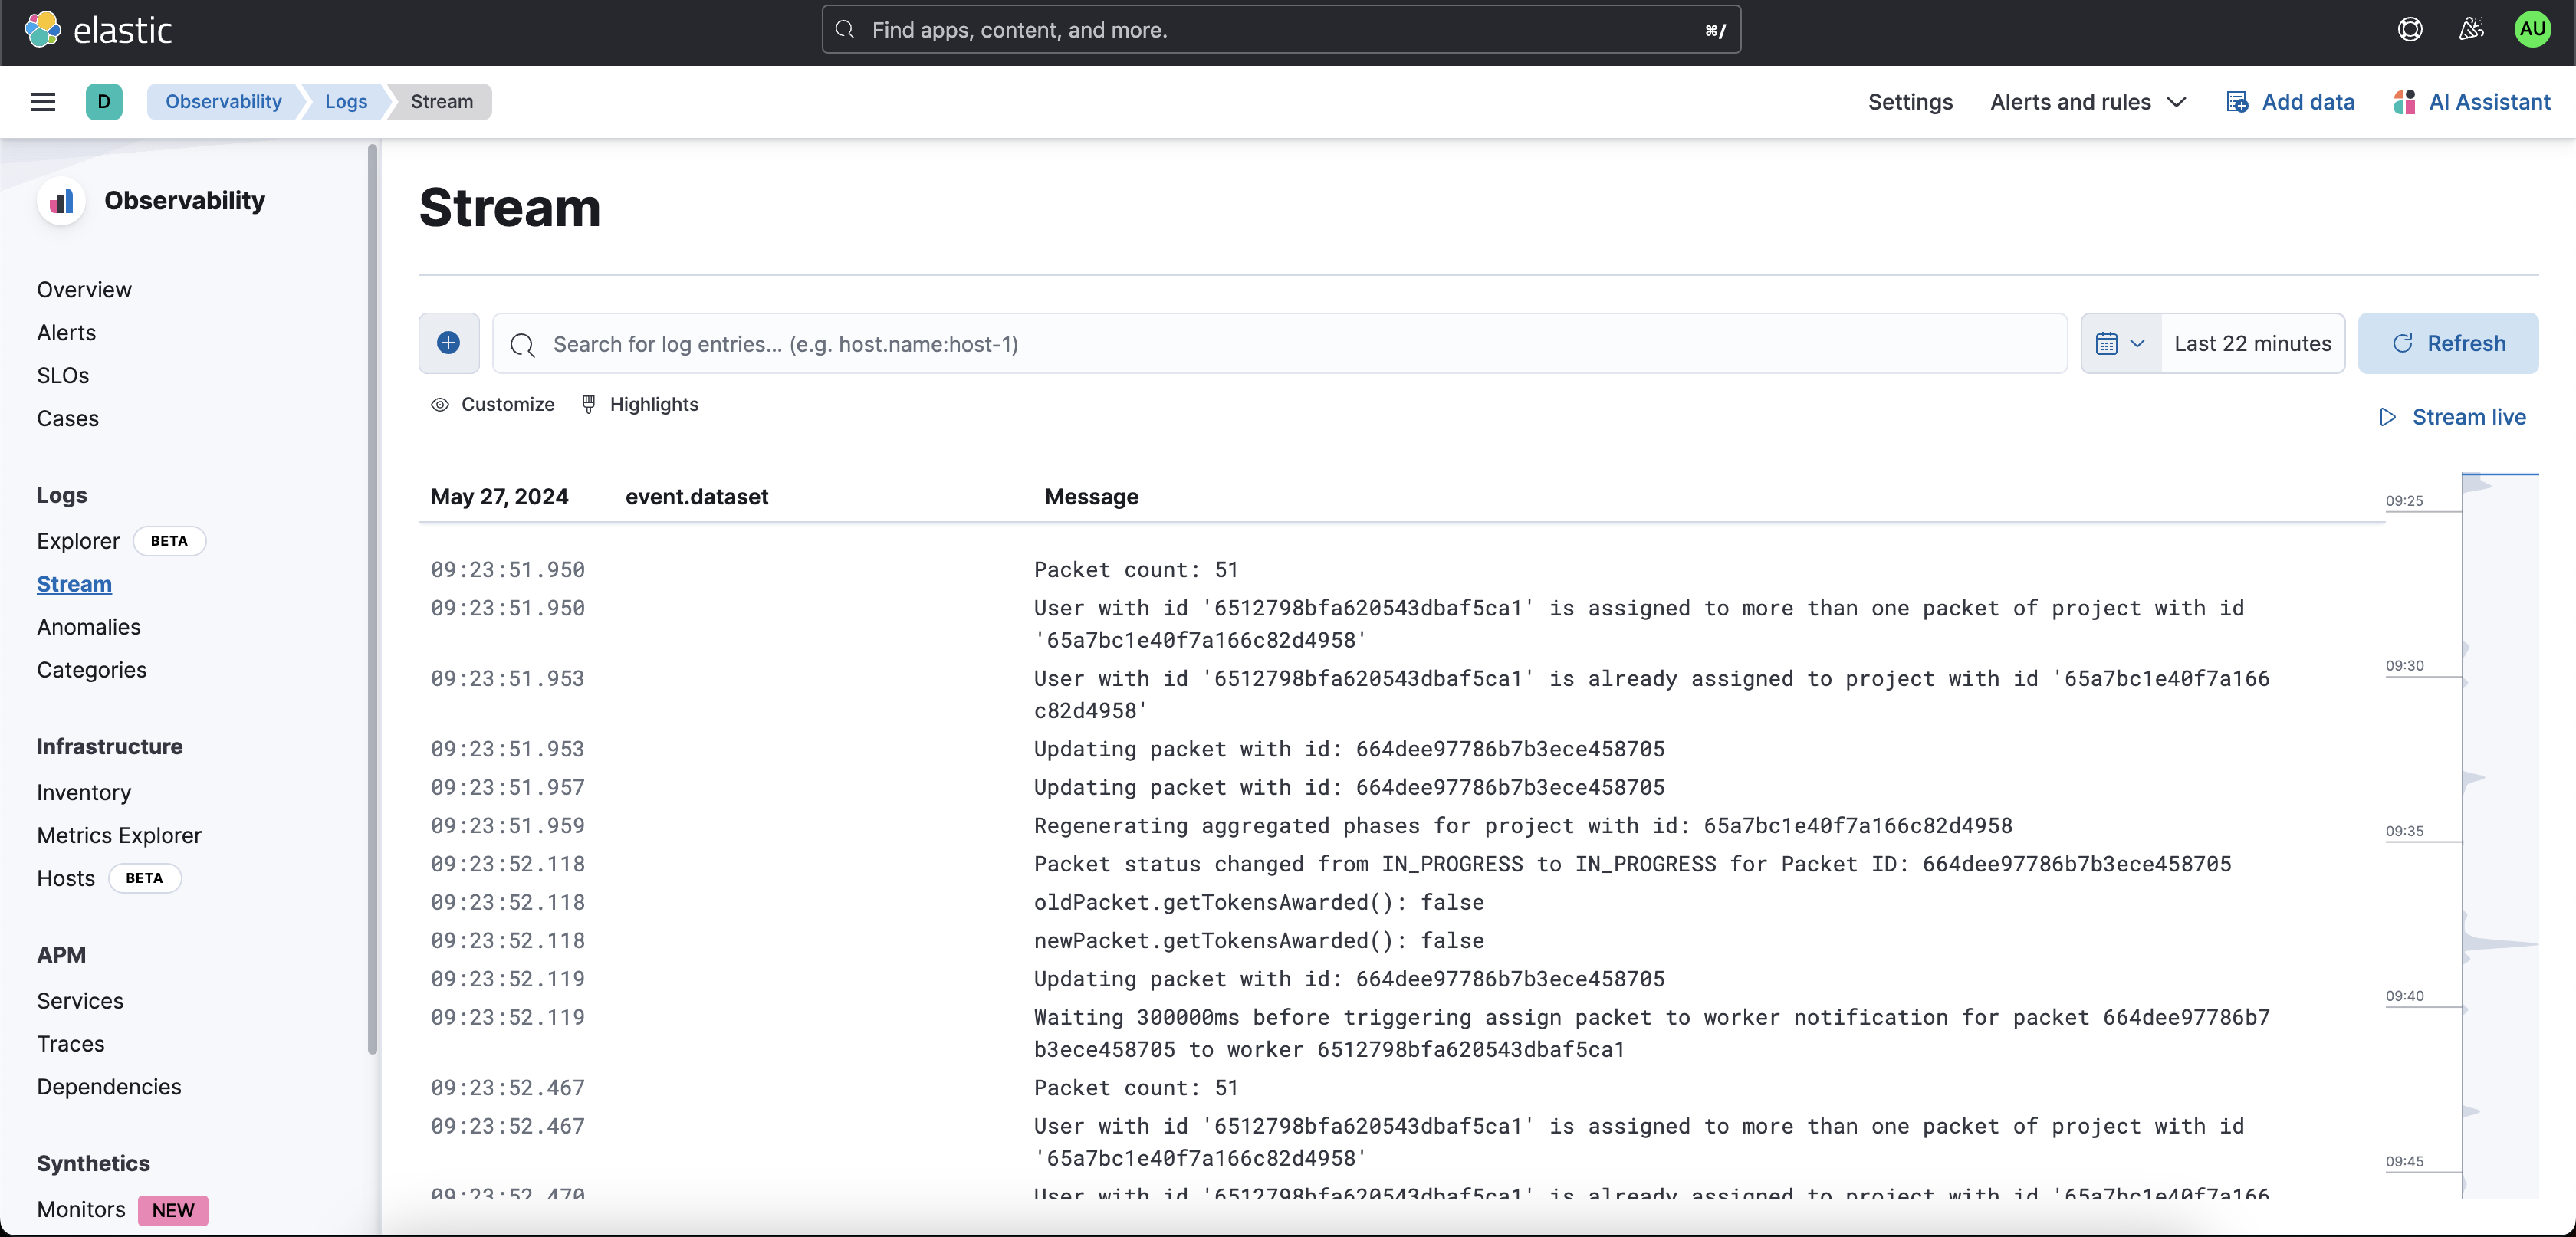
\includegraphics[width=1\textwidth]{src/assets/chapters/kibanalogs2.png}
  \caption{Kibana Dashboard Logs(2)}
  \label{fig:kibana-dash-logs-2}
\end{figure}


\setcounter{secnumdepth}{0}
\section{Conclusion}
For a project to be successful, it is essential to establish a well-structured development environment and an efficient production environment with robust monitoring solutions. We spent a considerable amount of time configuring the infrastructure in a scalable and contemporary manner using different tools and scripts that follow DevOps best practices.